\documentclass[twoside]{book}

% Packages required by doxygen
\usepackage{calc}
\usepackage{doxygen}
\usepackage{graphicx}
\usepackage[utf8]{inputenc}
\usepackage{makeidx}
\usepackage{multicol}
\usepackage{multirow}
\usepackage{textcomp}
\usepackage[table]{xcolor}

% Font selection
\usepackage[T1]{fontenc}
\usepackage{mathptmx}
\usepackage[scaled=.90]{helvet}
\usepackage{courier}
\usepackage{amssymb}
\usepackage{sectsty}
\renewcommand{\familydefault}{\sfdefault}
\allsectionsfont{%
  \fontseries{bc}\selectfont%
  \color{darkgray}%
}
\renewcommand{\DoxyLabelFont}{%
  \fontseries{bc}\selectfont%
  \color{darkgray}%
}

% Page & text layout
\usepackage{geometry}
\geometry{%
  a4paper,%
  top=2.5cm,%
  bottom=2.5cm,%
  left=2.5cm,%
  right=2.5cm%
}
\tolerance=750
\hfuzz=15pt
\hbadness=750
\setlength{\emergencystretch}{15pt}
\setlength{\parindent}{0cm}
\setlength{\parskip}{0.2cm}
\makeatletter
\renewcommand{\paragraph}{%
  \@startsection{paragraph}{4}{0ex}{-1.0ex}{1.0ex}{%
    \normalfont\normalsize\bfseries\SS@parafont%
  }%
}
\renewcommand{\subparagraph}{%
  \@startsection{subparagraph}{5}{0ex}{-1.0ex}{1.0ex}{%
    \normalfont\normalsize\bfseries\SS@subparafont%
  }%
}
\makeatother

% Headers & footers
\usepackage{fancyhdr}
\pagestyle{fancyplain}
\fancyhead[LE]{\fancyplain{}{\bfseries\thepage}}
\fancyhead[CE]{\fancyplain{}{}}
\fancyhead[RE]{\fancyplain{}{\bfseries\leftmark}}
\fancyhead[LO]{\fancyplain{}{\bfseries\rightmark}}
\fancyhead[CO]{\fancyplain{}{}}
\fancyhead[RO]{\fancyplain{}{\bfseries\thepage}}
\fancyfoot[LE]{\fancyplain{}{}}
\fancyfoot[CE]{\fancyplain{}{}}
\fancyfoot[RE]{\fancyplain{}{\bfseries\scriptsize Generated on Wed Dec 18 2013 15\-:48\-:28 for My Project by Doxygen }}
\fancyfoot[LO]{\fancyplain{}{\bfseries\scriptsize Generated on Wed Dec 18 2013 15\-:48\-:28 for My Project by Doxygen }}
\fancyfoot[CO]{\fancyplain{}{}}
\fancyfoot[RO]{\fancyplain{}{}}
\renewcommand{\footrulewidth}{0.4pt}
\renewcommand{\chaptermark}[1]{%
  \markboth{#1}{}%
}
\renewcommand{\sectionmark}[1]{%
  \markright{\thesection\ #1}%
}

% Indices & bibliography
\usepackage{natbib}
\usepackage[titles]{tocloft}
\setcounter{tocdepth}{3}
\setcounter{secnumdepth}{5}
\makeindex

% Hyperlinks (required, but should be loaded last)
\usepackage{ifpdf}
\ifpdf
  \usepackage[pdftex,pagebackref=true]{hyperref}
\else
  \usepackage[ps2pdf,pagebackref=true]{hyperref}
\fi
\hypersetup{%
  colorlinks=true,%
  linkcolor=blue,%
  citecolor=blue,%
  unicode%
}

% Custom commands
\newcommand{\clearemptydoublepage}{%
  \newpage{\pagestyle{empty}\cleardoublepage}%
}


%===== C O N T E N T S =====

\begin{document}

% Titlepage & ToC
\hypersetup{pageanchor=false}
\pagenumbering{roman}
\begin{titlepage}
\vspace*{7cm}
\begin{center}%
{\Large My Project }\\
\vspace*{1cm}
{\large Generated by Doxygen 1.8.5}\\
\vspace*{0.5cm}
{\small Wed Dec 18 2013 15:48:28}\\
\end{center}
\end{titlepage}
\clearemptydoublepage
\tableofcontents
\clearemptydoublepage
\pagenumbering{arabic}
\hypersetup{pageanchor=true}

%--- Begin generated contents ---
\chapter{Hierarchical Index}
\section{Class Hierarchy}
This inheritance list is sorted roughly, but not completely, alphabetically\-:\begin{DoxyCompactList}
\item \contentsline{section}{Level\-:\-:Difficulty}{\pageref{structLevel_1_1Difficulty}}{}
\item \contentsline{section}{Game}{\pageref{classGame}}{}
\item \contentsline{section}{Level}{\pageref{classLevel}}{}
\begin{DoxyCompactList}
\item \contentsline{section}{Newlevel}{\pageref{classNewlevel}}{}
\end{DoxyCompactList}
\item \contentsline{section}{Menu}{\pageref{classMenu}}{}
\item \contentsline{section}{Sprite}{\pageref{classSprite}}{}
\begin{DoxyCompactList}
\item \contentsline{section}{Arrow}{\pageref{classArrow}}{}
\item \contentsline{section}{Player}{\pageref{classPlayer}}{}
\item \contentsline{section}{Ui}{\pageref{classUi}}{}
\item \contentsline{section}{Zombie}{\pageref{classZombie}}{}
\end{DoxyCompactList}
\item \contentsline{section}{Timer}{\pageref{classTimer}}{}
\end{DoxyCompactList}

\chapter{Class Index}
\section{Class List}
Here are the classes, structs, unions and interfaces with brief descriptions\-:\begin{DoxyCompactList}
\item\contentsline{section}{\hyperlink{classArrow}{Arrow} }{\pageref{classArrow}}{}
\item\contentsline{section}{\hyperlink{structLevel_1_1Difficulty}{Level\-::\-Difficulty} }{\pageref{structLevel_1_1Difficulty}}{}
\item\contentsline{section}{\hyperlink{classGame}{Game} }{\pageref{classGame}}{}
\item\contentsline{section}{\hyperlink{classLevel}{Level} }{\pageref{classLevel}}{}
\item\contentsline{section}{\hyperlink{classMenu}{Menu} }{\pageref{classMenu}}{}
\item\contentsline{section}{\hyperlink{classNewlevel}{Newlevel} }{\pageref{classNewlevel}}{}
\item\contentsline{section}{\hyperlink{classPlayer}{Player} }{\pageref{classPlayer}}{}
\item\contentsline{section}{\hyperlink{classSprite}{Sprite} }{\pageref{classSprite}}{}
\item\contentsline{section}{\hyperlink{classTimer}{Timer} }{\pageref{classTimer}}{}
\item\contentsline{section}{\hyperlink{classUi}{Ui} }{\pageref{classUi}}{}
\item\contentsline{section}{\hyperlink{classZombie}{Zombie} }{\pageref{classZombie}}{}
\end{DoxyCompactList}

\chapter{File Index}
\section{File List}
Here is a list of all files with brief descriptions\-:\begin{DoxyCompactList}
\item\contentsline{section}{\hyperlink{arrow_8cc}{arrow.\-cc} }{\pageref{arrow_8cc}}{}
\item\contentsline{section}{\hyperlink{arrow_8h}{arrow.\-h} }{\pageref{arrow_8h}}{}
\item\contentsline{section}{\hyperlink{game_8cc}{game.\-cc} }{\pageref{game_8cc}}{}
\item\contentsline{section}{\hyperlink{game_8h}{game.\-h} }{\pageref{game_8h}}{}
\item\contentsline{section}{\hyperlink{level_8cc}{level.\-cc} }{\pageref{level_8cc}}{}
\item\contentsline{section}{\hyperlink{level_8h}{level.\-h} }{\pageref{level_8h}}{}
\item\contentsline{section}{\hyperlink{main_8cc}{main.\-cc} }{\pageref{main_8cc}}{}
\item\contentsline{section}{\hyperlink{menu_8cc}{menu.\-cc} }{\pageref{menu_8cc}}{}
\item\contentsline{section}{\hyperlink{menu_8h}{menu.\-h} }{\pageref{menu_8h}}{}
\item\contentsline{section}{\hyperlink{newlevel_8cc}{newlevel.\-cc} }{\pageref{newlevel_8cc}}{}
\item\contentsline{section}{\hyperlink{newlevel_8h}{newlevel.\-h} }{\pageref{newlevel_8h}}{}
\item\contentsline{section}{\hyperlink{player_8cc}{player.\-cc} }{\pageref{player_8cc}}{}
\item\contentsline{section}{\hyperlink{player_8h}{player.\-h} }{\pageref{player_8h}}{}
\item\contentsline{section}{\hyperlink{sprite_8cc}{sprite.\-cc} }{\pageref{sprite_8cc}}{}
\item\contentsline{section}{\hyperlink{sprite_8h}{sprite.\-h} }{\pageref{sprite_8h}}{}
\item\contentsline{section}{\hyperlink{timer_8cc}{timer.\-cc} }{\pageref{timer_8cc}}{}
\item\contentsline{section}{\hyperlink{timer_8h}{timer.\-h} }{\pageref{timer_8h}}{}
\item\contentsline{section}{\hyperlink{UI_8cc}{U\-I.\-cc} }{\pageref{UI_8cc}}{}
\item\contentsline{section}{\hyperlink{UI_8cpp}{U\-I.\-cpp} }{\pageref{UI_8cpp}}{}
\item\contentsline{section}{\hyperlink{UI_8h}{U\-I.\-h} }{\pageref{UI_8h}}{}
\item\contentsline{section}{\hyperlink{zombie_8cc}{zombie.\-cc} }{\pageref{zombie_8cc}}{}
\item\contentsline{section}{\hyperlink{zombie_8h}{zombie.\-h} }{\pageref{zombie_8h}}{}
\end{DoxyCompactList}

\chapter{Class Documentation}
\hypertarget{classArrow}{\section{Arrow Class Reference}
\label{classArrow}\index{Arrow@{Arrow}}
}


{\ttfamily \#include $<$arrow.\-h$>$}



Inheritance diagram for Arrow\-:\nopagebreak
\begin{figure}[H]
\begin{center}
\leavevmode
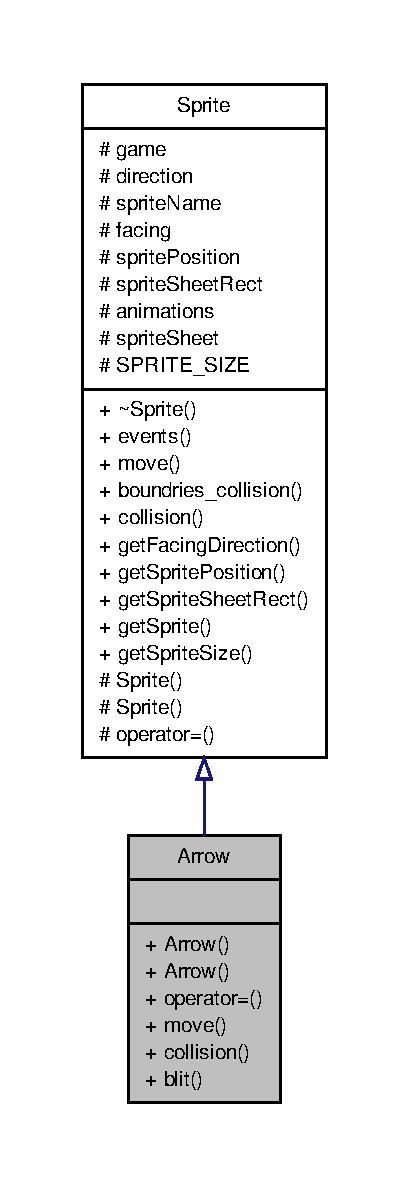
\includegraphics[height=550pt]{classArrow__inherit__graph}
\end{center}
\end{figure}


Collaboration diagram for Arrow\-:
\nopagebreak
\begin{figure}[H]
\begin{center}
\leavevmode
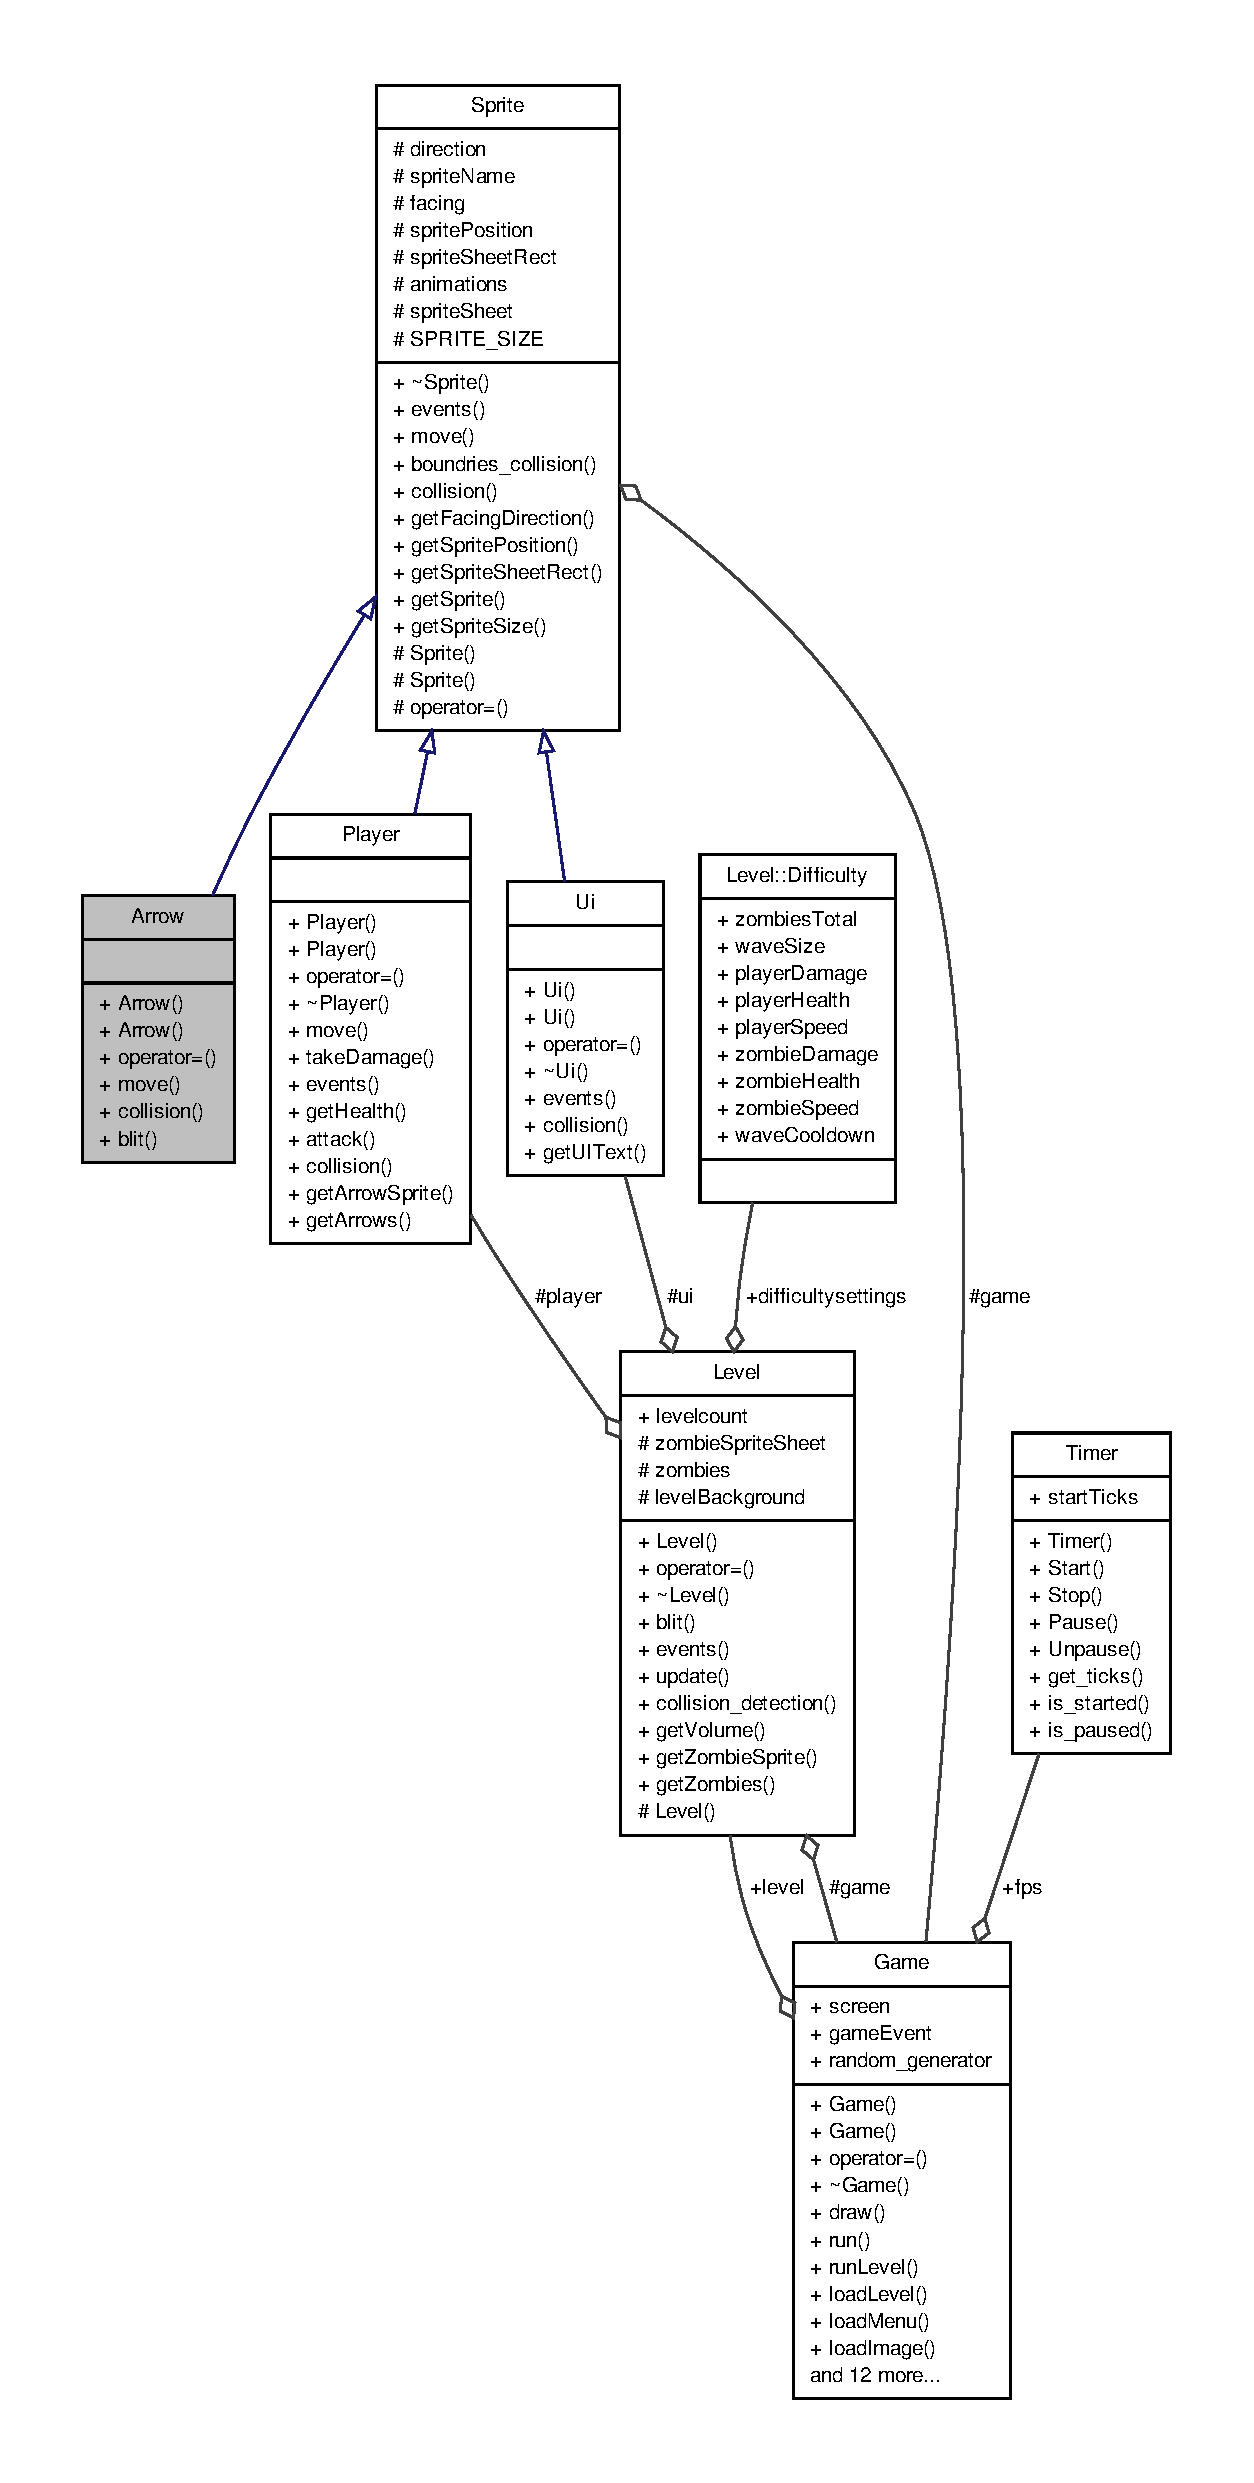
\includegraphics[height=550pt]{classArrow__coll__graph}
\end{center}
\end{figure}
\subsection*{Public Member Functions}
\begin{DoxyCompactItemize}
\item 
\hyperlink{classArrow_ae134c1249c785d8921886c355bac8972}{Arrow} (\hyperlink{classGame}{Game} $\ast$game\-Pointer, \hyperlink{classPlayer}{Player} $\ast$player, \hyperlink{classLevel}{Level} $\ast$level, std\-::string facing\-\_\-direction, S\-D\-L\-\_\-\-Rect player\-Position)
\item 
\hyperlink{classArrow_a3eacdef1aee0243a65d738f9723916f8}{Arrow} (const \hyperlink{classArrow}{Arrow} \&)=delete
\item 
\hyperlink{classArrow}{Arrow} \& \hyperlink{classArrow_a764fe70858bda2a51d61316bac67397d}{operator=} (const \hyperlink{classArrow}{Arrow} \&)=delete
\item 
void \hyperlink{classArrow_aab8bcf5d8e523c6d992c96af645dd30a}{move} ()
\item 
bool \hyperlink{classArrow_aab2752bc7867eb7595a959189e0eb667}{collision} ()
\item 
void \hyperlink{classArrow_afdc36c090185454d3630a4248e3f9e62}{blit} ()
\end{DoxyCompactItemize}
\subsection*{Additional Inherited Members}


\subsection{Constructor \& Destructor Documentation}
\hypertarget{classArrow_ae134c1249c785d8921886c355bac8972}{\index{Arrow@{Arrow}!Arrow@{Arrow}}
\index{Arrow@{Arrow}!Arrow@{Arrow}}
\subsubsection[{Arrow}]{\setlength{\rightskip}{0pt plus 5cm}Arrow\-::\-Arrow (
\begin{DoxyParamCaption}
\item[{{\bf Game} $\ast$}]{game\-Pointer, }
\item[{{\bf Player} $\ast$}]{player, }
\item[{{\bf Level} $\ast$}]{level, }
\item[{std\-::string}]{facing\-\_\-direction, }
\item[{S\-D\-L\-\_\-\-Rect}]{player\-Position}
\end{DoxyParamCaption}
)}}\label{classArrow_ae134c1249c785d8921886c355bac8972}
arrow constructor contains settings for the arrows speed, size, sprite sheet positions and which direction it is facing when fired.\hypertarget{classArrow_a3eacdef1aee0243a65d738f9723916f8}{\index{Arrow@{Arrow}!Arrow@{Arrow}}
\index{Arrow@{Arrow}!Arrow@{Arrow}}
\subsubsection[{Arrow}]{\setlength{\rightskip}{0pt plus 5cm}Arrow\-::\-Arrow (
\begin{DoxyParamCaption}
\item[{const {\bf Arrow} \&}]{}
\end{DoxyParamCaption}
)\hspace{0.3cm}{\ttfamily [delete]}}}\label{classArrow_a3eacdef1aee0243a65d738f9723916f8}


\subsection{Member Function Documentation}
\hypertarget{classArrow_afdc36c090185454d3630a4248e3f9e62}{\index{Arrow@{Arrow}!blit@{blit}}
\index{blit@{blit}!Arrow@{Arrow}}
\subsubsection[{blit}]{\setlength{\rightskip}{0pt plus 5cm}void Arrow\-::blit (
\begin{DoxyParamCaption}
{}
\end{DoxyParamCaption}
)}}\label{classArrow_afdc36c090185454d3630a4248e3f9e62}
\hypertarget{classArrow_aab2752bc7867eb7595a959189e0eb667}{\index{Arrow@{Arrow}!collision@{collision}}
\index{collision@{collision}!Arrow@{Arrow}}
\subsubsection[{collision}]{\setlength{\rightskip}{0pt plus 5cm}bool Arrow\-::collision (
\begin{DoxyParamCaption}
{}
\end{DoxyParamCaption}
)\hspace{0.3cm}{\ttfamily [virtual]}}}\label{classArrow_aab2752bc7867eb7595a959189e0eb667}
iterate through all zombies on the level and check if the arrow collided with any of them, if so then do dammage on these foes!

Implements \hyperlink{classSprite_ae0c21af6a4fc7fb8e9daf72675a1ec50}{Sprite}.

\hypertarget{classArrow_aab8bcf5d8e523c6d992c96af645dd30a}{\index{Arrow@{Arrow}!move@{move}}
\index{move@{move}!Arrow@{Arrow}}
\subsubsection[{move}]{\setlength{\rightskip}{0pt plus 5cm}void Arrow\-::move (
\begin{DoxyParamCaption}
{}
\end{DoxyParamCaption}
)\hspace{0.3cm}{\ttfamily [virtual]}}}\label{classArrow_aab8bcf5d8e523c6d992c96af645dd30a}
move uses the arrows direction to calculate in which direction to move.

Reimplemented from \hyperlink{classSprite_afcf196c3d93fd743fdcc6f84d128ece6}{Sprite}.

\hypertarget{classArrow_a764fe70858bda2a51d61316bac67397d}{\index{Arrow@{Arrow}!operator=@{operator=}}
\index{operator=@{operator=}!Arrow@{Arrow}}
\subsubsection[{operator=}]{\setlength{\rightskip}{0pt plus 5cm}{\bf Arrow}\& Arrow\-::operator= (
\begin{DoxyParamCaption}
\item[{const {\bf Arrow} \&}]{}
\end{DoxyParamCaption}
)\hspace{0.3cm}{\ttfamily [delete]}}}\label{classArrow_a764fe70858bda2a51d61316bac67397d}


The documentation for this class was generated from the following files\-:\begin{DoxyCompactItemize}
\item 
\hyperlink{arrow_8h}{arrow.\-h}\item 
\hyperlink{arrow_8cc}{arrow.\-cc}\end{DoxyCompactItemize}

\hypertarget{structLevel_1_1Difficulty}{\section{Level\-:\-:Difficulty Struct Reference}
\label{structLevel_1_1Difficulty}\index{Level\-::\-Difficulty@{Level\-::\-Difficulty}}
}


{\ttfamily \#include $<$level.\-h$>$}



Collaboration diagram for Level\-:\-:Difficulty\-:\nopagebreak
\begin{figure}[H]
\begin{center}
\leavevmode
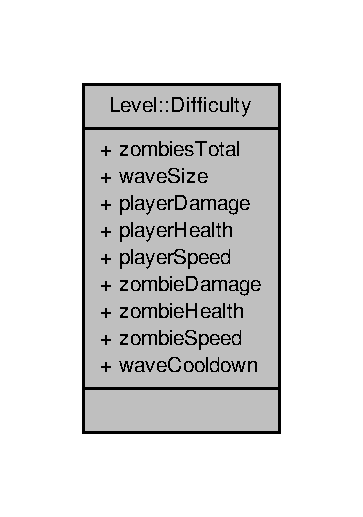
\includegraphics[width=174pt]{structLevel_1_1Difficulty__coll__graph}
\end{center}
\end{figure}
\subsection*{Public Attributes}
\begin{DoxyCompactItemize}
\item 
unsigned int \hyperlink{structLevel_1_1Difficulty_adde47502037079e2c1552140e1aecbe0}{zombies\-Total}
\item 
unsigned int \hyperlink{structLevel_1_1Difficulty_a8c66cad375ccda67a95f9430b3354488}{wave\-Size}
\item 
unsigned int \hyperlink{structLevel_1_1Difficulty_a79ae994f2fa39128956f639f858e0b02}{player\-Damage}
\item 
int \hyperlink{structLevel_1_1Difficulty_a888e1da805bb7ecfc97164e885ee6265}{player\-Health}
\item 
unsigned int \hyperlink{structLevel_1_1Difficulty_ae64bf4253a073ec5b496634112de2137}{player\-Speed}
\item 
unsigned int \hyperlink{structLevel_1_1Difficulty_a59adf3184823a740957e78f62d39c6df}{zombie\-Damage}
\item 
unsigned int \hyperlink{structLevel_1_1Difficulty_a3c4e883253dcd88fa5f221b2684d22ba}{zombie\-Health}
\item 
unsigned int \hyperlink{structLevel_1_1Difficulty_ad9dfcb0694df92389e64e5a9a2e7316e}{zombie\-Speed}
\item 
Uint32 \hyperlink{structLevel_1_1Difficulty_a13ffa97715443be3d015def5752325cb}{wave\-Cooldown}
\end{DoxyCompactItemize}


\subsection{Member Data Documentation}
\hypertarget{structLevel_1_1Difficulty_a79ae994f2fa39128956f639f858e0b02}{\index{Level\-::\-Difficulty@{Level\-::\-Difficulty}!player\-Damage@{player\-Damage}}
\index{player\-Damage@{player\-Damage}!Level::Difficulty@{Level\-::\-Difficulty}}
\subsubsection[{player\-Damage}]{\setlength{\rightskip}{0pt plus 5cm}unsigned int Level\-::\-Difficulty\-::player\-Damage}}\label{structLevel_1_1Difficulty_a79ae994f2fa39128956f639f858e0b02}
\hypertarget{structLevel_1_1Difficulty_a888e1da805bb7ecfc97164e885ee6265}{\index{Level\-::\-Difficulty@{Level\-::\-Difficulty}!player\-Health@{player\-Health}}
\index{player\-Health@{player\-Health}!Level::Difficulty@{Level\-::\-Difficulty}}
\subsubsection[{player\-Health}]{\setlength{\rightskip}{0pt plus 5cm}int Level\-::\-Difficulty\-::player\-Health}}\label{structLevel_1_1Difficulty_a888e1da805bb7ecfc97164e885ee6265}
\hypertarget{structLevel_1_1Difficulty_ae64bf4253a073ec5b496634112de2137}{\index{Level\-::\-Difficulty@{Level\-::\-Difficulty}!player\-Speed@{player\-Speed}}
\index{player\-Speed@{player\-Speed}!Level::Difficulty@{Level\-::\-Difficulty}}
\subsubsection[{player\-Speed}]{\setlength{\rightskip}{0pt plus 5cm}unsigned int Level\-::\-Difficulty\-::player\-Speed}}\label{structLevel_1_1Difficulty_ae64bf4253a073ec5b496634112de2137}
\hypertarget{structLevel_1_1Difficulty_a13ffa97715443be3d015def5752325cb}{\index{Level\-::\-Difficulty@{Level\-::\-Difficulty}!wave\-Cooldown@{wave\-Cooldown}}
\index{wave\-Cooldown@{wave\-Cooldown}!Level::Difficulty@{Level\-::\-Difficulty}}
\subsubsection[{wave\-Cooldown}]{\setlength{\rightskip}{0pt plus 5cm}Uint32 Level\-::\-Difficulty\-::wave\-Cooldown}}\label{structLevel_1_1Difficulty_a13ffa97715443be3d015def5752325cb}
\hypertarget{structLevel_1_1Difficulty_a8c66cad375ccda67a95f9430b3354488}{\index{Level\-::\-Difficulty@{Level\-::\-Difficulty}!wave\-Size@{wave\-Size}}
\index{wave\-Size@{wave\-Size}!Level::Difficulty@{Level\-::\-Difficulty}}
\subsubsection[{wave\-Size}]{\setlength{\rightskip}{0pt plus 5cm}unsigned int Level\-::\-Difficulty\-::wave\-Size}}\label{structLevel_1_1Difficulty_a8c66cad375ccda67a95f9430b3354488}
\hypertarget{structLevel_1_1Difficulty_a59adf3184823a740957e78f62d39c6df}{\index{Level\-::\-Difficulty@{Level\-::\-Difficulty}!zombie\-Damage@{zombie\-Damage}}
\index{zombie\-Damage@{zombie\-Damage}!Level::Difficulty@{Level\-::\-Difficulty}}
\subsubsection[{zombie\-Damage}]{\setlength{\rightskip}{0pt plus 5cm}unsigned int Level\-::\-Difficulty\-::zombie\-Damage}}\label{structLevel_1_1Difficulty_a59adf3184823a740957e78f62d39c6df}
\hypertarget{structLevel_1_1Difficulty_a3c4e883253dcd88fa5f221b2684d22ba}{\index{Level\-::\-Difficulty@{Level\-::\-Difficulty}!zombie\-Health@{zombie\-Health}}
\index{zombie\-Health@{zombie\-Health}!Level::Difficulty@{Level\-::\-Difficulty}}
\subsubsection[{zombie\-Health}]{\setlength{\rightskip}{0pt plus 5cm}unsigned int Level\-::\-Difficulty\-::zombie\-Health}}\label{structLevel_1_1Difficulty_a3c4e883253dcd88fa5f221b2684d22ba}
\hypertarget{structLevel_1_1Difficulty_ad9dfcb0694df92389e64e5a9a2e7316e}{\index{Level\-::\-Difficulty@{Level\-::\-Difficulty}!zombie\-Speed@{zombie\-Speed}}
\index{zombie\-Speed@{zombie\-Speed}!Level::Difficulty@{Level\-::\-Difficulty}}
\subsubsection[{zombie\-Speed}]{\setlength{\rightskip}{0pt plus 5cm}unsigned int Level\-::\-Difficulty\-::zombie\-Speed}}\label{structLevel_1_1Difficulty_ad9dfcb0694df92389e64e5a9a2e7316e}
\hypertarget{structLevel_1_1Difficulty_adde47502037079e2c1552140e1aecbe0}{\index{Level\-::\-Difficulty@{Level\-::\-Difficulty}!zombies\-Total@{zombies\-Total}}
\index{zombies\-Total@{zombies\-Total}!Level::Difficulty@{Level\-::\-Difficulty}}
\subsubsection[{zombies\-Total}]{\setlength{\rightskip}{0pt plus 5cm}unsigned int Level\-::\-Difficulty\-::zombies\-Total}}\label{structLevel_1_1Difficulty_adde47502037079e2c1552140e1aecbe0}


The documentation for this struct was generated from the following file\-:\begin{DoxyCompactItemize}
\item 
\hyperlink{level_8h}{level.\-h}\end{DoxyCompactItemize}

\hypertarget{classGame}{\section{Game Class Reference}
\label{classGame}\index{Game@{Game}}
}


{\ttfamily \#include $<$game.\-h$>$}



Collaboration diagram for Game\-:
\nopagebreak
\begin{figure}[H]
\begin{center}
\leavevmode
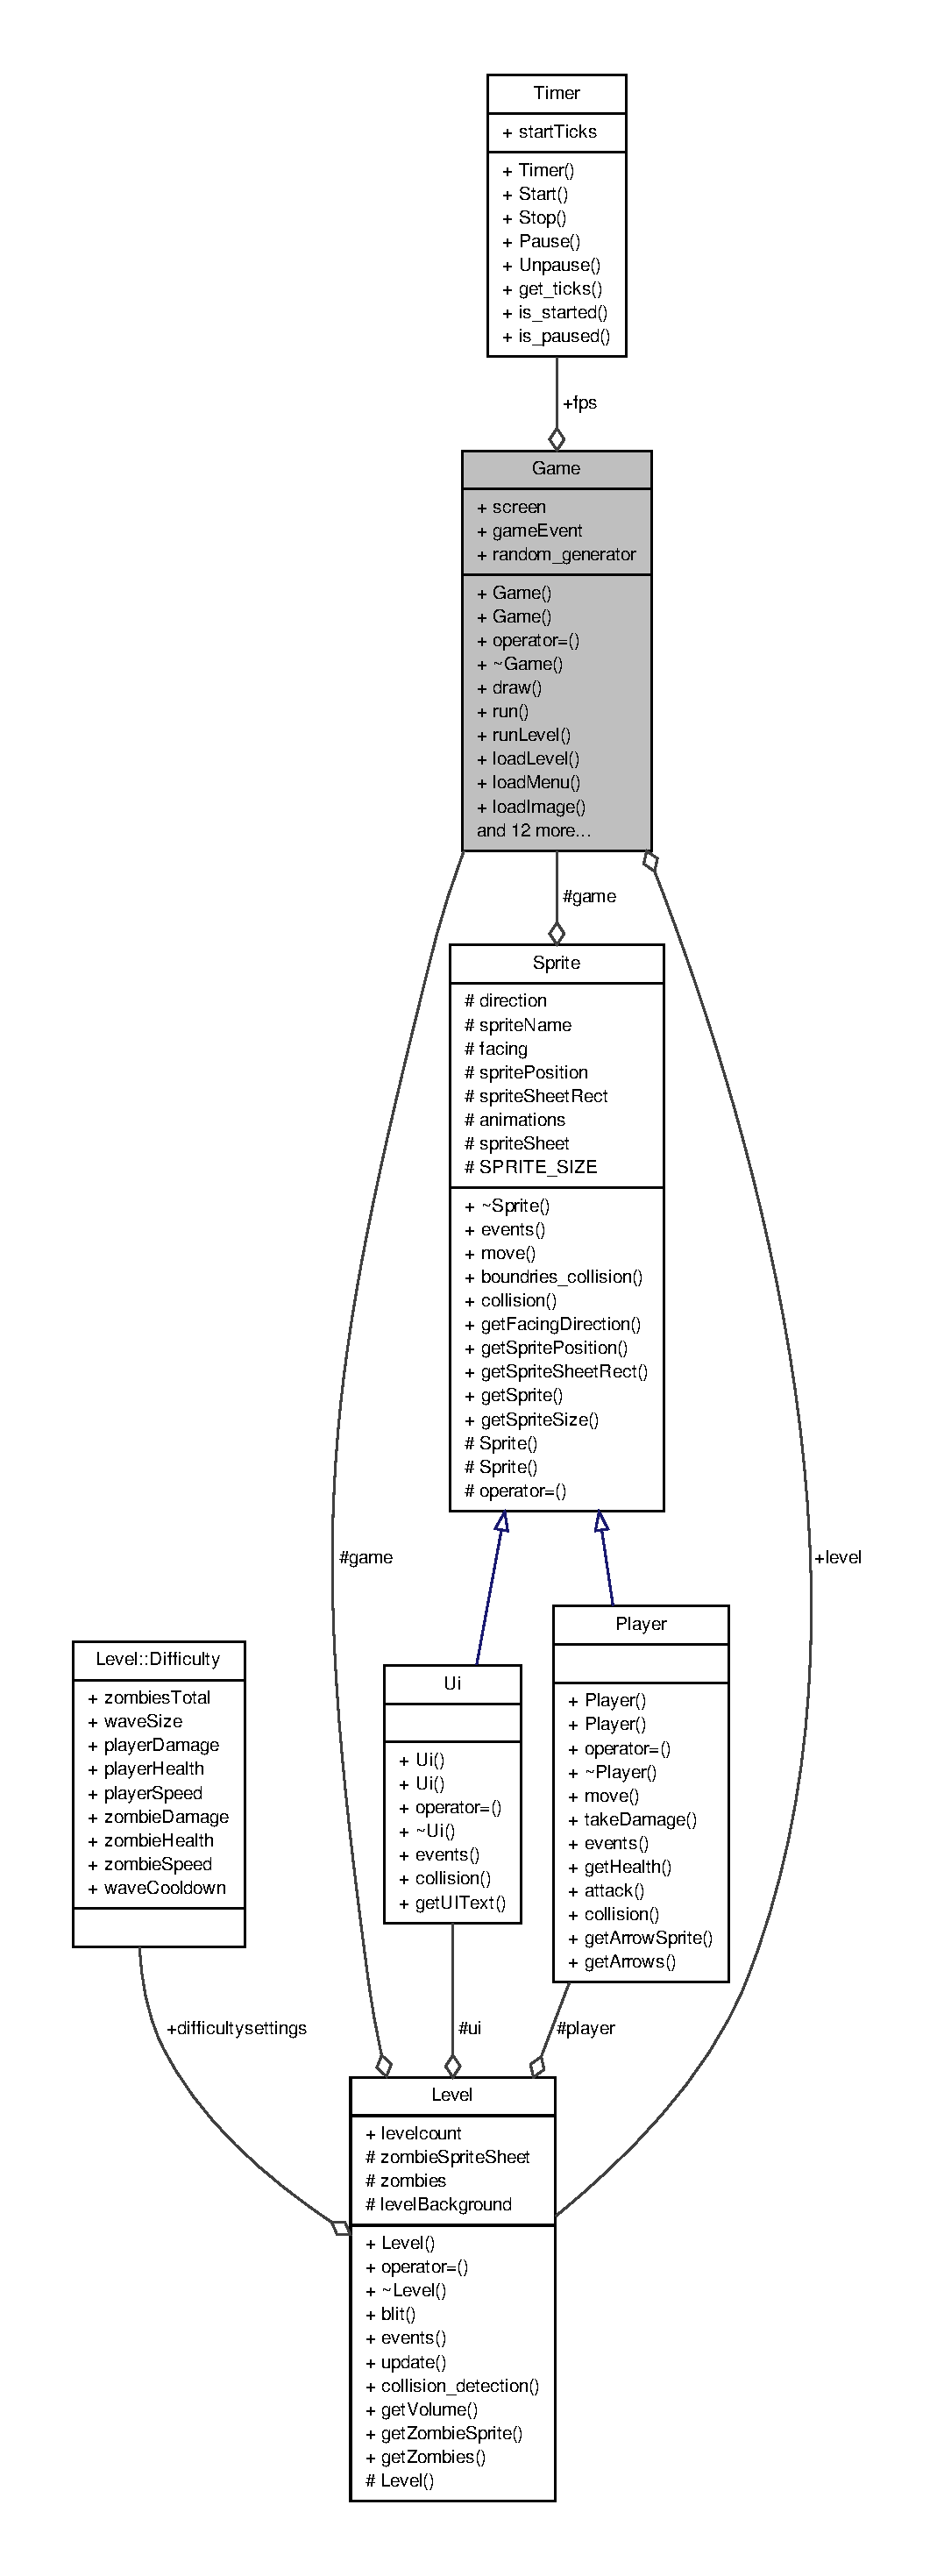
\includegraphics[height=550pt]{classGame__coll__graph}
\end{center}
\end{figure}
\subsection*{Public Types}
\begin{DoxyCompactItemize}
\item 
enum \hyperlink{classGame_a0edcb9debef447b9d0877c8b1d139f24}{States} \{ \\*
\hyperlink{classGame_a0edcb9debef447b9d0877c8b1d139f24a66e2ac0cdacbf1a02a26825feff2ff57}{E\-X\-I\-T}, 
\hyperlink{classGame_a0edcb9debef447b9d0877c8b1d139f24a27b5e3ff6ff653679f76c97fa644b5b4}{M\-E\-N\-U}, 
\hyperlink{classGame_a0edcb9debef447b9d0877c8b1d139f24acf1196c4592cd5e711afe67fa7729699}{P\-L\-A\-Y}, 
\hyperlink{classGame_a0edcb9debef447b9d0877c8b1d139f24a36dbe004786a70a1325e4e345bb02864}{C\-O\-M\-P\-L\-E\-T\-E\-L\-E\-V\-E\-L}, 
\\*
\hyperlink{classGame_a0edcb9debef447b9d0877c8b1d139f24a08d9474d3579084de97a5496d559d1ec}{G\-A\-M\-E\-O\-V\-E\-R}
 \}
\end{DoxyCompactItemize}
\subsection*{Public Member Functions}
\begin{DoxyCompactItemize}
\item 
\hyperlink{classGame_ad59df6562a58a614fda24622d3715b65}{Game} ()
\item 
\hyperlink{classGame_abb28875d74d25fa9e0dcdbe37c6ad89c}{Game} (const \hyperlink{classGame}{Game} \&)=delete
\item 
\hyperlink{classGame}{Game} \& \hyperlink{classGame_a4d0c0503733cc50b0b5cb8d7ef1237ec}{operator=} (const \hyperlink{classGame}{Game} \&)=delete
\item 
\hyperlink{classGame_ae3d112ca6e0e55150d2fdbc704474530}{$\sim$\-Game} ()
\item 
void \hyperlink{classGame_a6d54497ce3a66f6dd45eacfdccc8d0bd}{draw} ()
\item 
void \hyperlink{classGame_a1ab78f5ed0d5ea879157357cf2fb2afa}{run} ()
\item 
void \hyperlink{classGame_a8d5df01e8f891aa5bb01153a66692dd6}{run\-Level} ()
\item 
void \hyperlink{classGame_a9713f011d2d0d3ef4a37aa07d7951947}{load\-Level} ()
\item 
void \hyperlink{classGame_a69c0505b09d39a511eb9c7d44a8cd46e}{load\-Menu} ()
\item 
S\-D\-L\-\_\-\-Surface $\ast$ \hyperlink{classGame_a007a16399b4c563e1a41e1060a7e2db7}{load\-Image} (std\-::string filename)
\item 
void \hyperlink{classGame_a95c19db69b73a56245e41ce9fd639b31}{apply\-Image} (int x, int y, S\-D\-L\-\_\-\-Surface $\ast$source, S\-D\-L\-\_\-\-Surface $\ast$destination, S\-D\-L\-\_\-\-Rect $\ast$sprite\-Clip=N\-U\-L\-L)
\item 
void \hyperlink{classGame_abac16174982079a0c46f0626ada16d54}{play\-Music} (Mix\-\_\-\-Music $\ast$song) const 
\item 
void \hyperlink{classGame_abe33184093d0ae79d40e5ac3521febbb}{play\-Chunk} (Mix\-\_\-\-Chunk $\ast$effect) const 
\item 
Mix\-\_\-\-Music $\ast$ \hyperlink{classGame_a3b0626d1e61c88b1630cd7fd1f9371a9}{load\-Music} (std\-::string filename)
\item 
Mix\-\_\-\-Chunk $\ast$ \hyperlink{classGame_ac5ca4ad10b022c71b07622898c0e17b8}{load\-Chunk} (std\-::string filename)
\item 
void \hyperlink{classGame_aed11a603c8dd060fc5de09e74669a0df}{set\-Game\-State} (int new\-Game\-State)
\item 
int \hyperlink{classGame_a836331c7add267626662c9d4dee5928c}{get\-Game\-State} () const 
\item 
Uint8 $\ast$ \hyperlink{classGame_a165fa0a71221cd8b26623019f26a924f}{get\-Keystates} () const 
\item 
int \hyperlink{classGame_a2e00c62380b0d3940036e2edab06c2f2}{get\-Screen\-Width} () const 
\item 
int \hyperlink{classGame_a8c7902edc8a3c705fd8bb36847e06b54}{get\-Screen\-Height} () const 
\item 
int \hyperlink{classGame_a040876e97ce91301114c2009323ce8aa}{get\-Frames\-Per\-Second} () const 
\item 
void \hyperlink{classGame_a19d3feebe0343f98e4ccd652adc9db4a}{S\-D\-L\-\_\-\-E\-V\-E\-N\-T\-S} ()
\end{DoxyCompactItemize}
\subsection*{Public Attributes}
\begin{DoxyCompactItemize}
\item 
\hyperlink{classTimer}{Timer} $\ast$ \hyperlink{classGame_a52e8281c6c4ca4a6398e23f0a5d90cce}{fps} \{nullptr\}
\item 
\hyperlink{classLevel}{Level} $\ast$ \hyperlink{classGame_a80f3380b4378e8969e230242c56a3361}{level} \{nullptr\}
\item 
S\-D\-L\-\_\-\-Surface $\ast$ \hyperlink{classGame_acc0f346d45bb53307b52acc9cc65912d}{screen} \{nullptr\}
\item 
S\-D\-L\-\_\-\-Event \hyperlink{classGame_afa62aac0abc3640293e298eec51b85d8}{game\-Event} \{\}
\item 
std\-::default\-\_\-random\-\_\-engine \hyperlink{classGame_a239c35e9816b7571609c870d6070fb4b}{random\-\_\-generator} \{seed\}
\end{DoxyCompactItemize}


\subsection{Member Enumeration Documentation}
\hypertarget{classGame_a0edcb9debef447b9d0877c8b1d139f24}{\index{Game@{Game}!States@{States}}
\index{States@{States}!Game@{Game}}
\subsubsection[{States}]{\setlength{\rightskip}{0pt plus 5cm}enum {\bf Game\-::\-States}}}\label{classGame_a0edcb9debef447b9d0877c8b1d139f24}
\begin{Desc}
\item[Enumerator]\par
\begin{description}
\index{E\-X\-I\-T@{E\-X\-I\-T}!Game@{Game}}\index{Game@{Game}!E\-X\-I\-T@{E\-X\-I\-T}}\item[{\em 
\hypertarget{classGame_a0edcb9debef447b9d0877c8b1d139f24a66e2ac0cdacbf1a02a26825feff2ff57}{E\-X\-I\-T}\label{classGame_a0edcb9debef447b9d0877c8b1d139f24a66e2ac0cdacbf1a02a26825feff2ff57}
}]\index{M\-E\-N\-U@{M\-E\-N\-U}!Game@{Game}}\index{Game@{Game}!M\-E\-N\-U@{M\-E\-N\-U}}\item[{\em 
\hypertarget{classGame_a0edcb9debef447b9d0877c8b1d139f24a27b5e3ff6ff653679f76c97fa644b5b4}{M\-E\-N\-U}\label{classGame_a0edcb9debef447b9d0877c8b1d139f24a27b5e3ff6ff653679f76c97fa644b5b4}
}]\index{P\-L\-A\-Y@{P\-L\-A\-Y}!Game@{Game}}\index{Game@{Game}!P\-L\-A\-Y@{P\-L\-A\-Y}}\item[{\em 
\hypertarget{classGame_a0edcb9debef447b9d0877c8b1d139f24acf1196c4592cd5e711afe67fa7729699}{P\-L\-A\-Y}\label{classGame_a0edcb9debef447b9d0877c8b1d139f24acf1196c4592cd5e711afe67fa7729699}
}]\index{C\-O\-M\-P\-L\-E\-T\-E\-L\-E\-V\-E\-L@{C\-O\-M\-P\-L\-E\-T\-E\-L\-E\-V\-E\-L}!Game@{Game}}\index{Game@{Game}!C\-O\-M\-P\-L\-E\-T\-E\-L\-E\-V\-E\-L@{C\-O\-M\-P\-L\-E\-T\-E\-L\-E\-V\-E\-L}}\item[{\em 
\hypertarget{classGame_a0edcb9debef447b9d0877c8b1d139f24a36dbe004786a70a1325e4e345bb02864}{C\-O\-M\-P\-L\-E\-T\-E\-L\-E\-V\-E\-L}\label{classGame_a0edcb9debef447b9d0877c8b1d139f24a36dbe004786a70a1325e4e345bb02864}
}]\index{G\-A\-M\-E\-O\-V\-E\-R@{G\-A\-M\-E\-O\-V\-E\-R}!Game@{Game}}\index{Game@{Game}!G\-A\-M\-E\-O\-V\-E\-R@{G\-A\-M\-E\-O\-V\-E\-R}}\item[{\em 
\hypertarget{classGame_a0edcb9debef447b9d0877c8b1d139f24a08d9474d3579084de97a5496d559d1ec}{G\-A\-M\-E\-O\-V\-E\-R}\label{classGame_a0edcb9debef447b9d0877c8b1d139f24a08d9474d3579084de97a5496d559d1ec}
}]\end{description}
\end{Desc}


\subsection{Constructor \& Destructor Documentation}
\hypertarget{classGame_ad59df6562a58a614fda24622d3715b65}{\index{Game@{Game}!Game@{Game}}
\index{Game@{Game}!Game@{Game}}
\subsubsection[{Game}]{\setlength{\rightskip}{0pt plus 5cm}Game\-::\-Game (
\begin{DoxyParamCaption}
{}
\end{DoxyParamCaption}
)}}\label{classGame_ad59df6562a58a614fda24622d3715b65}
The game constructor Initializes S\-D\-L Video \& Audio, the audio mixer, and true type font system.\hypertarget{classGame_abb28875d74d25fa9e0dcdbe37c6ad89c}{\index{Game@{Game}!Game@{Game}}
\index{Game@{Game}!Game@{Game}}
\subsubsection[{Game}]{\setlength{\rightskip}{0pt plus 5cm}Game\-::\-Game (
\begin{DoxyParamCaption}
\item[{const {\bf Game} \&}]{}
\end{DoxyParamCaption}
)\hspace{0.3cm}{\ttfamily [delete]}}}\label{classGame_abb28875d74d25fa9e0dcdbe37c6ad89c}
\hypertarget{classGame_ae3d112ca6e0e55150d2fdbc704474530}{\index{Game@{Game}!$\sim$\-Game@{$\sim$\-Game}}
\index{$\sim$\-Game@{$\sim$\-Game}!Game@{Game}}
\subsubsection[{$\sim$\-Game}]{\setlength{\rightskip}{0pt plus 5cm}Game\-::$\sim$\-Game (
\begin{DoxyParamCaption}
{}
\end{DoxyParamCaption}
)}}\label{classGame_ae3d112ca6e0e55150d2fdbc704474530}
\hyperlink{classGame}{Game} destructor makes sure to free surfaces and pointers before shutting down the Mixer, T\-T\-F system and S\-D\-L

\subsection{Member Function Documentation}
\hypertarget{classGame_a95c19db69b73a56245e41ce9fd639b31}{\index{Game@{Game}!apply\-Image@{apply\-Image}}
\index{apply\-Image@{apply\-Image}!Game@{Game}}
\subsubsection[{apply\-Image}]{\setlength{\rightskip}{0pt plus 5cm}void Game\-::apply\-Image (
\begin{DoxyParamCaption}
\item[{int}]{x, }
\item[{int}]{y, }
\item[{S\-D\-L\-\_\-\-Surface $\ast$}]{source, }
\item[{S\-D\-L\-\_\-\-Surface $\ast$}]{destination, }
\item[{S\-D\-L\-\_\-\-Rect $\ast$}]{sprite\-Clip = {\ttfamily NULL}}
\end{DoxyParamCaption}
)}}\label{classGame_a95c19db69b73a56245e41ce9fd639b31}
this is the actual drawing function the function creates a temporary rectangle offset and used that to blit the surface onto the destination surface.\hypertarget{classGame_a6d54497ce3a66f6dd45eacfdccc8d0bd}{\index{Game@{Game}!draw@{draw}}
\index{draw@{draw}!Game@{Game}}
\subsubsection[{draw}]{\setlength{\rightskip}{0pt plus 5cm}void Game\-::draw (
\begin{DoxyParamCaption}
{}
\end{DoxyParamCaption}
)}}\label{classGame_a6d54497ce3a66f6dd45eacfdccc8d0bd}
Flips the back buffer and draws what is in memory to the screen surface.\hypertarget{classGame_a040876e97ce91301114c2009323ce8aa}{\index{Game@{Game}!get\-Frames\-Per\-Second@{get\-Frames\-Per\-Second}}
\index{get\-Frames\-Per\-Second@{get\-Frames\-Per\-Second}!Game@{Game}}
\subsubsection[{get\-Frames\-Per\-Second}]{\setlength{\rightskip}{0pt plus 5cm}int Game\-::get\-Frames\-Per\-Second (
\begin{DoxyParamCaption}
{}
\end{DoxyParamCaption}
) const}}\label{classGame_a040876e97ce91301114c2009323ce8aa}
Returns frames per second.\hypertarget{classGame_a836331c7add267626662c9d4dee5928c}{\index{Game@{Game}!get\-Game\-State@{get\-Game\-State}}
\index{get\-Game\-State@{get\-Game\-State}!Game@{Game}}
\subsubsection[{get\-Game\-State}]{\setlength{\rightskip}{0pt plus 5cm}int Game\-::get\-Game\-State (
\begin{DoxyParamCaption}
{}
\end{DoxyParamCaption}
) const}}\label{classGame_a836331c7add267626662c9d4dee5928c}
Get\-Game\-State simply returns the current state the game is in.\hypertarget{classGame_a165fa0a71221cd8b26623019f26a924f}{\index{Game@{Game}!get\-Keystates@{get\-Keystates}}
\index{get\-Keystates@{get\-Keystates}!Game@{Game}}
\subsubsection[{get\-Keystates}]{\setlength{\rightskip}{0pt plus 5cm}Uint8 $\ast$ Game\-::get\-Keystates (
\begin{DoxyParamCaption}
{}
\end{DoxyParamCaption}
) const}}\label{classGame_a165fa0a71221cd8b26623019f26a924f}
Get\-Keystates returns a pointer holding all keystates. this is a pointer to an array of keys. It is used to determine if a key is pressed or not.\hypertarget{classGame_a8c7902edc8a3c705fd8bb36847e06b54}{\index{Game@{Game}!get\-Screen\-Height@{get\-Screen\-Height}}
\index{get\-Screen\-Height@{get\-Screen\-Height}!Game@{Game}}
\subsubsection[{get\-Screen\-Height}]{\setlength{\rightskip}{0pt plus 5cm}int Game\-::get\-Screen\-Height (
\begin{DoxyParamCaption}
{}
\end{DoxyParamCaption}
) const}}\label{classGame_a8c7902edc8a3c705fd8bb36847e06b54}
Returns screen height.\hypertarget{classGame_a2e00c62380b0d3940036e2edab06c2f2}{\index{Game@{Game}!get\-Screen\-Width@{get\-Screen\-Width}}
\index{get\-Screen\-Width@{get\-Screen\-Width}!Game@{Game}}
\subsubsection[{get\-Screen\-Width}]{\setlength{\rightskip}{0pt plus 5cm}int Game\-::get\-Screen\-Width (
\begin{DoxyParamCaption}
{}
\end{DoxyParamCaption}
) const}}\label{classGame_a2e00c62380b0d3940036e2edab06c2f2}
Returns screen width.\hypertarget{classGame_ac5ca4ad10b022c71b07622898c0e17b8}{\index{Game@{Game}!load\-Chunk@{load\-Chunk}}
\index{load\-Chunk@{load\-Chunk}!Game@{Game}}
\subsubsection[{load\-Chunk}]{\setlength{\rightskip}{0pt plus 5cm}Mix\-\_\-\-Chunk $\ast$ Game\-::load\-Chunk (
\begin{DoxyParamCaption}
\item[{std\-::string}]{filename}
\end{DoxyParamCaption}
)}}\label{classGame_ac5ca4ad10b022c71b07622898c0e17b8}
load\-Chunk takes a filename to a sound effect and tries to open that media into the game.\hypertarget{classGame_a007a16399b4c563e1a41e1060a7e2db7}{\index{Game@{Game}!load\-Image@{load\-Image}}
\index{load\-Image@{load\-Image}!Game@{Game}}
\subsubsection[{load\-Image}]{\setlength{\rightskip}{0pt plus 5cm}S\-D\-L\-\_\-\-Surface $\ast$ Game\-::load\-Image (
\begin{DoxyParamCaption}
\item[{std\-::string}]{filename}
\end{DoxyParamCaption}
)}}\label{classGame_a007a16399b4c563e1a41e1060a7e2db7}
Creates a temporary surface then optimizes the loaded image and returns the new optimized surface

Optimize the loaded image and colorkey the image Also make sure that we use displayformatalpha for images that has transparency needs like the menuarrow\hypertarget{classGame_a9713f011d2d0d3ef4a37aa07d7951947}{\index{Game@{Game}!load\-Level@{load\-Level}}
\index{load\-Level@{load\-Level}!Game@{Game}}
\subsubsection[{load\-Level}]{\setlength{\rightskip}{0pt plus 5cm}void Game\-::load\-Level (
\begin{DoxyParamCaption}
{}
\end{DoxyParamCaption}
)}}\label{classGame_a9713f011d2d0d3ef4a37aa07d7951947}
Load\-Level loads a new level, creates a timer and starts the timer.\hypertarget{classGame_a69c0505b09d39a511eb9c7d44a8cd46e}{\index{Game@{Game}!load\-Menu@{load\-Menu}}
\index{load\-Menu@{load\-Menu}!Game@{Game}}
\subsubsection[{load\-Menu}]{\setlength{\rightskip}{0pt plus 5cm}void Game\-::load\-Menu (
\begin{DoxyParamCaption}
{}
\end{DoxyParamCaption}
)}}\label{classGame_a69c0505b09d39a511eb9c7d44a8cd46e}
Load\-Menu creates the menu, starts menu music, handles start and exit states.\hypertarget{classGame_a3b0626d1e61c88b1630cd7fd1f9371a9}{\index{Game@{Game}!load\-Music@{load\-Music}}
\index{load\-Music@{load\-Music}!Game@{Game}}
\subsubsection[{load\-Music}]{\setlength{\rightskip}{0pt plus 5cm}Mix\-\_\-\-Music $\ast$ Game\-::load\-Music (
\begin{DoxyParamCaption}
\item[{std\-::string}]{filename}
\end{DoxyParamCaption}
)}}\label{classGame_a3b0626d1e61c88b1630cd7fd1f9371a9}
load\-Music takes a filename and tries to open that media into the game.\hypertarget{classGame_a4d0c0503733cc50b0b5cb8d7ef1237ec}{\index{Game@{Game}!operator=@{operator=}}
\index{operator=@{operator=}!Game@{Game}}
\subsubsection[{operator=}]{\setlength{\rightskip}{0pt plus 5cm}{\bf Game}\& Game\-::operator= (
\begin{DoxyParamCaption}
\item[{const {\bf Game} \&}]{}
\end{DoxyParamCaption}
)\hspace{0.3cm}{\ttfamily [delete]}}}\label{classGame_a4d0c0503733cc50b0b5cb8d7ef1237ec}
\hypertarget{classGame_abe33184093d0ae79d40e5ac3521febbb}{\index{Game@{Game}!play\-Chunk@{play\-Chunk}}
\index{play\-Chunk@{play\-Chunk}!Game@{Game}}
\subsubsection[{play\-Chunk}]{\setlength{\rightskip}{0pt plus 5cm}void Game\-::play\-Chunk (
\begin{DoxyParamCaption}
\item[{Mix\-\_\-\-Chunk $\ast$}]{effect}
\end{DoxyParamCaption}
) const}}\label{classGame_abe33184093d0ae79d40e5ac3521febbb}
plays a sound effect, returns a state variable that is less than 0 if something went wrong.\hypertarget{classGame_abac16174982079a0c46f0626ada16d54}{\index{Game@{Game}!play\-Music@{play\-Music}}
\index{play\-Music@{play\-Music}!Game@{Game}}
\subsubsection[{play\-Music}]{\setlength{\rightskip}{0pt plus 5cm}void Game\-::play\-Music (
\begin{DoxyParamCaption}
\item[{Mix\-\_\-\-Music $\ast$}]{song}
\end{DoxyParamCaption}
) const}}\label{classGame_abac16174982079a0c46f0626ada16d54}
returns a state variable that is less than 0 if something went wrong.\hypertarget{classGame_a1ab78f5ed0d5ea879157357cf2fb2afa}{\index{Game@{Game}!run@{run}}
\index{run@{run}!Game@{Game}}
\subsubsection[{run}]{\setlength{\rightskip}{0pt plus 5cm}void Game\-::run (
\begin{DoxyParamCaption}
{}
\end{DoxyParamCaption}
)}}\label{classGame_a1ab78f5ed0d5ea879157357cf2fb2afa}
This is the main function that runs the game we load the menu, then the level and as long as we dont exit or get gameover, we can continue playing.\hypertarget{classGame_a8d5df01e8f891aa5bb01153a66692dd6}{\index{Game@{Game}!run\-Level@{run\-Level}}
\index{run\-Level@{run\-Level}!Game@{Game}}
\subsubsection[{run\-Level}]{\setlength{\rightskip}{0pt plus 5cm}void Game\-::run\-Level (
\begin{DoxyParamCaption}
{}
\end{DoxyParamCaption}
)}}\label{classGame_a8d5df01e8f891aa5bb01153a66692dd6}
Run\-Level runs the level just loaded, gameplay begins in this function.\hypertarget{classGame_a19d3feebe0343f98e4ccd652adc9db4a}{\index{Game@{Game}!S\-D\-L\-\_\-\-E\-V\-E\-N\-T\-S@{S\-D\-L\-\_\-\-E\-V\-E\-N\-T\-S}}
\index{S\-D\-L\-\_\-\-E\-V\-E\-N\-T\-S@{S\-D\-L\-\_\-\-E\-V\-E\-N\-T\-S}!Game@{Game}}
\subsubsection[{S\-D\-L\-\_\-\-E\-V\-E\-N\-T\-S}]{\setlength{\rightskip}{0pt plus 5cm}void Game\-::\-S\-D\-L\-\_\-\-E\-V\-E\-N\-T\-S (
\begin{DoxyParamCaption}
{}
\end{DoxyParamCaption}
)}}\label{classGame_a19d3feebe0343f98e4ccd652adc9db4a}
S\-D\-L\-\_\-\-E\-V\-E\-N\-T\-S handle polling of game events, such as exiting the game, lowering the game music volume / raising the volume. It is also nessecary in order for the keystates to properly work.\hypertarget{classGame_aed11a603c8dd060fc5de09e74669a0df}{\index{Game@{Game}!set\-Game\-State@{set\-Game\-State}}
\index{set\-Game\-State@{set\-Game\-State}!Game@{Game}}
\subsubsection[{set\-Game\-State}]{\setlength{\rightskip}{0pt plus 5cm}void Game\-::set\-Game\-State (
\begin{DoxyParamCaption}
\item[{int}]{new\-Game\-State}
\end{DoxyParamCaption}
)}}\label{classGame_aed11a603c8dd060fc5de09e74669a0df}
Set\-Game\-State can take a new state and change the game's state to what the function recieved.

\subsection{Member Data Documentation}
\hypertarget{classGame_a52e8281c6c4ca4a6398e23f0a5d90cce}{\index{Game@{Game}!fps@{fps}}
\index{fps@{fps}!Game@{Game}}
\subsubsection[{fps}]{\setlength{\rightskip}{0pt plus 5cm}{\bf Timer}$\ast$ Game\-::fps \{nullptr\}}}\label{classGame_a52e8281c6c4ca4a6398e23f0a5d90cce}
\hypertarget{classGame_afa62aac0abc3640293e298eec51b85d8}{\index{Game@{Game}!game\-Event@{game\-Event}}
\index{game\-Event@{game\-Event}!Game@{Game}}
\subsubsection[{game\-Event}]{\setlength{\rightskip}{0pt plus 5cm}S\-D\-L\-\_\-\-Event Game\-::game\-Event \{\}}}\label{classGame_afa62aac0abc3640293e298eec51b85d8}
\hypertarget{classGame_a80f3380b4378e8969e230242c56a3361}{\index{Game@{Game}!level@{level}}
\index{level@{level}!Game@{Game}}
\subsubsection[{level}]{\setlength{\rightskip}{0pt plus 5cm}{\bf Level}$\ast$ Game\-::level \{nullptr\}}}\label{classGame_a80f3380b4378e8969e230242c56a3361}
\hypertarget{classGame_a239c35e9816b7571609c870d6070fb4b}{\index{Game@{Game}!random\-\_\-generator@{random\-\_\-generator}}
\index{random\-\_\-generator@{random\-\_\-generator}!Game@{Game}}
\subsubsection[{random\-\_\-generator}]{\setlength{\rightskip}{0pt plus 5cm}std\-::default\-\_\-random\-\_\-engine Game\-::random\-\_\-generator \{seed\}}}\label{classGame_a239c35e9816b7571609c870d6070fb4b}
\hypertarget{classGame_acc0f346d45bb53307b52acc9cc65912d}{\index{Game@{Game}!screen@{screen}}
\index{screen@{screen}!Game@{Game}}
\subsubsection[{screen}]{\setlength{\rightskip}{0pt plus 5cm}S\-D\-L\-\_\-\-Surface$\ast$ Game\-::screen \{nullptr\}}}\label{classGame_acc0f346d45bb53307b52acc9cc65912d}


The documentation for this class was generated from the following files\-:\begin{DoxyCompactItemize}
\item 
\hyperlink{game_8h}{game.\-h}\item 
\hyperlink{game_8cc}{game.\-cc}\end{DoxyCompactItemize}

\hypertarget{classLevel}{\section{Level Class Reference}
\label{classLevel}\index{Level@{Level}}
}


{\ttfamily \#include $<$level.\-h$>$}



Inheritance diagram for Level\-:\nopagebreak
\begin{figure}[H]
\begin{center}
\leavevmode
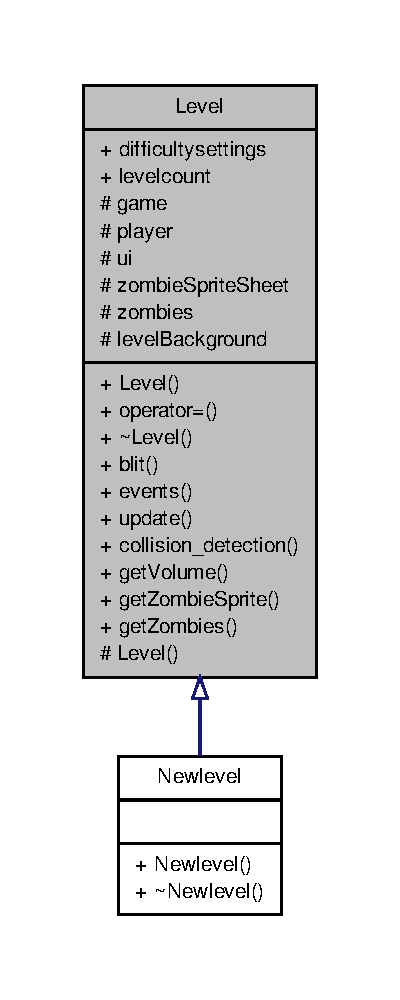
\includegraphics[width=192pt]{classLevel__inherit__graph}
\end{center}
\end{figure}


Collaboration diagram for Level\-:
\nopagebreak
\begin{figure}[H]
\begin{center}
\leavevmode
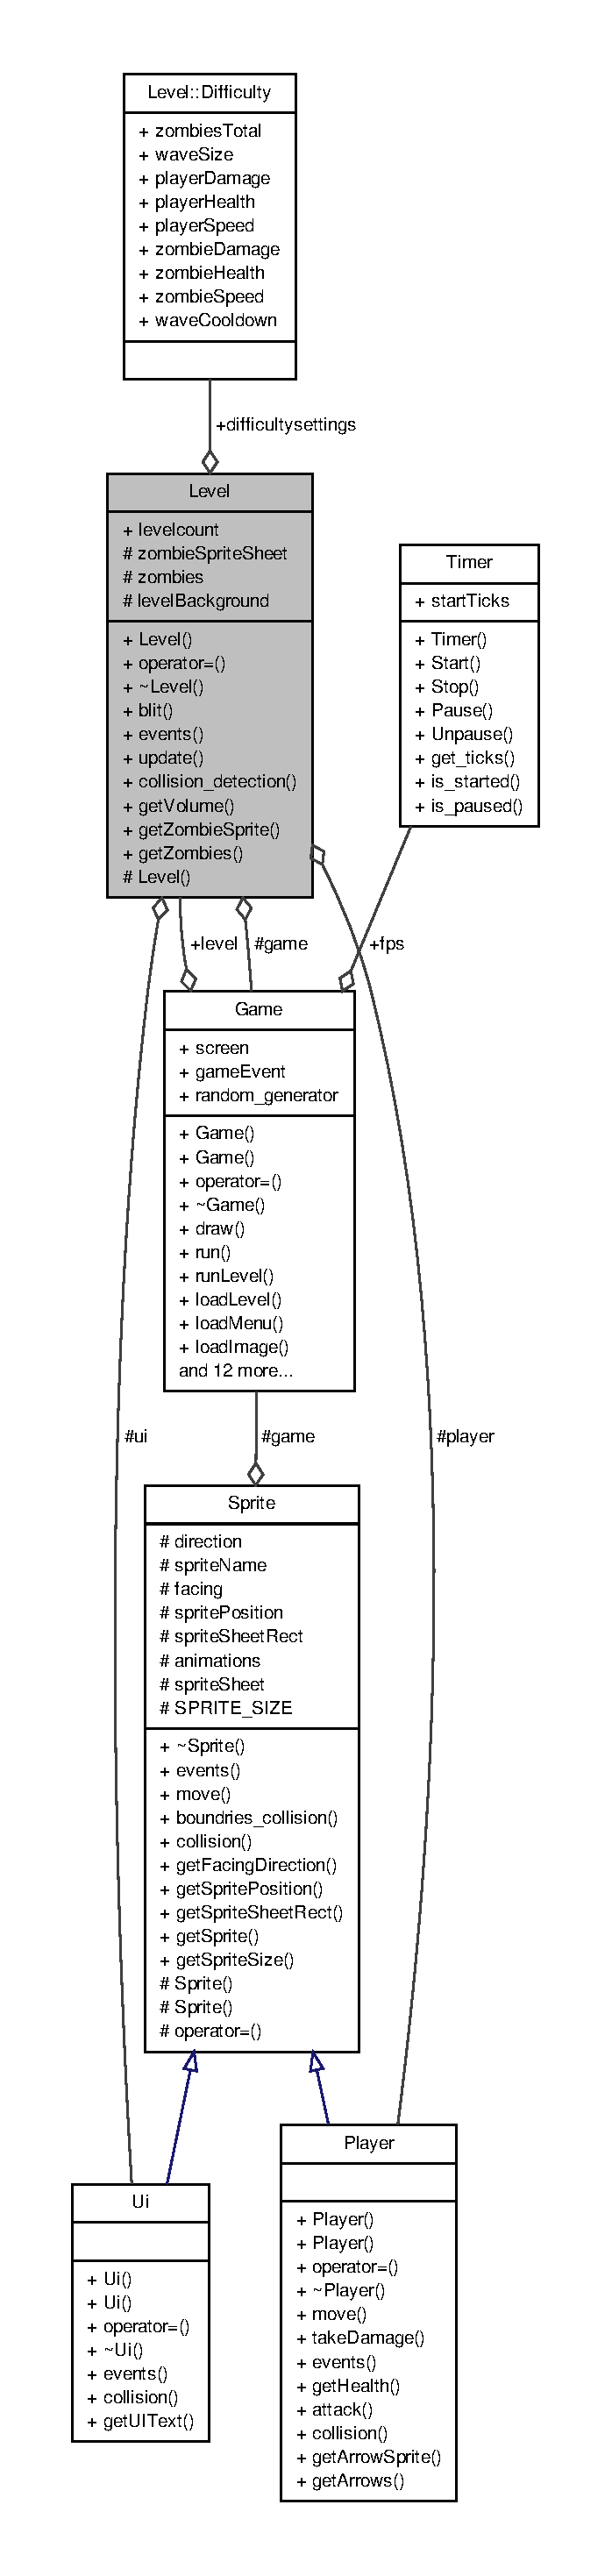
\includegraphics[height=550pt]{classLevel__coll__graph}
\end{center}
\end{figure}
\subsection*{Classes}
\begin{DoxyCompactItemize}
\item 
struct \hyperlink{structLevel_1_1Difficulty}{Difficulty}
\end{DoxyCompactItemize}
\subsection*{Public Member Functions}
\begin{DoxyCompactItemize}
\item 
\hyperlink{classLevel_ae03636cc90bd5f178650bd366124cb1c}{Level} (const \hyperlink{classLevel}{Level} \&)=delete
\item 
\hyperlink{classLevel}{Level} \& \hyperlink{classLevel_acbd996c953d3e3436cafddbf476cdba0}{operator=} (const \hyperlink{classLevel}{Level} \&)=delete
\item 
virtual \hyperlink{classLevel_a249eac1e8f19ff44134efa5e986feaca}{$\sim$\-Level} ()
\item 
void \hyperlink{classLevel_aa1f4afede83296a5f90254a1b8c558f3}{blit} ()
\item 
void \hyperlink{classLevel_a099ff502ab97a3c8bcf8511690d734d8}{events} ()
\item 
void \hyperlink{classLevel_a62e412eaad753d2baa2f94239cb80e41}{update} ()
\item 
void \hyperlink{classLevel_a44653e86f4db052e42396b0d4e95cc0a}{collision\-\_\-detection} ()
\item 
int \hyperlink{classLevel_aaf2eebf04cd6fe9343df05d7bd758119}{get\-Volume} ()
\item 
S\-D\-L\-\_\-\-Surface $\ast$ \hyperlink{classLevel_aab6e60626fa71aa9db1161ade94ca442}{get\-Zombie\-Sprite} () const 
\item 
std\-::list$<$ \hyperlink{classZombie}{Zombie} $\ast$ $>$ \& \hyperlink{classLevel_a11472360cfb4e4c6984015d86b5f7a96}{get\-Zombies} ()
\end{DoxyCompactItemize}
\subsection*{Public Attributes}
\begin{DoxyCompactItemize}
\item 
\hyperlink{structLevel_1_1Difficulty}{Difficulty} \hyperlink{classLevel_a940e0830c532595cc4509be6f68f30b9}{difficultysettings}
\end{DoxyCompactItemize}
\subsection*{Static Public Attributes}
\begin{DoxyCompactItemize}
\item 
static int \hyperlink{classLevel_a1af089e10ff0fc446d57277d48709622}{levelcount} = 0
\end{DoxyCompactItemize}
\subsection*{Protected Member Functions}
\begin{DoxyCompactItemize}
\item 
\hyperlink{classLevel_a0af6f93b99224d07a5eefb0c73df20b1}{Level} (\hyperlink{classGame}{Game} $\ast$game\-Pointer)
\end{DoxyCompactItemize}
\subsection*{Protected Attributes}
\begin{DoxyCompactItemize}
\item 
\hyperlink{classGame}{Game} $\ast$ \hyperlink{classLevel_acefd7bcf714862644a1c7f6ab0462fe4}{game}
\item 
\hyperlink{classPlayer}{Player} $\ast$ \hyperlink{classLevel_a76b010ccc524cef1ae0c3adc2a63d3b1}{player} \{nullptr\}
\item 
\hyperlink{classUi}{Ui} $\ast$ \hyperlink{classLevel_aefdedc06660278bcea9e0d06460af308}{ui} \{nullptr\}
\item 
S\-D\-L\-\_\-\-Surface $\ast$ \hyperlink{classLevel_af0f53f17e06a467013d4612c13bbdc68}{zombie\-Sprite\-Sheet} \{nullptr\}
\item 
std\-::list$<$ \hyperlink{classZombie}{Zombie} $\ast$ $>$ \hyperlink{classLevel_a507f4b9bc3a1b4acf67c8857a942f584}{zombies} \{\}
\item 
S\-D\-L\-\_\-\-Surface $\ast$ \hyperlink{classLevel_a0016c5498bfdf767cf58bd36d5b1e8c0}{level\-Background} \{nullptr\}
\end{DoxyCompactItemize}


\subsection{Constructor \& Destructor Documentation}
\hypertarget{classLevel_ae03636cc90bd5f178650bd366124cb1c}{\index{Level@{Level}!Level@{Level}}
\index{Level@{Level}!Level@{Level}}
\subsubsection[{Level}]{\setlength{\rightskip}{0pt plus 5cm}Level\-::\-Level (
\begin{DoxyParamCaption}
\item[{const {\bf Level} \&}]{}
\end{DoxyParamCaption}
)\hspace{0.3cm}{\ttfamily [delete]}}}\label{classLevel_ae03636cc90bd5f178650bd366124cb1c}
\hypertarget{classLevel_a249eac1e8f19ff44134efa5e986feaca}{\index{Level@{Level}!$\sim$\-Level@{$\sim$\-Level}}
\index{$\sim$\-Level@{$\sim$\-Level}!Level@{Level}}
\subsubsection[{$\sim$\-Level}]{\setlength{\rightskip}{0pt plus 5cm}Level\-::$\sim$\-Level (
\begin{DoxyParamCaption}
{}
\end{DoxyParamCaption}
)\hspace{0.3cm}{\ttfamily [virtual]}}}\label{classLevel_a249eac1e8f19ff44134efa5e986feaca}
level is resposible for freeing its surfaces and music.\hypertarget{classLevel_a0af6f93b99224d07a5eefb0c73df20b1}{\index{Level@{Level}!Level@{Level}}
\index{Level@{Level}!Level@{Level}}
\subsubsection[{Level}]{\setlength{\rightskip}{0pt plus 5cm}Level\-::\-Level (
\begin{DoxyParamCaption}
\item[{{\bf Game} $\ast$}]{game\-Pointer}
\end{DoxyParamCaption}
)\hspace{0.3cm}{\ttfamily [protected]}}}\label{classLevel_a0af6f93b99224d07a5eefb0c73df20b1}
level constructor loads the game music, sets the initial volume and increases that static counter level count by one. It loads the zombie sprite sheet, and stores the game \char`\"{}engine\char`\"{} pointer internally.

\subsection{Member Function Documentation}
\hypertarget{classLevel_aa1f4afede83296a5f90254a1b8c558f3}{\index{Level@{Level}!blit@{blit}}
\index{blit@{blit}!Level@{Level}}
\subsubsection[{blit}]{\setlength{\rightskip}{0pt plus 5cm}void Level\-::blit (
\begin{DoxyParamCaption}
{}
\end{DoxyParamCaption}
)}}\label{classLevel_aa1f4afede83296a5f90254a1b8c558f3}
blit will draw the level, arrows, zombies and the user interface.\hypertarget{classLevel_a44653e86f4db052e42396b0d4e95cc0a}{\index{Level@{Level}!collision\-\_\-detection@{collision\-\_\-detection}}
\index{collision\-\_\-detection@{collision\-\_\-detection}!Level@{Level}}
\subsubsection[{collision\-\_\-detection}]{\setlength{\rightskip}{0pt plus 5cm}void Level\-::collision\-\_\-detection (
\begin{DoxyParamCaption}
{}
\end{DoxyParamCaption}
)}}\label{classLevel_a44653e86f4db052e42396b0d4e95cc0a}
every type of movable object has to stay inside the screen area so we call boundry collisions and each objects own collision detection functions to determine what action to take when objects collide with walls or other objects.

Check the players arrows for any collisions with boundries or enemies\hypertarget{classLevel_a099ff502ab97a3c8bcf8511690d734d8}{\index{Level@{Level}!events@{events}}
\index{events@{events}!Level@{Level}}
\subsubsection[{events}]{\setlength{\rightskip}{0pt plus 5cm}void Level\-::events (
\begin{DoxyParamCaption}
{}
\end{DoxyParamCaption}
)}}\label{classLevel_a099ff502ab97a3c8bcf8511690d734d8}
events goes through every object in the level and checks each objects own events. it handles spawning of zombies, updating health, etc.

Checks that we havn't reached max amout of zombies spawned and spawns a wave of zombies every x seconds\hypertarget{classLevel_aaf2eebf04cd6fe9343df05d7bd758119}{\index{Level@{Level}!get\-Volume@{get\-Volume}}
\index{get\-Volume@{get\-Volume}!Level@{Level}}
\subsubsection[{get\-Volume}]{\setlength{\rightskip}{0pt plus 5cm}int Level\-::get\-Volume (
\begin{DoxyParamCaption}
{}
\end{DoxyParamCaption}
)}}\label{classLevel_aaf2eebf04cd6fe9343df05d7bd758119}
\hypertarget{classLevel_a11472360cfb4e4c6984015d86b5f7a96}{\index{Level@{Level}!get\-Zombies@{get\-Zombies}}
\index{get\-Zombies@{get\-Zombies}!Level@{Level}}
\subsubsection[{get\-Zombies}]{\setlength{\rightskip}{0pt plus 5cm}std\-::list$<$ {\bf Zombie} $\ast$ $>$ \& Level\-::get\-Zombies (
\begin{DoxyParamCaption}
{}
\end{DoxyParamCaption}
)}}\label{classLevel_a11472360cfb4e4c6984015d86b5f7a96}
returns a list of zombies that exist in-\/game.\hypertarget{classLevel_aab6e60626fa71aa9db1161ade94ca442}{\index{Level@{Level}!get\-Zombie\-Sprite@{get\-Zombie\-Sprite}}
\index{get\-Zombie\-Sprite@{get\-Zombie\-Sprite}!Level@{Level}}
\subsubsection[{get\-Zombie\-Sprite}]{\setlength{\rightskip}{0pt plus 5cm}S\-D\-L\-\_\-\-Surface $\ast$ Level\-::get\-Zombie\-Sprite (
\begin{DoxyParamCaption}
{}
\end{DoxyParamCaption}
) const}}\label{classLevel_aab6e60626fa71aa9db1161ade94ca442}
returns the zombie sprite\hypertarget{classLevel_acbd996c953d3e3436cafddbf476cdba0}{\index{Level@{Level}!operator=@{operator=}}
\index{operator=@{operator=}!Level@{Level}}
\subsubsection[{operator=}]{\setlength{\rightskip}{0pt plus 5cm}{\bf Level}\& Level\-::operator= (
\begin{DoxyParamCaption}
\item[{const {\bf Level} \&}]{}
\end{DoxyParamCaption}
)\hspace{0.3cm}{\ttfamily [delete]}}}\label{classLevel_acbd996c953d3e3436cafddbf476cdba0}
\hypertarget{classLevel_a62e412eaad753d2baa2f94239cb80e41}{\index{Level@{Level}!update@{update}}
\index{update@{update}!Level@{Level}}
\subsubsection[{update}]{\setlength{\rightskip}{0pt plus 5cm}void Level\-::update (
\begin{DoxyParamCaption}
{}
\end{DoxyParamCaption}
)}}\label{classLevel_a62e412eaad753d2baa2f94239cb80e41}
update does the actual moving of all objects on screen it moves the player, arrows, zombies and everything else that is moving.

\subsection{Member Data Documentation}
\hypertarget{classLevel_a940e0830c532595cc4509be6f68f30b9}{\index{Level@{Level}!difficultysettings@{difficultysettings}}
\index{difficultysettings@{difficultysettings}!Level@{Level}}
\subsubsection[{difficultysettings}]{\setlength{\rightskip}{0pt plus 5cm}{\bf Difficulty} Level\-::difficultysettings}}\label{classLevel_a940e0830c532595cc4509be6f68f30b9}
\hypertarget{classLevel_acefd7bcf714862644a1c7f6ab0462fe4}{\index{Level@{Level}!game@{game}}
\index{game@{game}!Level@{Level}}
\subsubsection[{game}]{\setlength{\rightskip}{0pt plus 5cm}{\bf Game}$\ast$ Level\-::game\hspace{0.3cm}{\ttfamily [protected]}}}\label{classLevel_acefd7bcf714862644a1c7f6ab0462fe4}
\hypertarget{classLevel_a0016c5498bfdf767cf58bd36d5b1e8c0}{\index{Level@{Level}!level\-Background@{level\-Background}}
\index{level\-Background@{level\-Background}!Level@{Level}}
\subsubsection[{level\-Background}]{\setlength{\rightskip}{0pt plus 5cm}S\-D\-L\-\_\-\-Surface$\ast$ Level\-::level\-Background \{nullptr\}\hspace{0.3cm}{\ttfamily [protected]}}}\label{classLevel_a0016c5498bfdf767cf58bd36d5b1e8c0}
\hypertarget{classLevel_a1af089e10ff0fc446d57277d48709622}{\index{Level@{Level}!levelcount@{levelcount}}
\index{levelcount@{levelcount}!Level@{Level}}
\subsubsection[{levelcount}]{\setlength{\rightskip}{0pt plus 5cm}int Level\-::levelcount = 0\hspace{0.3cm}{\ttfamily [static]}}}\label{classLevel_a1af089e10ff0fc446d57277d48709622}
\hypertarget{classLevel_a76b010ccc524cef1ae0c3adc2a63d3b1}{\index{Level@{Level}!player@{player}}
\index{player@{player}!Level@{Level}}
\subsubsection[{player}]{\setlength{\rightskip}{0pt plus 5cm}{\bf Player}$\ast$ Level\-::player \{nullptr\}\hspace{0.3cm}{\ttfamily [protected]}}}\label{classLevel_a76b010ccc524cef1ae0c3adc2a63d3b1}
\hypertarget{classLevel_aefdedc06660278bcea9e0d06460af308}{\index{Level@{Level}!ui@{ui}}
\index{ui@{ui}!Level@{Level}}
\subsubsection[{ui}]{\setlength{\rightskip}{0pt plus 5cm}{\bf Ui}$\ast$ Level\-::ui \{nullptr\}\hspace{0.3cm}{\ttfamily [protected]}}}\label{classLevel_aefdedc06660278bcea9e0d06460af308}
\hypertarget{classLevel_a507f4b9bc3a1b4acf67c8857a942f584}{\index{Level@{Level}!zombies@{zombies}}
\index{zombies@{zombies}!Level@{Level}}
\subsubsection[{zombies}]{\setlength{\rightskip}{0pt plus 5cm}std\-::list$<${\bf Zombie}$\ast$$>$ Level\-::zombies \{\}\hspace{0.3cm}{\ttfamily [protected]}}}\label{classLevel_a507f4b9bc3a1b4acf67c8857a942f584}
\hypertarget{classLevel_af0f53f17e06a467013d4612c13bbdc68}{\index{Level@{Level}!zombie\-Sprite\-Sheet@{zombie\-Sprite\-Sheet}}
\index{zombie\-Sprite\-Sheet@{zombie\-Sprite\-Sheet}!Level@{Level}}
\subsubsection[{zombie\-Sprite\-Sheet}]{\setlength{\rightskip}{0pt plus 5cm}S\-D\-L\-\_\-\-Surface$\ast$ Level\-::zombie\-Sprite\-Sheet \{nullptr\}\hspace{0.3cm}{\ttfamily [protected]}}}\label{classLevel_af0f53f17e06a467013d4612c13bbdc68}


The documentation for this class was generated from the following files\-:\begin{DoxyCompactItemize}
\item 
\hyperlink{level_8h}{level.\-h}\item 
\hyperlink{level_8cc}{level.\-cc}\end{DoxyCompactItemize}

\hypertarget{classMenu}{\section{Menu Class Reference}
\label{classMenu}\index{Menu@{Menu}}
}


{\ttfamily \#include $<$menu.\-h$>$}



Collaboration diagram for Menu\-:\nopagebreak
\begin{figure}[H]
\begin{center}
\leavevmode
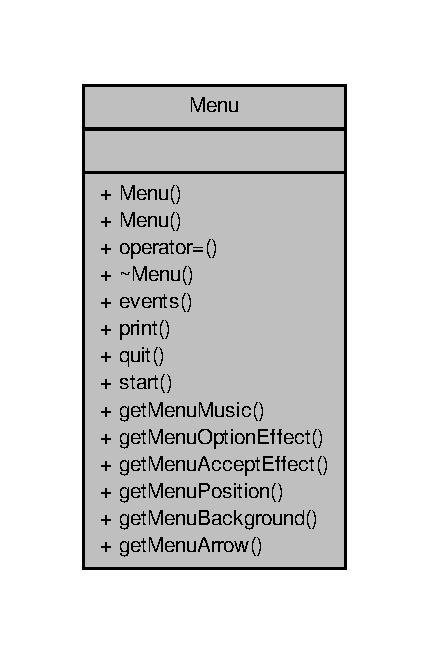
\includegraphics[width=206pt]{classMenu__coll__graph}
\end{center}
\end{figure}
\subsection*{Public Member Functions}
\begin{DoxyCompactItemize}
\item 
\hyperlink{classMenu_a91ec4975ad2aced80cd524a179dd7af1}{Menu} (\hyperlink{classGame}{Game} $\ast$game)
\item 
\hyperlink{classMenu_a63ab2f09293dba94a040e7303c069f5e}{Menu} (const \hyperlink{classMenu}{Menu} \&)=delete
\item 
\hyperlink{classMenu}{Menu} \& \hyperlink{classMenu_a2d63d2845c50e44eaf960876374f436a}{operator=} (const \hyperlink{classMenu}{Menu} \&)=delete
\item 
\hyperlink{classMenu_a831387f51358cfb88cd018e1777bc980}{$\sim$\-Menu} ()
\item 
void \hyperlink{classMenu_ac608f2d42a24c44578f3817218a36767}{events} ()
\item 
void \hyperlink{classMenu_aa6ff784314cc009478562d9ab7a0af34}{print} ()
\item 
void \hyperlink{classMenu_a5072c4d7aca8f9071c9ee9025a7019f9}{quit} ()
\item 
void \hyperlink{classMenu_ae1ec62e738dda7faaaec850bd0b58ffe}{start} ()
\item 
Mix\-\_\-\-Music $\ast$ \hyperlink{classMenu_a85a656aa9531a1308b5251c8f9df4cf3}{get\-Menu\-Music} () const 
\item 
Mix\-\_\-\-Chunk $\ast$ \hyperlink{classMenu_a9df0489e11835af740aa631ded1f1c07}{get\-Menu\-Option\-Effect} () const 
\item 
Mix\-\_\-\-Chunk $\ast$ \hyperlink{classMenu_a83ed1717ee5a549941e842f3250ca546}{get\-Menu\-Accept\-Effect} () const 
\item 
const S\-D\-L\-\_\-\-Rect \& \hyperlink{classMenu_a736db9878b209cde78a9ecd55e1adf11}{get\-Menu\-Position} () const 
\item 
S\-D\-L\-\_\-\-Surface $\ast$ \hyperlink{classMenu_adf2daad60f2175d887d8592998261c9a}{get\-Menu\-Background} () const 
\item 
S\-D\-L\-\_\-\-Surface $\ast$ \hyperlink{classMenu_a2e4f4c37e121c7446db8bb5ee2a214bc}{get\-Menu\-Arrow} () const 
\end{DoxyCompactItemize}


\subsection{Constructor \& Destructor Documentation}
\hypertarget{classMenu_a91ec4975ad2aced80cd524a179dd7af1}{\index{Menu@{Menu}!Menu@{Menu}}
\index{Menu@{Menu}!Menu@{Menu}}
\subsubsection[{Menu}]{\setlength{\rightskip}{0pt plus 5cm}Menu\-::\-Menu (
\begin{DoxyParamCaption}
\item[{{\bf Game} $\ast$}]{game}
\end{DoxyParamCaption}
)}}\label{classMenu_a91ec4975ad2aced80cd524a179dd7af1}
the menu constructor loads all menu images, music and also sets the default option in the game menu.\hypertarget{classMenu_a63ab2f09293dba94a040e7303c069f5e}{\index{Menu@{Menu}!Menu@{Menu}}
\index{Menu@{Menu}!Menu@{Menu}}
\subsubsection[{Menu}]{\setlength{\rightskip}{0pt plus 5cm}Menu\-::\-Menu (
\begin{DoxyParamCaption}
\item[{const {\bf Menu} \&}]{}
\end{DoxyParamCaption}
)\hspace{0.3cm}{\ttfamily [delete]}}}\label{classMenu_a63ab2f09293dba94a040e7303c069f5e}
\hypertarget{classMenu_a831387f51358cfb88cd018e1777bc980}{\index{Menu@{Menu}!$\sim$\-Menu@{$\sim$\-Menu}}
\index{$\sim$\-Menu@{$\sim$\-Menu}!Menu@{Menu}}
\subsubsection[{$\sim$\-Menu}]{\setlength{\rightskip}{0pt plus 5cm}Menu\-::$\sim$\-Menu (
\begin{DoxyParamCaption}
{}
\end{DoxyParamCaption}
)}}\label{classMenu_a831387f51358cfb88cd018e1777bc980}
menu is responsible for freeing its surfaces and music.

\subsection{Member Function Documentation}
\hypertarget{classMenu_ac608f2d42a24c44578f3817218a36767}{\index{Menu@{Menu}!events@{events}}
\index{events@{events}!Menu@{Menu}}
\subsubsection[{events}]{\setlength{\rightskip}{0pt plus 5cm}void Menu\-::events (
\begin{DoxyParamCaption}
{}
\end{DoxyParamCaption}
)}}\label{classMenu_ac608f2d42a24c44578f3817218a36767}
handles the menu events, such as moving up / down in the menu and choosing either start or exit.\hypertarget{classMenu_a83ed1717ee5a549941e842f3250ca546}{\index{Menu@{Menu}!get\-Menu\-Accept\-Effect@{get\-Menu\-Accept\-Effect}}
\index{get\-Menu\-Accept\-Effect@{get\-Menu\-Accept\-Effect}!Menu@{Menu}}
\subsubsection[{get\-Menu\-Accept\-Effect}]{\setlength{\rightskip}{0pt plus 5cm}Mix\-\_\-\-Chunk $\ast$ Menu\-::get\-Menu\-Accept\-Effect (
\begin{DoxyParamCaption}
{}
\end{DoxyParamCaption}
) const}}\label{classMenu_a83ed1717ee5a549941e842f3250ca546}
returns the sound effect when choosing a menu option.\hypertarget{classMenu_a2e4f4c37e121c7446db8bb5ee2a214bc}{\index{Menu@{Menu}!get\-Menu\-Arrow@{get\-Menu\-Arrow}}
\index{get\-Menu\-Arrow@{get\-Menu\-Arrow}!Menu@{Menu}}
\subsubsection[{get\-Menu\-Arrow}]{\setlength{\rightskip}{0pt plus 5cm}S\-D\-L\-\_\-\-Surface $\ast$ Menu\-::get\-Menu\-Arrow (
\begin{DoxyParamCaption}
{}
\end{DoxyParamCaption}
) const}}\label{classMenu_a2e4f4c37e121c7446db8bb5ee2a214bc}
returns the surface of the menu arrow.\hypertarget{classMenu_adf2daad60f2175d887d8592998261c9a}{\index{Menu@{Menu}!get\-Menu\-Background@{get\-Menu\-Background}}
\index{get\-Menu\-Background@{get\-Menu\-Background}!Menu@{Menu}}
\subsubsection[{get\-Menu\-Background}]{\setlength{\rightskip}{0pt plus 5cm}S\-D\-L\-\_\-\-Surface $\ast$ Menu\-::get\-Menu\-Background (
\begin{DoxyParamCaption}
{}
\end{DoxyParamCaption}
) const}}\label{classMenu_adf2daad60f2175d887d8592998261c9a}
returns the surface of the menu background.\hypertarget{classMenu_a85a656aa9531a1308b5251c8f9df4cf3}{\index{Menu@{Menu}!get\-Menu\-Music@{get\-Menu\-Music}}
\index{get\-Menu\-Music@{get\-Menu\-Music}!Menu@{Menu}}
\subsubsection[{get\-Menu\-Music}]{\setlength{\rightskip}{0pt plus 5cm}Mix\-\_\-\-Music $\ast$ Menu\-::get\-Menu\-Music (
\begin{DoxyParamCaption}
{}
\end{DoxyParamCaption}
) const}}\label{classMenu_a85a656aa9531a1308b5251c8f9df4cf3}
returns the menu music.\hypertarget{classMenu_a9df0489e11835af740aa631ded1f1c07}{\index{Menu@{Menu}!get\-Menu\-Option\-Effect@{get\-Menu\-Option\-Effect}}
\index{get\-Menu\-Option\-Effect@{get\-Menu\-Option\-Effect}!Menu@{Menu}}
\subsubsection[{get\-Menu\-Option\-Effect}]{\setlength{\rightskip}{0pt plus 5cm}Mix\-\_\-\-Chunk $\ast$ Menu\-::get\-Menu\-Option\-Effect (
\begin{DoxyParamCaption}
{}
\end{DoxyParamCaption}
) const}}\label{classMenu_a9df0489e11835af740aa631ded1f1c07}
returns the sound effect when switching menu option.\hypertarget{classMenu_a736db9878b209cde78a9ecd55e1adf11}{\index{Menu@{Menu}!get\-Menu\-Position@{get\-Menu\-Position}}
\index{get\-Menu\-Position@{get\-Menu\-Position}!Menu@{Menu}}
\subsubsection[{get\-Menu\-Position}]{\setlength{\rightskip}{0pt plus 5cm}const S\-D\-L\-\_\-\-Rect \& Menu\-::get\-Menu\-Position (
\begin{DoxyParamCaption}
{}
\end{DoxyParamCaption}
) const}}\label{classMenu_a736db9878b209cde78a9ecd55e1adf11}
gets the current position in the menu (the menu arrow).\hypertarget{classMenu_a2d63d2845c50e44eaf960876374f436a}{\index{Menu@{Menu}!operator=@{operator=}}
\index{operator=@{operator=}!Menu@{Menu}}
\subsubsection[{operator=}]{\setlength{\rightskip}{0pt plus 5cm}{\bf Menu}\& Menu\-::operator= (
\begin{DoxyParamCaption}
\item[{const {\bf Menu} \&}]{}
\end{DoxyParamCaption}
)\hspace{0.3cm}{\ttfamily [delete]}}}\label{classMenu_a2d63d2845c50e44eaf960876374f436a}
\hypertarget{classMenu_aa6ff784314cc009478562d9ab7a0af34}{\index{Menu@{Menu}!print@{print}}
\index{print@{print}!Menu@{Menu}}
\subsubsection[{print}]{\setlength{\rightskip}{0pt plus 5cm}void Menu\-::print (
\begin{DoxyParamCaption}
{}
\end{DoxyParamCaption}
)}}\label{classMenu_aa6ff784314cc009478562d9ab7a0af34}
\hypertarget{classMenu_a5072c4d7aca8f9071c9ee9025a7019f9}{\index{Menu@{Menu}!quit@{quit}}
\index{quit@{quit}!Menu@{Menu}}
\subsubsection[{quit}]{\setlength{\rightskip}{0pt plus 5cm}void Menu\-::quit (
\begin{DoxyParamCaption}
{}
\end{DoxyParamCaption}
)}}\label{classMenu_a5072c4d7aca8f9071c9ee9025a7019f9}
updates the games state to its exit-\/state.\hypertarget{classMenu_ae1ec62e738dda7faaaec850bd0b58ffe}{\index{Menu@{Menu}!start@{start}}
\index{start@{start}!Menu@{Menu}}
\subsubsection[{start}]{\setlength{\rightskip}{0pt plus 5cm}void Menu\-::start (
\begin{DoxyParamCaption}
{}
\end{DoxyParamCaption}
)}}\label{classMenu_ae1ec62e738dda7faaaec850bd0b58ffe}
updates the games state to its play-\/state.

The documentation for this class was generated from the following files\-:\begin{DoxyCompactItemize}
\item 
\hyperlink{menu_8h}{menu.\-h}\item 
\hyperlink{menu_8cc}{menu.\-cc}\end{DoxyCompactItemize}

\hypertarget{classNewlevel}{\section{Newlevel Class Reference}
\label{classNewlevel}\index{Newlevel@{Newlevel}}
}


{\ttfamily \#include $<$newlevel.\-h$>$}



Inheritance diagram for Newlevel\-:\nopagebreak
\begin{figure}[H]
\begin{center}
\leavevmode
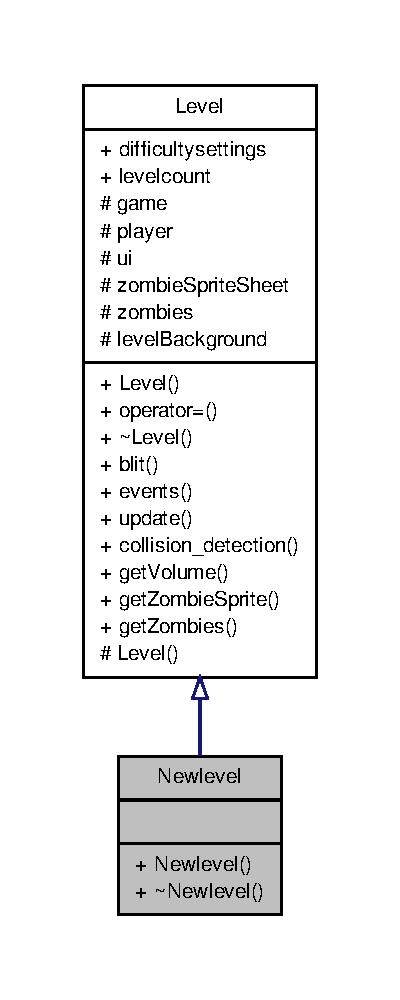
\includegraphics[width=192pt]{classNewlevel__inherit__graph}
\end{center}
\end{figure}


Collaboration diagram for Newlevel\-:
\nopagebreak
\begin{figure}[H]
\begin{center}
\leavevmode
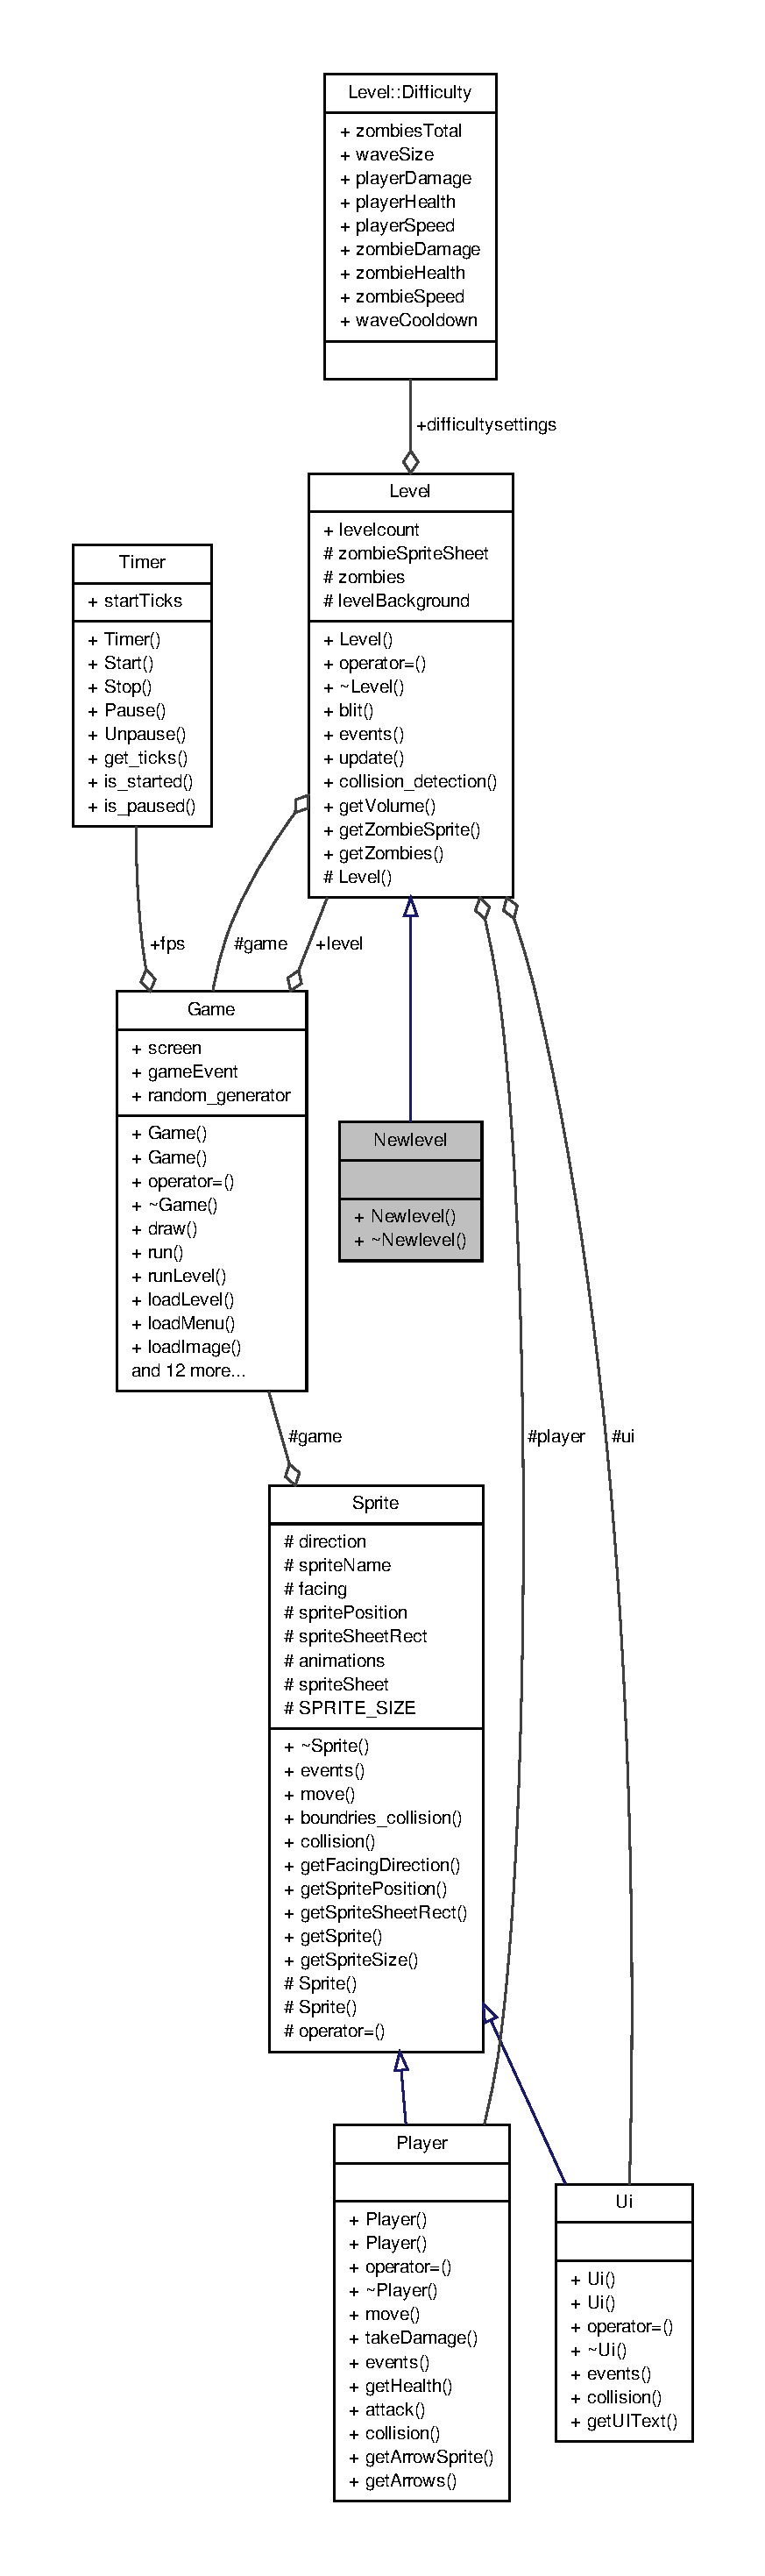
\includegraphics[height=550pt]{classNewlevel__coll__graph}
\end{center}
\end{figure}
\subsection*{Public Member Functions}
\begin{DoxyCompactItemize}
\item 
\hyperlink{classNewlevel_a677e40755e35f100d2a3ab7890b76a94}{Newlevel} (\hyperlink{classGame}{Game} $\ast$game\-Pointer)
\item 
\hyperlink{classNewlevel_a552bd423d5925e29a0555bde2d1ac7a6}{$\sim$\-Newlevel} ()
\end{DoxyCompactItemize}
\subsection*{Additional Inherited Members}


\subsection{Constructor \& Destructor Documentation}
\hypertarget{classNewlevel_a677e40755e35f100d2a3ab7890b76a94}{\index{Newlevel@{Newlevel}!Newlevel@{Newlevel}}
\index{Newlevel@{Newlevel}!Newlevel@{Newlevel}}
\subsubsection[{Newlevel}]{\setlength{\rightskip}{0pt plus 5cm}Newlevel\-::\-Newlevel (
\begin{DoxyParamCaption}
\item[{{\bf Game} $\ast$}]{game\-Pointer}
\end{DoxyParamCaption}
)}}\label{classNewlevel_a677e40755e35f100d2a3ab7890b76a94}
\hypertarget{classNewlevel_a552bd423d5925e29a0555bde2d1ac7a6}{\index{Newlevel@{Newlevel}!$\sim$\-Newlevel@{$\sim$\-Newlevel}}
\index{$\sim$\-Newlevel@{$\sim$\-Newlevel}!Newlevel@{Newlevel}}
\subsubsection[{$\sim$\-Newlevel}]{\setlength{\rightskip}{0pt plus 5cm}Newlevel\-::$\sim$\-Newlevel (
\begin{DoxyParamCaption}
{}
\end{DoxyParamCaption}
)}}\label{classNewlevel_a552bd423d5925e29a0555bde2d1ac7a6}


The documentation for this class was generated from the following files\-:\begin{DoxyCompactItemize}
\item 
\hyperlink{newlevel_8h}{newlevel.\-h}\item 
\hyperlink{newlevel_8cc}{newlevel.\-cc}\end{DoxyCompactItemize}

\hypertarget{classPlayer}{\section{Player Class Reference}
\label{classPlayer}\index{Player@{Player}}
}


{\ttfamily \#include $<$player.\-h$>$}



Inheritance diagram for Player\-:\nopagebreak
\begin{figure}[H]
\begin{center}
\leavevmode
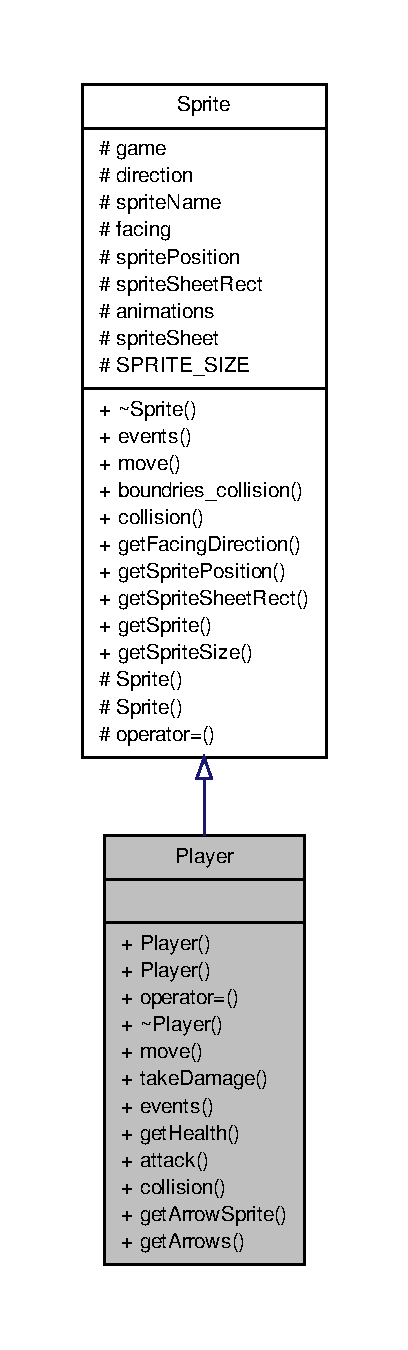
\includegraphics[height=550pt]{classPlayer__inherit__graph}
\end{center}
\end{figure}


Collaboration diagram for Player\-:
\nopagebreak
\begin{figure}[H]
\begin{center}
\leavevmode
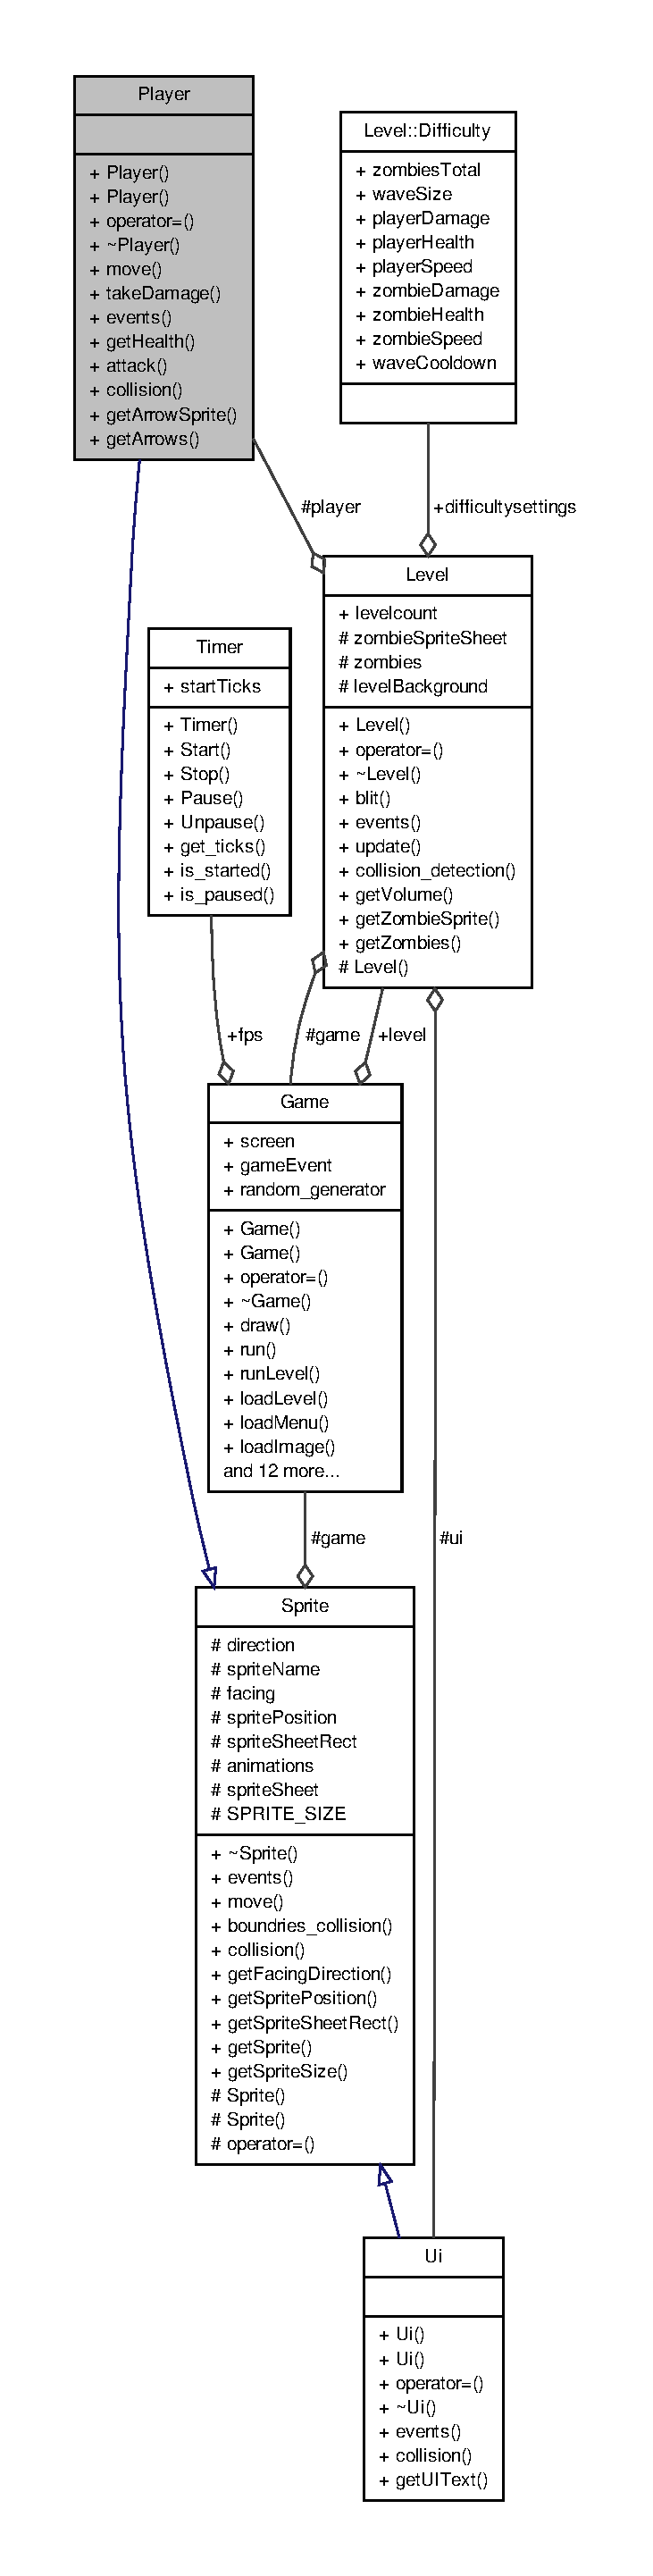
\includegraphics[height=550pt]{classPlayer__coll__graph}
\end{center}
\end{figure}
\subsection*{Public Member Functions}
\begin{DoxyCompactItemize}
\item 
\hyperlink{classPlayer_aa7539e1f537c97414963214a1dc1aa65}{Player} (\hyperlink{classGame}{Game} $\ast$game, \hyperlink{classLevel}{Level} $\ast$level, std\-::string playername)
\item 
\hyperlink{classPlayer_ae8015d1f08ba69d663cfdaea1a64d1a4}{Player} (const \hyperlink{classPlayer}{Player} \&)=delete
\item 
\hyperlink{classPlayer}{Player} \& \hyperlink{classPlayer_ab81d34e4adb4e329d26b1635d866462d}{operator=} (const \hyperlink{classPlayer}{Player} \&)=delete
\item 
\hyperlink{classPlayer_a749d2c00e1fe0f5c2746f7505a58c062}{$\sim$\-Player} ()
\item 
void \hyperlink{classPlayer_ae02ee46d8c20dd0697b975f935b09839}{move} ()
\item 
void \hyperlink{classPlayer_af97f9b32912f28fdcdad1785d515cd2d}{take\-Damage} (int damage)
\item 
void \hyperlink{classPlayer_a9df270c5655b433d057e3e0f8fafd9ae}{events} ()
\item 
int \hyperlink{classPlayer_abcb15d249bed9a4ab0ab86b52b0d747a}{get\-Health} ()
\item 
int \hyperlink{classPlayer_a8ce2d81f916ae4634459d7fccc232c23}{attack} ()
\item 
bool \hyperlink{classPlayer_a740c5163bb90b6b5824aed4817b0c2cc}{collision} ()
\item 
S\-D\-L\-\_\-\-Surface $\ast$ \hyperlink{classPlayer_a9a65f7260bffb2a72c68d8692f447a06}{get\-Arrow\-Sprite} () const 
\item 
std\-::list$<$ \hyperlink{classArrow}{Arrow} $\ast$ $>$ \& \hyperlink{classPlayer_a9282a44ce22f9192413326f26459a7e4}{get\-Arrows} ()
\end{DoxyCompactItemize}
\subsection*{Additional Inherited Members}


\subsection{Constructor \& Destructor Documentation}
\hypertarget{classPlayer_aa7539e1f537c97414963214a1dc1aa65}{\index{Player@{Player}!Player@{Player}}
\index{Player@{Player}!Player@{Player}}
\subsubsection[{Player}]{\setlength{\rightskip}{0pt plus 5cm}Player\-::\-Player (
\begin{DoxyParamCaption}
\item[{{\bf Game} $\ast$}]{game, }
\item[{{\bf Level} $\ast$}]{level, }
\item[{std\-::string}]{playername}
\end{DoxyParamCaption}
)}}\label{classPlayer_aa7539e1f537c97414963214a1dc1aa65}
the player constructor loads the player sprite sheet, sets the size of the sprite, positions on the level, where in the sprite sheet the animation starts. It also sets the player health, damage and moving speed.\hypertarget{classPlayer_ae8015d1f08ba69d663cfdaea1a64d1a4}{\index{Player@{Player}!Player@{Player}}
\index{Player@{Player}!Player@{Player}}
\subsubsection[{Player}]{\setlength{\rightskip}{0pt plus 5cm}Player\-::\-Player (
\begin{DoxyParamCaption}
\item[{const {\bf Player} \&}]{}
\end{DoxyParamCaption}
)\hspace{0.3cm}{\ttfamily [delete]}}}\label{classPlayer_ae8015d1f08ba69d663cfdaea1a64d1a4}
\hypertarget{classPlayer_a749d2c00e1fe0f5c2746f7505a58c062}{\index{Player@{Player}!$\sim$\-Player@{$\sim$\-Player}}
\index{$\sim$\-Player@{$\sim$\-Player}!Player@{Player}}
\subsubsection[{$\sim$\-Player}]{\setlength{\rightskip}{0pt plus 5cm}Player\-::$\sim$\-Player (
\begin{DoxyParamCaption}
{}
\end{DoxyParamCaption}
)}}\label{classPlayer_a749d2c00e1fe0f5c2746f7505a58c062}
player is resposible for freeing its surfaces.

\subsection{Member Function Documentation}
\hypertarget{classPlayer_a8ce2d81f916ae4634459d7fccc232c23}{\index{Player@{Player}!attack@{attack}}
\index{attack@{attack}!Player@{Player}}
\subsubsection[{attack}]{\setlength{\rightskip}{0pt plus 5cm}int Player\-::attack (
\begin{DoxyParamCaption}
{}
\end{DoxyParamCaption}
)}}\label{classPlayer_a8ce2d81f916ae4634459d7fccc232c23}
attack deals damage equal to the players damage onto an enemy.\hypertarget{classPlayer_a740c5163bb90b6b5824aed4817b0c2cc}{\index{Player@{Player}!collision@{collision}}
\index{collision@{collision}!Player@{Player}}
\subsubsection[{collision}]{\setlength{\rightskip}{0pt plus 5cm}bool Player\-::collision (
\begin{DoxyParamCaption}
{}
\end{DoxyParamCaption}
)\hspace{0.3cm}{\ttfamily [virtual]}}}\label{classPlayer_a740c5163bb90b6b5824aed4817b0c2cc}
We check every zombie if we have collided with it, if we did we take damage and we also \char`\"{}bounce\char`\"{} back when we take damage, to show the player an effect of being attacked.

This part is so that we can be attacked even if we are standing still, meaning that the zombies direction is the primary focus in order to calculate how we should interact

Implements \hyperlink{classSprite_ae0c21af6a4fc7fb8e9daf72675a1ec50}{Sprite}.

\hypertarget{classPlayer_a9df270c5655b433d057e3e0f8fafd9ae}{\index{Player@{Player}!events@{events}}
\index{events@{events}!Player@{Player}}
\subsubsection[{events}]{\setlength{\rightskip}{0pt plus 5cm}void Player\-::events (
\begin{DoxyParamCaption}
{}
\end{DoxyParamCaption}
)\hspace{0.3cm}{\ttfamily [virtual]}}}\label{classPlayer_a9df270c5655b433d057e3e0f8fafd9ae}
this function handles our keypresses for moving, and also makes sure that we cant fire how many arrows we want, it limits our shooting speed to the allowed time interval.

If we press space then we shoot an arrow

if we have 0 hp, then we lost the game 

Reimplemented from \hyperlink{classSprite_a82cd02f494fe948457a8feb5ecd93212}{Sprite}.

\hypertarget{classPlayer_a9282a44ce22f9192413326f26459a7e4}{\index{Player@{Player}!get\-Arrows@{get\-Arrows}}
\index{get\-Arrows@{get\-Arrows}!Player@{Player}}
\subsubsection[{get\-Arrows}]{\setlength{\rightskip}{0pt plus 5cm}std\-::list$<$ {\bf Arrow} $\ast$ $>$ \& Player\-::get\-Arrows (
\begin{DoxyParamCaption}
{}
\end{DoxyParamCaption}
)}}\label{classPlayer_a9282a44ce22f9192413326f26459a7e4}
returns a list holding all of the arrows\hypertarget{classPlayer_a9a65f7260bffb2a72c68d8692f447a06}{\index{Player@{Player}!get\-Arrow\-Sprite@{get\-Arrow\-Sprite}}
\index{get\-Arrow\-Sprite@{get\-Arrow\-Sprite}!Player@{Player}}
\subsubsection[{get\-Arrow\-Sprite}]{\setlength{\rightskip}{0pt plus 5cm}S\-D\-L\-\_\-\-Surface $\ast$ Player\-::get\-Arrow\-Sprite (
\begin{DoxyParamCaption}
{}
\end{DoxyParamCaption}
) const}}\label{classPlayer_a9a65f7260bffb2a72c68d8692f447a06}
returns the surface holding the arrow sprite sheet.\hypertarget{classPlayer_abcb15d249bed9a4ab0ab86b52b0d747a}{\index{Player@{Player}!get\-Health@{get\-Health}}
\index{get\-Health@{get\-Health}!Player@{Player}}
\subsubsection[{get\-Health}]{\setlength{\rightskip}{0pt plus 5cm}int Player\-::get\-Health (
\begin{DoxyParamCaption}
{}
\end{DoxyParamCaption}
)}}\label{classPlayer_abcb15d249bed9a4ab0ab86b52b0d747a}
returns the players health.\hypertarget{classPlayer_ae02ee46d8c20dd0697b975f935b09839}{\index{Player@{Player}!move@{move}}
\index{move@{move}!Player@{Player}}
\subsubsection[{move}]{\setlength{\rightskip}{0pt plus 5cm}void Player\-::move (
\begin{DoxyParamCaption}
{}
\end{DoxyParamCaption}
)\hspace{0.3cm}{\ttfamily [virtual]}}}\label{classPlayer_ae02ee46d8c20dd0697b975f935b09839}
We use a system of direction with facing as our main way of telling the character how it should move when we have pressed certain buttons

Reimplemented from \hyperlink{classSprite_afcf196c3d93fd743fdcc6f84d128ece6}{Sprite}.

\hypertarget{classPlayer_ab81d34e4adb4e329d26b1635d866462d}{\index{Player@{Player}!operator=@{operator=}}
\index{operator=@{operator=}!Player@{Player}}
\subsubsection[{operator=}]{\setlength{\rightskip}{0pt plus 5cm}{\bf Player}\& Player\-::operator= (
\begin{DoxyParamCaption}
\item[{const {\bf Player} \&}]{}
\end{DoxyParamCaption}
)\hspace{0.3cm}{\ttfamily [delete]}}}\label{classPlayer_ab81d34e4adb4e329d26b1635d866462d}
\hypertarget{classPlayer_af97f9b32912f28fdcdad1785d515cd2d}{\index{Player@{Player}!take\-Damage@{take\-Damage}}
\index{take\-Damage@{take\-Damage}!Player@{Player}}
\subsubsection[{take\-Damage}]{\setlength{\rightskip}{0pt plus 5cm}void Player\-::take\-Damage (
\begin{DoxyParamCaption}
\item[{int}]{damage}
\end{DoxyParamCaption}
)}}\label{classPlayer_af97f9b32912f28fdcdad1785d515cd2d}
if we get hit we take damage equal to the damage taken.

The documentation for this class was generated from the following files\-:\begin{DoxyCompactItemize}
\item 
\hyperlink{player_8h}{player.\-h}\item 
\hyperlink{player_8cc}{player.\-cc}\end{DoxyCompactItemize}

\hypertarget{classSprite}{\section{Sprite Class Reference}
\label{classSprite}\index{Sprite@{Sprite}}
}


{\ttfamily \#include $<$sprite.\-h$>$}



Inheritance diagram for Sprite\-:\nopagebreak
\begin{figure}[H]
\begin{center}
\leavevmode
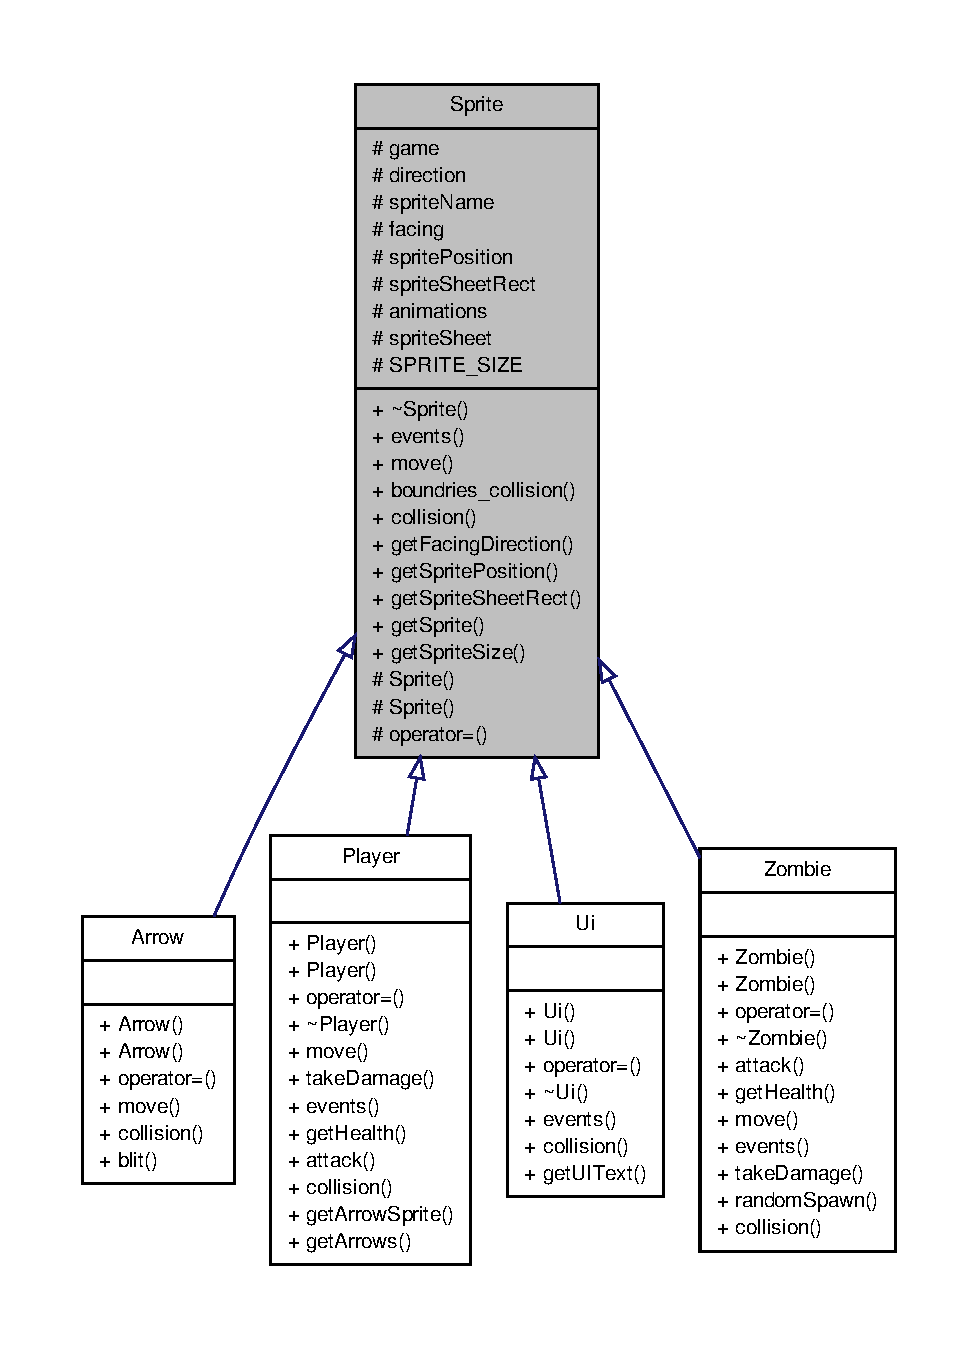
\includegraphics[width=350pt]{classSprite__inherit__graph}
\end{center}
\end{figure}


Collaboration diagram for Sprite\-:
\nopagebreak
\begin{figure}[H]
\begin{center}
\leavevmode
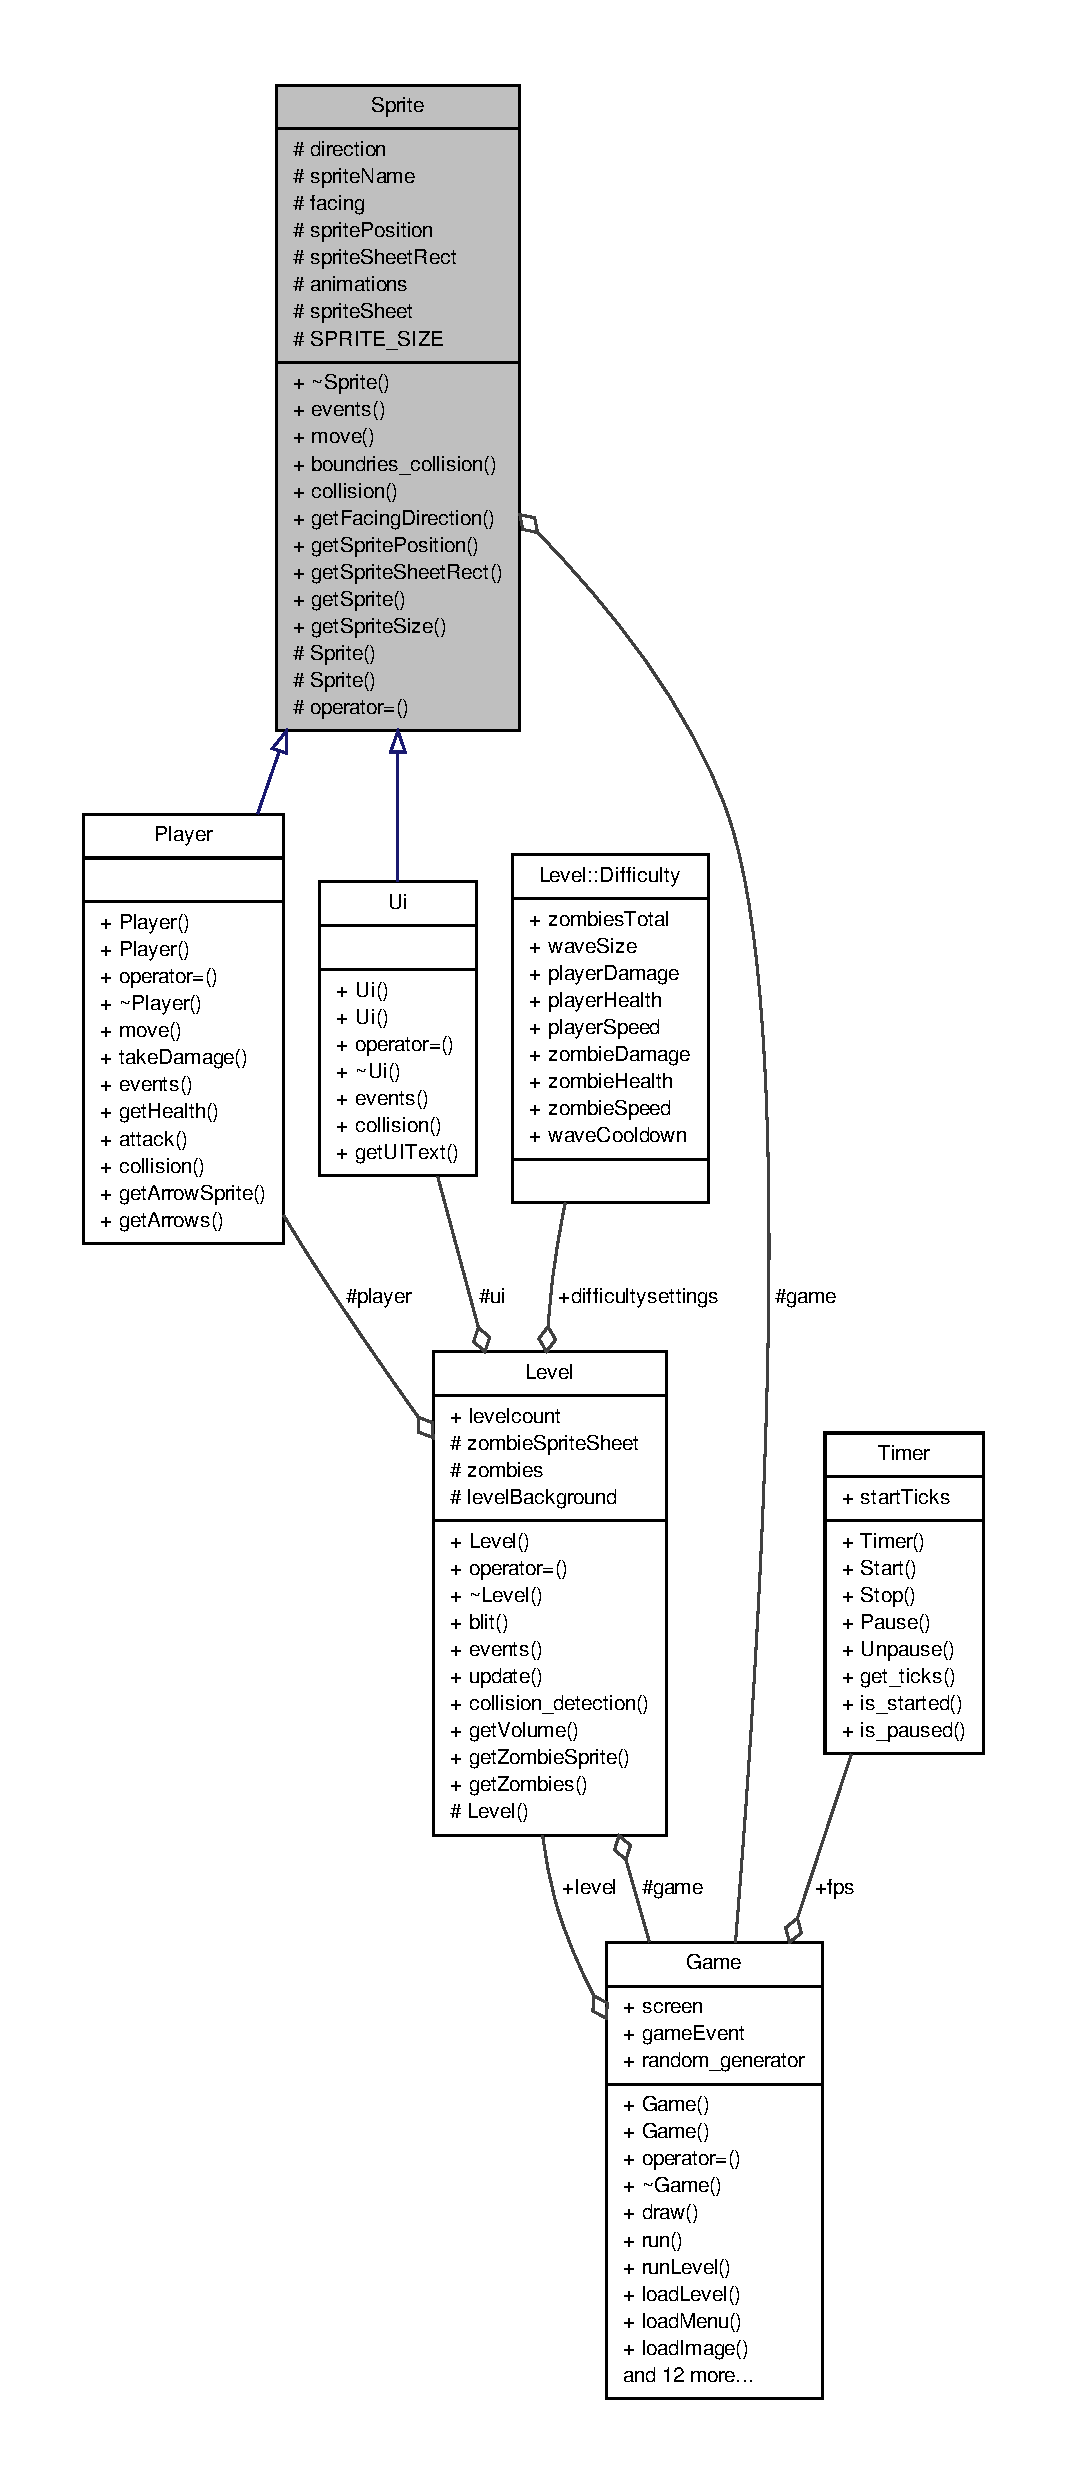
\includegraphics[height=550pt]{classSprite__coll__graph}
\end{center}
\end{figure}
\subsection*{Public Member Functions}
\begin{DoxyCompactItemize}
\item 
virtual \hyperlink{classSprite_a8accab430f9d90ae5117b57d67e32b84}{$\sim$\-Sprite} ()
\item 
virtual void \hyperlink{classSprite_a82cd02f494fe948457a8feb5ecd93212}{events} ()
\item 
virtual void \hyperlink{classSprite_afcf196c3d93fd743fdcc6f84d128ece6}{move} ()
\item 
virtual bool \hyperlink{classSprite_a82752d76482fb36ac5d3a22d86a50251}{boundries\-\_\-collision} ()
\item 
virtual bool \hyperlink{classSprite_ae0c21af6a4fc7fb8e9daf72675a1ec50}{collision} ()=0
\item 
std\-::string \hyperlink{classSprite_a5c3b19e7e0c8d831082c72a0b1aecd05}{get\-Facing\-Direction} () const 
\item 
S\-D\-L\-\_\-\-Rect \& \hyperlink{classSprite_a9009a87de777c6b9e0878b42716f159e}{get\-Sprite\-Position} ()
\item 
S\-D\-L\-\_\-\-Rect $\ast$ \hyperlink{classSprite_aa000074f1bd6ee67be85397d9b58e24d}{get\-Sprite\-Sheet\-Rect} ()
\item 
S\-D\-L\-\_\-\-Surface $\ast$ \hyperlink{classSprite_a8f1f384e8564dbd0ad18c75e782abb0f}{get\-Sprite} () const 
\item 
int \hyperlink{classSprite_abd54a55219e28b8865ee2ee177bc2811}{get\-Sprite\-Size} () const 
\end{DoxyCompactItemize}
\subsection*{Protected Member Functions}
\begin{DoxyCompactItemize}
\item 
\hyperlink{classSprite_a569ab75b5c75faa42c6ec2cfc14886ab}{Sprite} (\hyperlink{classGame}{Game} $\ast$\hyperlink{classSprite_a72c2faa2522184ea3cd81a1d50168a34}{game}, std\-::string name, S\-D\-L\-\_\-\-Surface $\ast$sprite\-Image=nullptr)
\item 
\hyperlink{classSprite_ab216809ce70a929c1e4407ce39b57547}{Sprite} (const \hyperlink{classSprite}{Sprite} \&)=delete
\item 
\hyperlink{classSprite}{Sprite} \& \hyperlink{classSprite_ab608eb8af8a6d50d3fd784170102cbc6}{operator=} (const \hyperlink{classSprite}{Sprite} \&)=delete
\end{DoxyCompactItemize}
\subsection*{Protected Attributes}
\begin{DoxyCompactItemize}
\item 
\hyperlink{classGame}{Game} $\ast$ \hyperlink{classSprite_a72c2faa2522184ea3cd81a1d50168a34}{game}
\item 
std\-::map$<$ std\-::string, int $>$ \hyperlink{classSprite_a660cef010618bdc48d706e0b3ab87177}{direction} \{\}
\item 
std\-::string \hyperlink{classSprite_a851a41894b0bbcb60a437fe82940fed9}{sprite\-Name} \{\}
\item 
std\-::string \hyperlink{classSprite_a582745bcb30f1910d056bf2ab5237e5b}{facing} \{\}
\item 
S\-D\-L\-\_\-\-Rect \hyperlink{classSprite_a2af2790211c2a3deb4a830741b0f8876}{sprite\-Position}
\item 
S\-D\-L\-\_\-\-Rect \hyperlink{classSprite_aac23050a3e3383f85f3cabbb874ff890}{sprite\-Sheet\-Rect}
\item 
\hyperlink{sprite_8h_a4e660753b3d87694743ccaf2bbc9150a}{animation\-Table} const \hyperlink{classSprite_aba52ded16f7623eb5f2ee63ece6ab896}{animations}
\item 
S\-D\-L\-\_\-\-Surface $\ast$ \hyperlink{classSprite_aa356e52e44c86d8d76cc3060eb41ae06}{sprite\-Sheet}
\item 
int \hyperlink{classSprite_a5dcf6606ddb6f6e8f85ad7d31536cc46}{S\-P\-R\-I\-T\-E\-\_\-\-S\-I\-Z\-E} \{0\}
\end{DoxyCompactItemize}


\subsection{Constructor \& Destructor Documentation}
\hypertarget{classSprite_a8accab430f9d90ae5117b57d67e32b84}{\index{Sprite@{Sprite}!$\sim$\-Sprite@{$\sim$\-Sprite}}
\index{$\sim$\-Sprite@{$\sim$\-Sprite}!Sprite@{Sprite}}
\subsubsection[{$\sim$\-Sprite}]{\setlength{\rightskip}{0pt plus 5cm}Sprite\-::$\sim$\-Sprite (
\begin{DoxyParamCaption}
{}
\end{DoxyParamCaption}
)\hspace{0.3cm}{\ttfamily [virtual]}}}\label{classSprite_a8accab430f9d90ae5117b57d67e32b84}
\hypertarget{classSprite_a569ab75b5c75faa42c6ec2cfc14886ab}{\index{Sprite@{Sprite}!Sprite@{Sprite}}
\index{Sprite@{Sprite}!Sprite@{Sprite}}
\subsubsection[{Sprite}]{\setlength{\rightskip}{0pt plus 5cm}Sprite\-::\-Sprite (
\begin{DoxyParamCaption}
\item[{{\bf Game} $\ast$}]{game, }
\item[{std\-::string}]{name, }
\item[{S\-D\-L\-\_\-\-Surface $\ast$}]{sprite\-Image = {\ttfamily nullptr}}
\end{DoxyParamCaption}
)\hspace{0.3cm}{\ttfamily [protected]}}}\label{classSprite_a569ab75b5c75faa42c6ec2cfc14886ab}
the sprite constructor sets all nessecary pointers internally, gets the sprite name creates a map holding the directions that a sprite can move, including its corresponding value that is later used to calculate and update sprite positions.\hypertarget{classSprite_ab216809ce70a929c1e4407ce39b57547}{\index{Sprite@{Sprite}!Sprite@{Sprite}}
\index{Sprite@{Sprite}!Sprite@{Sprite}}
\subsubsection[{Sprite}]{\setlength{\rightskip}{0pt plus 5cm}Sprite\-::\-Sprite (
\begin{DoxyParamCaption}
\item[{const {\bf Sprite} \&}]{}
\end{DoxyParamCaption}
)\hspace{0.3cm}{\ttfamily [protected]}, {\ttfamily [delete]}}}\label{classSprite_ab216809ce70a929c1e4407ce39b57547}


\subsection{Member Function Documentation}
\hypertarget{classSprite_a82752d76482fb36ac5d3a22d86a50251}{\index{Sprite@{Sprite}!boundries\-\_\-collision@{boundries\-\_\-collision}}
\index{boundries\-\_\-collision@{boundries\-\_\-collision}!Sprite@{Sprite}}
\subsubsection[{boundries\-\_\-collision}]{\setlength{\rightskip}{0pt plus 5cm}bool Sprite\-::boundries\-\_\-collision (
\begin{DoxyParamCaption}
{}
\end{DoxyParamCaption}
)\hspace{0.3cm}{\ttfamily [virtual]}}}\label{classSprite_a82752d76482fb36ac5d3a22d86a50251}
this is a virtual function handling the boundry collisions for all types of sprites.\hypertarget{classSprite_ae0c21af6a4fc7fb8e9daf72675a1ec50}{\index{Sprite@{Sprite}!collision@{collision}}
\index{collision@{collision}!Sprite@{Sprite}}
\subsubsection[{collision}]{\setlength{\rightskip}{0pt plus 5cm}virtual bool Sprite\-::collision (
\begin{DoxyParamCaption}
{}
\end{DoxyParamCaption}
)\hspace{0.3cm}{\ttfamily [pure virtual]}}}\label{classSprite_ae0c21af6a4fc7fb8e9daf72675a1ec50}


Implemented in \hyperlink{classZombie_a41b274a28ed94dddb23794e6f6cc81f1}{Zombie}, \hyperlink{classPlayer_a740c5163bb90b6b5824aed4817b0c2cc}{Player}, \hyperlink{classUi_ad1dd6e7fe4739c9a7f8c4d38e52b08ce}{Ui}, and \hyperlink{classArrow_aab2752bc7867eb7595a959189e0eb667}{Arrow}.

\hypertarget{classSprite_a82cd02f494fe948457a8feb5ecd93212}{\index{Sprite@{Sprite}!events@{events}}
\index{events@{events}!Sprite@{Sprite}}
\subsubsection[{events}]{\setlength{\rightskip}{0pt plus 5cm}void Sprite\-::events (
\begin{DoxyParamCaption}
{}
\end{DoxyParamCaption}
)\hspace{0.3cm}{\ttfamily [virtual]}}}\label{classSprite_a82cd02f494fe948457a8feb5ecd93212}


Reimplemented in \hyperlink{classZombie_af9f6fdd900c769f17d0e2dccb0db33c3}{Zombie}, \hyperlink{classPlayer_a9df270c5655b433d057e3e0f8fafd9ae}{Player}, and \hyperlink{classUi_ac9e709710a1c0f0ad61c3347026903fc}{Ui}.

\hypertarget{classSprite_a5c3b19e7e0c8d831082c72a0b1aecd05}{\index{Sprite@{Sprite}!get\-Facing\-Direction@{get\-Facing\-Direction}}
\index{get\-Facing\-Direction@{get\-Facing\-Direction}!Sprite@{Sprite}}
\subsubsection[{get\-Facing\-Direction}]{\setlength{\rightskip}{0pt plus 5cm}std\-::string Sprite\-::get\-Facing\-Direction (
\begin{DoxyParamCaption}
{}
\end{DoxyParamCaption}
) const}}\label{classSprite_a5c3b19e7e0c8d831082c72a0b1aecd05}
returns the direction a sprite is currently facing.\hypertarget{classSprite_a8f1f384e8564dbd0ad18c75e782abb0f}{\index{Sprite@{Sprite}!get\-Sprite@{get\-Sprite}}
\index{get\-Sprite@{get\-Sprite}!Sprite@{Sprite}}
\subsubsection[{get\-Sprite}]{\setlength{\rightskip}{0pt plus 5cm}S\-D\-L\-\_\-\-Surface $\ast$ Sprite\-::get\-Sprite (
\begin{DoxyParamCaption}
{}
\end{DoxyParamCaption}
) const}}\label{classSprite_a8f1f384e8564dbd0ad18c75e782abb0f}
returns the surface that holds the sprite.\hypertarget{classSprite_a9009a87de777c6b9e0878b42716f159e}{\index{Sprite@{Sprite}!get\-Sprite\-Position@{get\-Sprite\-Position}}
\index{get\-Sprite\-Position@{get\-Sprite\-Position}!Sprite@{Sprite}}
\subsubsection[{get\-Sprite\-Position}]{\setlength{\rightskip}{0pt plus 5cm}S\-D\-L\-\_\-\-Rect \& Sprite\-::get\-Sprite\-Position (
\begin{DoxyParamCaption}
{}
\end{DoxyParamCaption}
)}}\label{classSprite_a9009a87de777c6b9e0878b42716f159e}
returns a sprites current position on the level.\hypertarget{classSprite_aa000074f1bd6ee67be85397d9b58e24d}{\index{Sprite@{Sprite}!get\-Sprite\-Sheet\-Rect@{get\-Sprite\-Sheet\-Rect}}
\index{get\-Sprite\-Sheet\-Rect@{get\-Sprite\-Sheet\-Rect}!Sprite@{Sprite}}
\subsubsection[{get\-Sprite\-Sheet\-Rect}]{\setlength{\rightskip}{0pt plus 5cm}S\-D\-L\-\_\-\-Rect $\ast$ Sprite\-::get\-Sprite\-Sheet\-Rect (
\begin{DoxyParamCaption}
{}
\end{DoxyParamCaption}
)}}\label{classSprite_aa000074f1bd6ee67be85397d9b58e24d}
returns where in the sprite sheet the current animation is at.\hypertarget{classSprite_abd54a55219e28b8865ee2ee177bc2811}{\index{Sprite@{Sprite}!get\-Sprite\-Size@{get\-Sprite\-Size}}
\index{get\-Sprite\-Size@{get\-Sprite\-Size}!Sprite@{Sprite}}
\subsubsection[{get\-Sprite\-Size}]{\setlength{\rightskip}{0pt plus 5cm}int Sprite\-::get\-Sprite\-Size (
\begin{DoxyParamCaption}
{}
\end{DoxyParamCaption}
) const}}\label{classSprite_abd54a55219e28b8865ee2ee177bc2811}
returns the size of the sprite.\hypertarget{classSprite_afcf196c3d93fd743fdcc6f84d128ece6}{\index{Sprite@{Sprite}!move@{move}}
\index{move@{move}!Sprite@{Sprite}}
\subsubsection[{move}]{\setlength{\rightskip}{0pt plus 5cm}void Sprite\-::move (
\begin{DoxyParamCaption}
{}
\end{DoxyParamCaption}
)\hspace{0.3cm}{\ttfamily [virtual]}}}\label{classSprite_afcf196c3d93fd743fdcc6f84d128ece6}


Reimplemented in \hyperlink{classZombie_adc60ee88311d12f8fe150f5917943d2b}{Zombie}, \hyperlink{classPlayer_ae02ee46d8c20dd0697b975f935b09839}{Player}, and \hyperlink{classArrow_aab8bcf5d8e523c6d992c96af645dd30a}{Arrow}.

\hypertarget{classSprite_ab608eb8af8a6d50d3fd784170102cbc6}{\index{Sprite@{Sprite}!operator=@{operator=}}
\index{operator=@{operator=}!Sprite@{Sprite}}
\subsubsection[{operator=}]{\setlength{\rightskip}{0pt plus 5cm}{\bf Sprite}\& Sprite\-::operator= (
\begin{DoxyParamCaption}
\item[{const {\bf Sprite} \&}]{}
\end{DoxyParamCaption}
)\hspace{0.3cm}{\ttfamily [protected]}, {\ttfamily [delete]}}}\label{classSprite_ab608eb8af8a6d50d3fd784170102cbc6}


\subsection{Member Data Documentation}
\hypertarget{classSprite_aba52ded16f7623eb5f2ee63ece6ab896}{\index{Sprite@{Sprite}!animations@{animations}}
\index{animations@{animations}!Sprite@{Sprite}}
\subsubsection[{animations}]{\setlength{\rightskip}{0pt plus 5cm}{\bf animation\-Table} const Sprite\-::animations\hspace{0.3cm}{\ttfamily [protected]}}}\label{classSprite_aba52ded16f7623eb5f2ee63ece6ab896}
{\bfseries Initial value\-:}
\begin{DoxyCode}
=
        \{
                    \{\textcolor{stringliteral}{"upAnimation1"}, std::make\_pair(0, 0)\},
                    \{\textcolor{stringliteral}{"upAnimation2"}, std::make\_pair(25, 0)\},
                    \{\textcolor{stringliteral}{"rightAnimation1"}, std::make\_pair(50, 0)\},
                    \{\textcolor{stringliteral}{"rightAnimation2"}, std::make\_pair(75, 0)\},
                    \{\textcolor{stringliteral}{"downAnimation1"}, std::make\_pair(100, 0)\},
                    \{\textcolor{stringliteral}{"downAnimation2"}, std::make\_pair(125, 0)\},
                    \{\textcolor{stringliteral}{"leftAnimation1"}, std::make\_pair(150, 0)\},
                    \{\textcolor{stringliteral}{"leftAnimation2"}, std::make\_pair(175, 0)\},
                    \{\textcolor{stringliteral}{"upArrowAnimation"}, std::make\_pair(0, 0)\},
                    \{\textcolor{stringliteral}{"rightArrowAnimation"}, std::make\_pair(10, 0)\},
                    \{\textcolor{stringliteral}{"downArrowAnimation"}, std::make\_pair(20, 0)\},
                    \{\textcolor{stringliteral}{"leftArrowAnimation"}, std::make\_pair(30, 0)\},
                    \{\textcolor{stringliteral}{"lowHealthAnimation"}, std::make\_pair(0, 0)\},
                    \{\textcolor{stringliteral}{"mediumHealthAnimation"}, std::make\_pair(56, 0)\},
                    \{\textcolor{stringliteral}{"almostfullHealthAnimation"}, std::make\_pair(112, 0)\},
                    \{\textcolor{stringliteral}{"fullHealthAnimation"}, std::make\_pair(168, 0)\}
        \}
\end{DoxyCode}
\hypertarget{classSprite_a660cef010618bdc48d706e0b3ab87177}{\index{Sprite@{Sprite}!direction@{direction}}
\index{direction@{direction}!Sprite@{Sprite}}
\subsubsection[{direction}]{\setlength{\rightskip}{0pt plus 5cm}std\-::map$<$std\-::string, int$>$ Sprite\-::direction \{\}\hspace{0.3cm}{\ttfamily [protected]}}}\label{classSprite_a660cef010618bdc48d706e0b3ab87177}
\hypertarget{classSprite_a582745bcb30f1910d056bf2ab5237e5b}{\index{Sprite@{Sprite}!facing@{facing}}
\index{facing@{facing}!Sprite@{Sprite}}
\subsubsection[{facing}]{\setlength{\rightskip}{0pt plus 5cm}std\-::string Sprite\-::facing \{\}\hspace{0.3cm}{\ttfamily [protected]}}}\label{classSprite_a582745bcb30f1910d056bf2ab5237e5b}
\hypertarget{classSprite_a72c2faa2522184ea3cd81a1d50168a34}{\index{Sprite@{Sprite}!game@{game}}
\index{game@{game}!Sprite@{Sprite}}
\subsubsection[{game}]{\setlength{\rightskip}{0pt plus 5cm}{\bf Game}$\ast$ Sprite\-::game\hspace{0.3cm}{\ttfamily [protected]}}}\label{classSprite_a72c2faa2522184ea3cd81a1d50168a34}
\hypertarget{classSprite_a5dcf6606ddb6f6e8f85ad7d31536cc46}{\index{Sprite@{Sprite}!S\-P\-R\-I\-T\-E\-\_\-\-S\-I\-Z\-E@{S\-P\-R\-I\-T\-E\-\_\-\-S\-I\-Z\-E}}
\index{S\-P\-R\-I\-T\-E\-\_\-\-S\-I\-Z\-E@{S\-P\-R\-I\-T\-E\-\_\-\-S\-I\-Z\-E}!Sprite@{Sprite}}
\subsubsection[{S\-P\-R\-I\-T\-E\-\_\-\-S\-I\-Z\-E}]{\setlength{\rightskip}{0pt plus 5cm}int Sprite\-::\-S\-P\-R\-I\-T\-E\-\_\-\-S\-I\-Z\-E \{0\}\hspace{0.3cm}{\ttfamily [protected]}}}\label{classSprite_a5dcf6606ddb6f6e8f85ad7d31536cc46}
\hypertarget{classSprite_a851a41894b0bbcb60a437fe82940fed9}{\index{Sprite@{Sprite}!sprite\-Name@{sprite\-Name}}
\index{sprite\-Name@{sprite\-Name}!Sprite@{Sprite}}
\subsubsection[{sprite\-Name}]{\setlength{\rightskip}{0pt plus 5cm}std\-::string Sprite\-::sprite\-Name \{\}\hspace{0.3cm}{\ttfamily [protected]}}}\label{classSprite_a851a41894b0bbcb60a437fe82940fed9}
\hypertarget{classSprite_a2af2790211c2a3deb4a830741b0f8876}{\index{Sprite@{Sprite}!sprite\-Position@{sprite\-Position}}
\index{sprite\-Position@{sprite\-Position}!Sprite@{Sprite}}
\subsubsection[{sprite\-Position}]{\setlength{\rightskip}{0pt plus 5cm}S\-D\-L\-\_\-\-Rect Sprite\-::sprite\-Position\hspace{0.3cm}{\ttfamily [protected]}}}\label{classSprite_a2af2790211c2a3deb4a830741b0f8876}
\hypertarget{classSprite_aa356e52e44c86d8d76cc3060eb41ae06}{\index{Sprite@{Sprite}!sprite\-Sheet@{sprite\-Sheet}}
\index{sprite\-Sheet@{sprite\-Sheet}!Sprite@{Sprite}}
\subsubsection[{sprite\-Sheet}]{\setlength{\rightskip}{0pt plus 5cm}S\-D\-L\-\_\-\-Surface$\ast$ Sprite\-::sprite\-Sheet\hspace{0.3cm}{\ttfamily [protected]}}}\label{classSprite_aa356e52e44c86d8d76cc3060eb41ae06}
\hypertarget{classSprite_aac23050a3e3383f85f3cabbb874ff890}{\index{Sprite@{Sprite}!sprite\-Sheet\-Rect@{sprite\-Sheet\-Rect}}
\index{sprite\-Sheet\-Rect@{sprite\-Sheet\-Rect}!Sprite@{Sprite}}
\subsubsection[{sprite\-Sheet\-Rect}]{\setlength{\rightskip}{0pt plus 5cm}S\-D\-L\-\_\-\-Rect Sprite\-::sprite\-Sheet\-Rect\hspace{0.3cm}{\ttfamily [protected]}}}\label{classSprite_aac23050a3e3383f85f3cabbb874ff890}


The documentation for this class was generated from the following files\-:\begin{DoxyCompactItemize}
\item 
\hyperlink{sprite_8h}{sprite.\-h}\item 
\hyperlink{sprite_8cc}{sprite.\-cc}\end{DoxyCompactItemize}

\hypertarget{classTimer}{\section{Timer Class Reference}
\label{classTimer}\index{Timer@{Timer}}
}


{\ttfamily \#include $<$timer.\-h$>$}



Collaboration diagram for Timer\-:\nopagebreak
\begin{figure}[H]
\begin{center}
\leavevmode
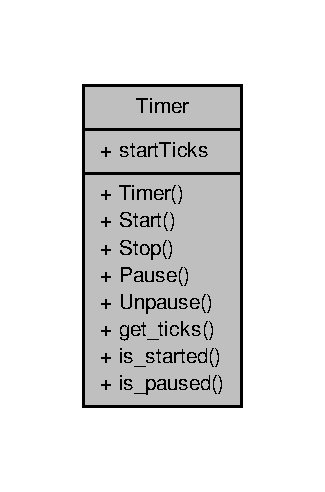
\includegraphics[width=156pt]{classTimer__coll__graph}
\end{center}
\end{figure}
\subsection*{Public Member Functions}
\begin{DoxyCompactItemize}
\item 
\hyperlink{classTimer_a5f16e8da27d2a5a5242dead46de05d97}{Timer} ()
\item 
void \hyperlink{classTimer_a4e607b129b392c11adddd9641a320436}{Start} ()
\item 
void \hyperlink{classTimer_a6379e797f968aaee6ac3bb12dc6b81c5}{Stop} ()
\item 
void \hyperlink{classTimer_a9b8c57bf9675da635a82d68d9b4d05e5}{Pause} ()
\item 
void \hyperlink{classTimer_a18bae6d4516c122edd3489b7dccefa70}{Unpause} ()
\item 
int \hyperlink{classTimer_a56d411d072f1cc22b53f6ccb74cc7f63}{get\-\_\-ticks} ()
\item 
bool \hyperlink{classTimer_a8aabbd05a0fc030e7156b01bcd8264db}{is\-\_\-started} ()
\item 
bool \hyperlink{classTimer_a18c977688b4e0809cb603e9abb265950}{is\-\_\-paused} ()
\end{DoxyCompactItemize}
\subsection*{Public Attributes}
\begin{DoxyCompactItemize}
\item 
int \hyperlink{classTimer_ad6e980d932698bb8fd82498e6c47696c}{start\-Ticks} \{0\}
\end{DoxyCompactItemize}


\subsection{Constructor \& Destructor Documentation}
\hypertarget{classTimer_a5f16e8da27d2a5a5242dead46de05d97}{\index{Timer@{Timer}!Timer@{Timer}}
\index{Timer@{Timer}!Timer@{Timer}}
\subsubsection[{Timer}]{\setlength{\rightskip}{0pt plus 5cm}Timer\-::\-Timer (
\begin{DoxyParamCaption}
{}
\end{DoxyParamCaption}
)}}\label{classTimer_a5f16e8da27d2a5a5242dead46de05d97}


\subsection{Member Function Documentation}
\hypertarget{classTimer_a56d411d072f1cc22b53f6ccb74cc7f63}{\index{Timer@{Timer}!get\-\_\-ticks@{get\-\_\-ticks}}
\index{get\-\_\-ticks@{get\-\_\-ticks}!Timer@{Timer}}
\subsubsection[{get\-\_\-ticks}]{\setlength{\rightskip}{0pt plus 5cm}int Timer\-::get\-\_\-ticks (
\begin{DoxyParamCaption}
{}
\end{DoxyParamCaption}
)}}\label{classTimer_a56d411d072f1cc22b53f6ccb74cc7f63}
\hypertarget{classTimer_a18c977688b4e0809cb603e9abb265950}{\index{Timer@{Timer}!is\-\_\-paused@{is\-\_\-paused}}
\index{is\-\_\-paused@{is\-\_\-paused}!Timer@{Timer}}
\subsubsection[{is\-\_\-paused}]{\setlength{\rightskip}{0pt plus 5cm}bool Timer\-::is\-\_\-paused (
\begin{DoxyParamCaption}
{}
\end{DoxyParamCaption}
)}}\label{classTimer_a18c977688b4e0809cb603e9abb265950}
\hypertarget{classTimer_a8aabbd05a0fc030e7156b01bcd8264db}{\index{Timer@{Timer}!is\-\_\-started@{is\-\_\-started}}
\index{is\-\_\-started@{is\-\_\-started}!Timer@{Timer}}
\subsubsection[{is\-\_\-started}]{\setlength{\rightskip}{0pt plus 5cm}bool Timer\-::is\-\_\-started (
\begin{DoxyParamCaption}
{}
\end{DoxyParamCaption}
)}}\label{classTimer_a8aabbd05a0fc030e7156b01bcd8264db}
\hypertarget{classTimer_a9b8c57bf9675da635a82d68d9b4d05e5}{\index{Timer@{Timer}!Pause@{Pause}}
\index{Pause@{Pause}!Timer@{Timer}}
\subsubsection[{Pause}]{\setlength{\rightskip}{0pt plus 5cm}void Timer\-::\-Pause (
\begin{DoxyParamCaption}
{}
\end{DoxyParamCaption}
)}}\label{classTimer_a9b8c57bf9675da635a82d68d9b4d05e5}
\hypertarget{classTimer_a4e607b129b392c11adddd9641a320436}{\index{Timer@{Timer}!Start@{Start}}
\index{Start@{Start}!Timer@{Timer}}
\subsubsection[{Start}]{\setlength{\rightskip}{0pt plus 5cm}void Timer\-::\-Start (
\begin{DoxyParamCaption}
{}
\end{DoxyParamCaption}
)}}\label{classTimer_a4e607b129b392c11adddd9641a320436}
\hypertarget{classTimer_a6379e797f968aaee6ac3bb12dc6b81c5}{\index{Timer@{Timer}!Stop@{Stop}}
\index{Stop@{Stop}!Timer@{Timer}}
\subsubsection[{Stop}]{\setlength{\rightskip}{0pt plus 5cm}void Timer\-::\-Stop (
\begin{DoxyParamCaption}
{}
\end{DoxyParamCaption}
)}}\label{classTimer_a6379e797f968aaee6ac3bb12dc6b81c5}
\hypertarget{classTimer_a18bae6d4516c122edd3489b7dccefa70}{\index{Timer@{Timer}!Unpause@{Unpause}}
\index{Unpause@{Unpause}!Timer@{Timer}}
\subsubsection[{Unpause}]{\setlength{\rightskip}{0pt plus 5cm}void Timer\-::\-Unpause (
\begin{DoxyParamCaption}
{}
\end{DoxyParamCaption}
)}}\label{classTimer_a18bae6d4516c122edd3489b7dccefa70}


\subsection{Member Data Documentation}
\hypertarget{classTimer_ad6e980d932698bb8fd82498e6c47696c}{\index{Timer@{Timer}!start\-Ticks@{start\-Ticks}}
\index{start\-Ticks@{start\-Ticks}!Timer@{Timer}}
\subsubsection[{start\-Ticks}]{\setlength{\rightskip}{0pt plus 5cm}int Timer\-::start\-Ticks \{0\}}}\label{classTimer_ad6e980d932698bb8fd82498e6c47696c}


The documentation for this class was generated from the following files\-:\begin{DoxyCompactItemize}
\item 
\hyperlink{timer_8h}{timer.\-h}\item 
\hyperlink{timer_8cc}{timer.\-cc}\end{DoxyCompactItemize}

\hypertarget{classUi}{\section{Ui Class Reference}
\label{classUi}\index{Ui@{Ui}}
}


{\ttfamily \#include $<$U\-I.\-h$>$}



Inheritance diagram for Ui\-:\nopagebreak
\begin{figure}[H]
\begin{center}
\leavevmode
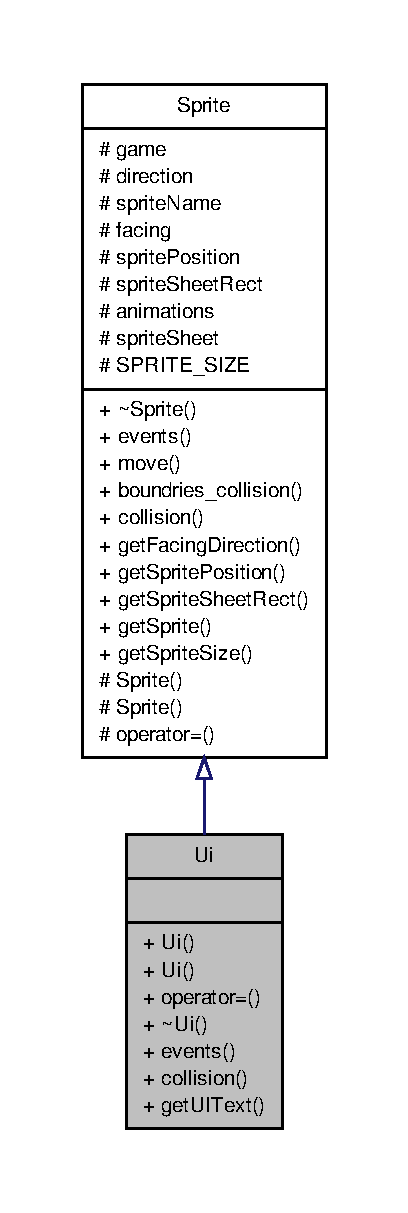
\includegraphics[height=550pt]{classUi__inherit__graph}
\end{center}
\end{figure}


Collaboration diagram for Ui\-:
\nopagebreak
\begin{figure}[H]
\begin{center}
\leavevmode
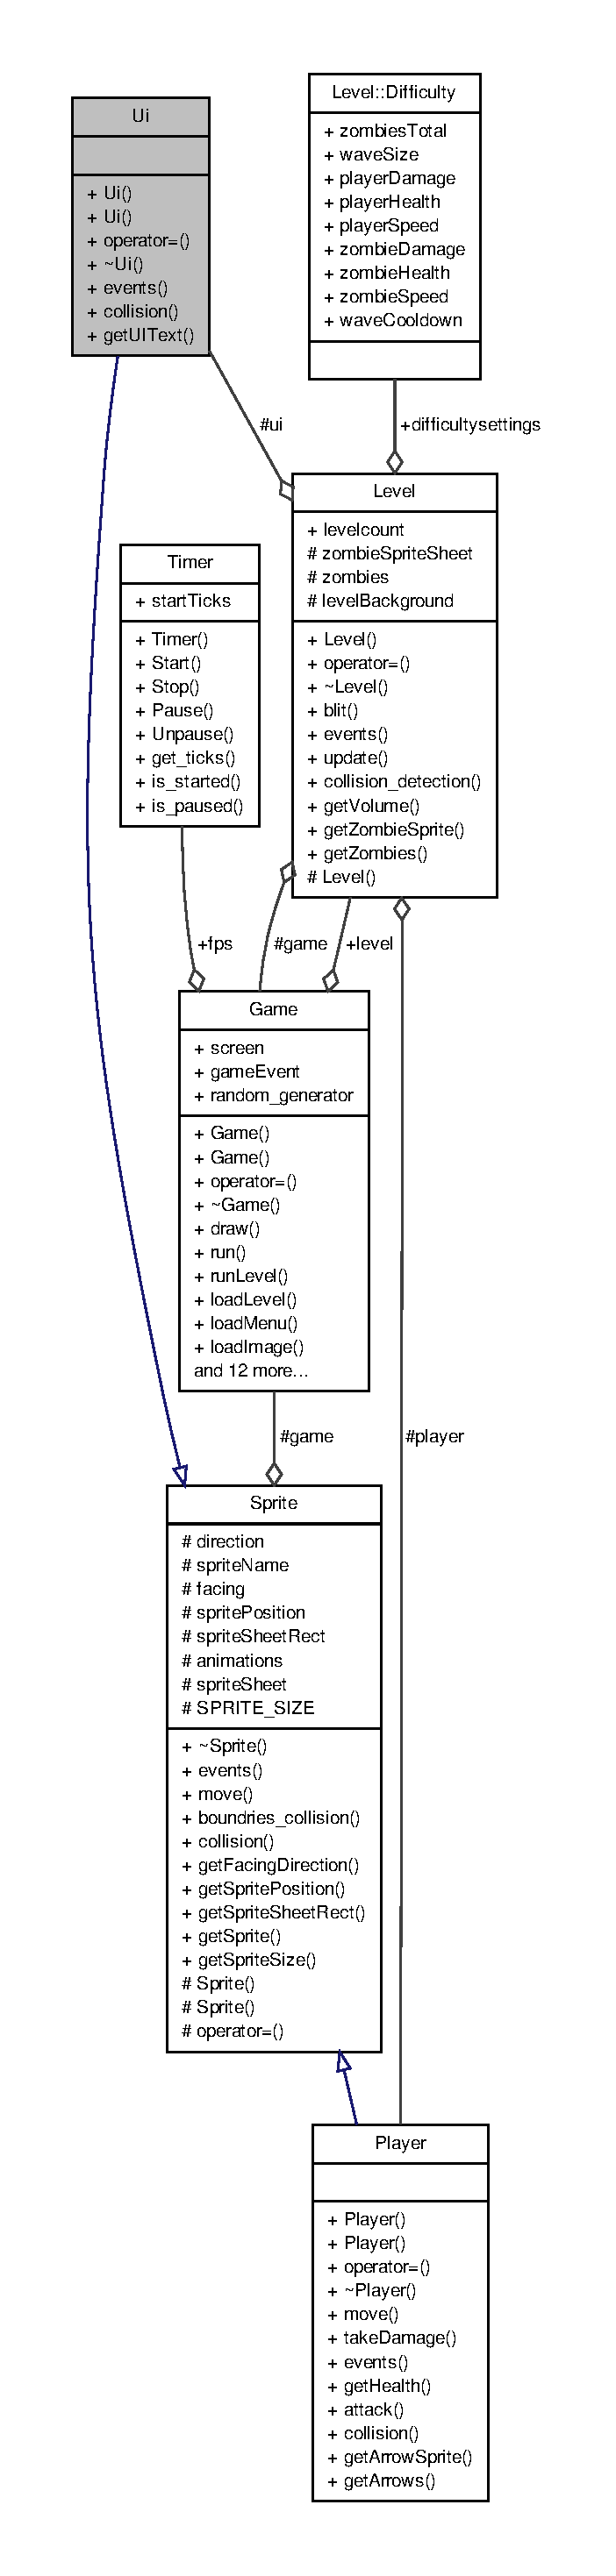
\includegraphics[height=550pt]{classUi__coll__graph}
\end{center}
\end{figure}
\subsection*{Public Member Functions}
\begin{DoxyCompactItemize}
\item 
\hyperlink{classUi_a55c1d53a31ec024b82ce901a3ea2e4d9}{Ui} (\hyperlink{classGame}{Game} $\ast$game, \hyperlink{classPlayer}{Player} $\ast$player)
\item 
\hyperlink{classUi_aa6c7ed33d913ad19c82b6bb7e010a92f}{Ui} (const \hyperlink{classUi}{Ui} \&)=delete
\item 
\hyperlink{classUi}{Ui} \& \hyperlink{classUi_a7adc143e966ada55593ebd0607e8255d}{operator=} (const \hyperlink{classUi}{Ui} \&)=delete
\item 
\hyperlink{classUi_a7a0333fdf87c857f3b780015ee8e3bd9}{$\sim$\-Ui} ()
\item 
void \hyperlink{classUi_ac9e709710a1c0f0ad61c3347026903fc}{events} ()
\item 
bool \hyperlink{classUi_ad1dd6e7fe4739c9a7f8c4d38e52b08ce}{collision} ()
\item 
S\-D\-L\-\_\-\-Surface $\ast$ \hyperlink{classUi_a89b63a847637f8ec9d6148d7367d5857}{get\-U\-I\-Text} () const 
\end{DoxyCompactItemize}
\subsection*{Additional Inherited Members}


\subsection{Constructor \& Destructor Documentation}
\hypertarget{classUi_a55c1d53a31ec024b82ce901a3ea2e4d9}{\index{Ui@{Ui}!Ui@{Ui}}
\index{Ui@{Ui}!Ui@{Ui}}
\subsubsection[{Ui}]{\setlength{\rightskip}{0pt plus 5cm}Ui\-::\-Ui (
\begin{DoxyParamCaption}
\item[{{\bf Game} $\ast$}]{game, }
\item[{{\bf Player} $\ast$}]{player}
\end{DoxyParamCaption}
)}}\label{classUi_a55c1d53a31ec024b82ce901a3ea2e4d9}
the user interface draws the players health bar, the text on screen, it also opens the true type font system.\hypertarget{classUi_aa6c7ed33d913ad19c82b6bb7e010a92f}{\index{Ui@{Ui}!Ui@{Ui}}
\index{Ui@{Ui}!Ui@{Ui}}
\subsubsection[{Ui}]{\setlength{\rightskip}{0pt plus 5cm}Ui\-::\-Ui (
\begin{DoxyParamCaption}
\item[{const {\bf Ui} \&}]{}
\end{DoxyParamCaption}
)\hspace{0.3cm}{\ttfamily [delete]}}}\label{classUi_aa6c7ed33d913ad19c82b6bb7e010a92f}
\hypertarget{classUi_a7a0333fdf87c857f3b780015ee8e3bd9}{\index{Ui@{Ui}!$\sim$\-Ui@{$\sim$\-Ui}}
\index{$\sim$\-Ui@{$\sim$\-Ui}!Ui@{Ui}}
\subsubsection[{$\sim$\-Ui}]{\setlength{\rightskip}{0pt plus 5cm}Ui\-::$\sim$\-Ui (
\begin{DoxyParamCaption}
{}
\end{DoxyParamCaption}
)}}\label{classUi_a7a0333fdf87c857f3b780015ee8e3bd9}
the destructor is resposible for freeing the surfaces and closing the true type font system.

\subsection{Member Function Documentation}
\hypertarget{classUi_ad1dd6e7fe4739c9a7f8c4d38e52b08ce}{\index{Ui@{Ui}!collision@{collision}}
\index{collision@{collision}!Ui@{Ui}}
\subsubsection[{collision}]{\setlength{\rightskip}{0pt plus 5cm}bool Ui\-::collision (
\begin{DoxyParamCaption}
{}
\end{DoxyParamCaption}
)\hspace{0.3cm}{\ttfamily [virtual]}}}\label{classUi_ad1dd6e7fe4739c9a7f8c4d38e52b08ce}


Implements \hyperlink{classSprite_ae0c21af6a4fc7fb8e9daf72675a1ec50}{Sprite}.

\hypertarget{classUi_ac9e709710a1c0f0ad61c3347026903fc}{\index{Ui@{Ui}!events@{events}}
\index{events@{events}!Ui@{Ui}}
\subsubsection[{events}]{\setlength{\rightskip}{0pt plus 5cm}void Ui\-::events (
\begin{DoxyParamCaption}
{}
\end{DoxyParamCaption}
)\hspace{0.3cm}{\ttfamily [virtual]}}}\label{classUi_ac9e709710a1c0f0ad61c3347026903fc}
we have to call on the user interface event function to update the player health bar.

Reimplemented from \hyperlink{classSprite_a82cd02f494fe948457a8feb5ecd93212}{Sprite}.

\hypertarget{classUi_a89b63a847637f8ec9d6148d7367d5857}{\index{Ui@{Ui}!get\-U\-I\-Text@{get\-U\-I\-Text}}
\index{get\-U\-I\-Text@{get\-U\-I\-Text}!Ui@{Ui}}
\subsubsection[{get\-U\-I\-Text}]{\setlength{\rightskip}{0pt plus 5cm}S\-D\-L\-\_\-\-Surface $\ast$ Ui\-::get\-U\-I\-Text (
\begin{DoxyParamCaption}
{}
\end{DoxyParamCaption}
) const}}\label{classUi_a89b63a847637f8ec9d6148d7367d5857}
returns the surface that holds the player health text message.\hypertarget{classUi_a7adc143e966ada55593ebd0607e8255d}{\index{Ui@{Ui}!operator=@{operator=}}
\index{operator=@{operator=}!Ui@{Ui}}
\subsubsection[{operator=}]{\setlength{\rightskip}{0pt plus 5cm}{\bf Ui}\& Ui\-::operator= (
\begin{DoxyParamCaption}
\item[{const {\bf Ui} \&}]{}
\end{DoxyParamCaption}
)\hspace{0.3cm}{\ttfamily [delete]}}}\label{classUi_a7adc143e966ada55593ebd0607e8255d}


The documentation for this class was generated from the following files\-:\begin{DoxyCompactItemize}
\item 
\hyperlink{UI_8h}{U\-I.\-h}\item 
\hyperlink{UI_8cc}{U\-I.\-cc}\item 
\hyperlink{UI_8cpp}{U\-I.\-cpp}\end{DoxyCompactItemize}

\hypertarget{classZombie}{\section{Zombie Class Reference}
\label{classZombie}\index{Zombie@{Zombie}}
}


{\ttfamily \#include $<$zombie.\-h$>$}



Inheritance diagram for Zombie\-:\nopagebreak
\begin{figure}[H]
\begin{center}
\leavevmode
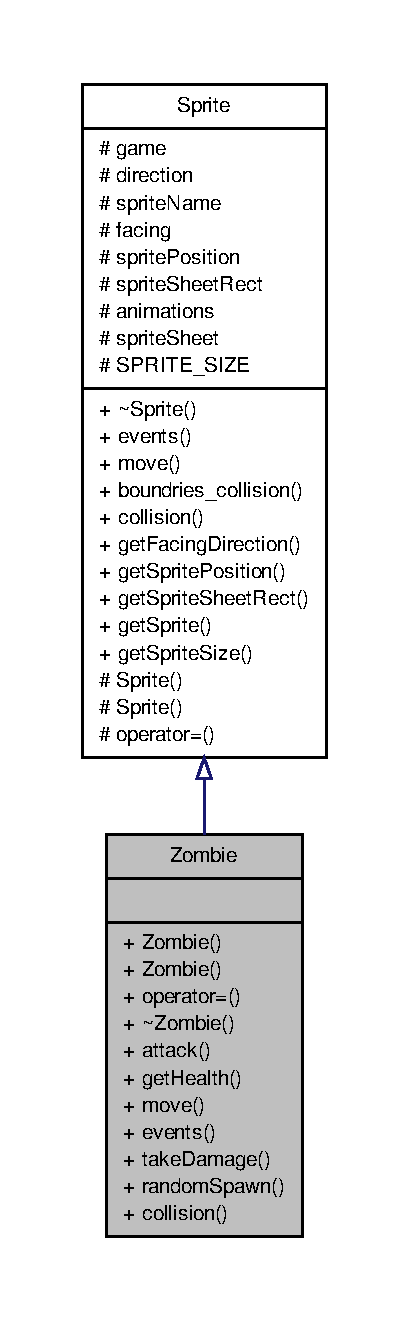
\includegraphics[height=550pt]{classZombie__inherit__graph}
\end{center}
\end{figure}


Collaboration diagram for Zombie\-:
\nopagebreak
\begin{figure}[H]
\begin{center}
\leavevmode
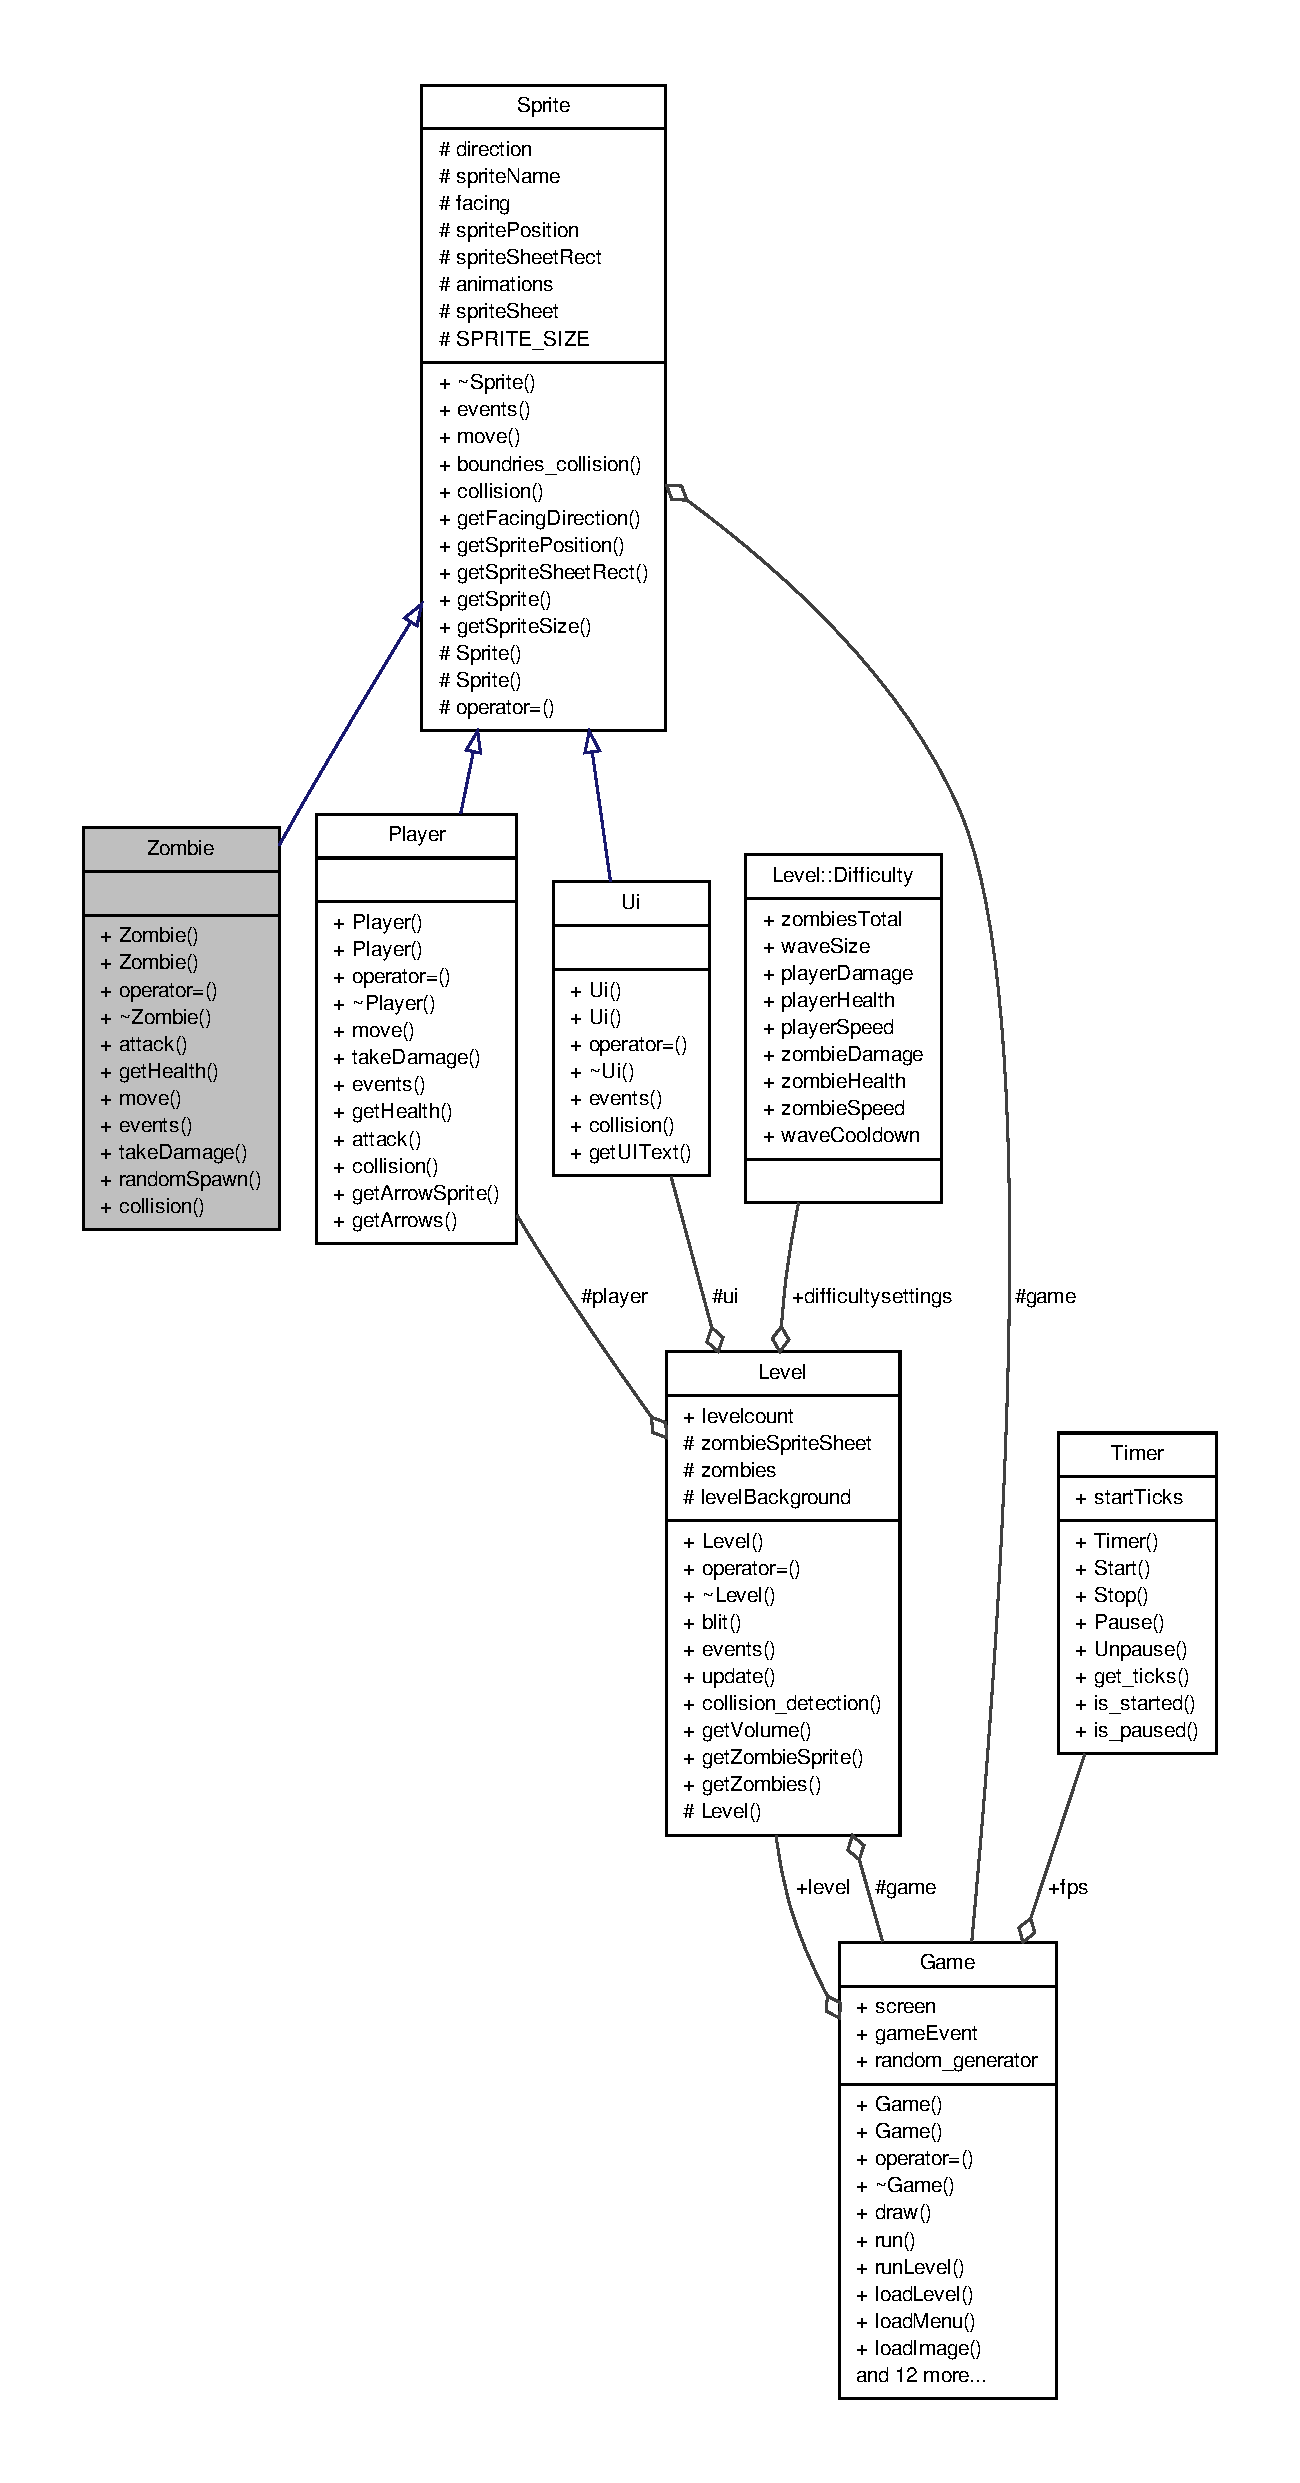
\includegraphics[height=550pt]{classZombie__coll__graph}
\end{center}
\end{figure}
\subsection*{Public Member Functions}
\begin{DoxyCompactItemize}
\item 
\hyperlink{classZombie_a490b91b7f34c4e3d8a3d4b42e6ef018c}{Zombie} (\hyperlink{classGame}{Game} $\ast$game\-Pointer, \hyperlink{classLevel}{Level} $\ast$level, std\-::string zombiename, \hyperlink{classPlayer}{Player} $\ast$player)
\item 
\hyperlink{classZombie_a1551812e760c7623f3b015e948d3d711}{Zombie} (const \hyperlink{classZombie}{Zombie} \&)=delete
\item 
\hyperlink{classZombie}{Zombie} \& \hyperlink{classZombie_ac110303450e69fd7cf672ac6812cbffe}{operator=} (const \hyperlink{classZombie}{Zombie} \&)=delete
\item 
\hyperlink{classZombie_ae3405ba8c88578dfa9d05cdeae0bab9f}{$\sim$\-Zombie} ()=default
\item 
int \hyperlink{classZombie_a7043da61be95308e7a952adaae347b7e}{attack} ()
\item 
int \hyperlink{classZombie_a2cf90eec8daea5e1cda6e3cdff4b0147}{get\-Health} () const 
\item 
void \hyperlink{classZombie_adc60ee88311d12f8fe150f5917943d2b}{move} ()
\item 
void \hyperlink{classZombie_af9f6fdd900c769f17d0e2dccb0db33c3}{events} ()
\item 
void \hyperlink{classZombie_a2fde39f3efac6da9062cf29e20c71b84}{take\-Damage} (int damage)
\item 
void \hyperlink{classZombie_ad45b25d75c9a2875a6b7fb8a272d2191}{random\-Spawn} ()
\item 
bool \hyperlink{classZombie_a41b274a28ed94dddb23794e6f6cc81f1}{collision} ()
\end{DoxyCompactItemize}
\subsection*{Additional Inherited Members}


\subsection{Constructor \& Destructor Documentation}
\hypertarget{classZombie_a490b91b7f34c4e3d8a3d4b42e6ef018c}{\index{Zombie@{Zombie}!Zombie@{Zombie}}
\index{Zombie@{Zombie}!Zombie@{Zombie}}
\subsubsection[{Zombie}]{\setlength{\rightskip}{0pt plus 5cm}Zombie\-::\-Zombie (
\begin{DoxyParamCaption}
\item[{{\bf Game} $\ast$}]{game\-Pointer, }
\item[{{\bf Level} $\ast$}]{level, }
\item[{std\-::string}]{zombiename, }
\item[{{\bf Player} $\ast$}]{player}
\end{DoxyParamCaption}
)}}\label{classZombie_a490b91b7f34c4e3d8a3d4b42e6ef018c}
the zombie constructor defaults the facing direction to down, sets the zombies health, damage and speed depending on which difficulty setting we are playing on. The constructor also randomizes the spawn location for the zombies and sets the initial animation frame in the sprite sheet.\hypertarget{classZombie_a1551812e760c7623f3b015e948d3d711}{\index{Zombie@{Zombie}!Zombie@{Zombie}}
\index{Zombie@{Zombie}!Zombie@{Zombie}}
\subsubsection[{Zombie}]{\setlength{\rightskip}{0pt plus 5cm}Zombie\-::\-Zombie (
\begin{DoxyParamCaption}
\item[{const {\bf Zombie} \&}]{}
\end{DoxyParamCaption}
)\hspace{0.3cm}{\ttfamily [delete]}}}\label{classZombie_a1551812e760c7623f3b015e948d3d711}
\hypertarget{classZombie_ae3405ba8c88578dfa9d05cdeae0bab9f}{\index{Zombie@{Zombie}!$\sim$\-Zombie@{$\sim$\-Zombie}}
\index{$\sim$\-Zombie@{$\sim$\-Zombie}!Zombie@{Zombie}}
\subsubsection[{$\sim$\-Zombie}]{\setlength{\rightskip}{0pt plus 5cm}Zombie\-::$\sim$\-Zombie (
\begin{DoxyParamCaption}
{}
\end{DoxyParamCaption}
)\hspace{0.3cm}{\ttfamily [default]}}}\label{classZombie_ae3405ba8c88578dfa9d05cdeae0bab9f}


\subsection{Member Function Documentation}
\hypertarget{classZombie_a7043da61be95308e7a952adaae347b7e}{\index{Zombie@{Zombie}!attack@{attack}}
\index{attack@{attack}!Zombie@{Zombie}}
\subsubsection[{attack}]{\setlength{\rightskip}{0pt plus 5cm}int Zombie\-::attack (
\begin{DoxyParamCaption}
{}
\end{DoxyParamCaption}
)}}\label{classZombie_a7043da61be95308e7a952adaae347b7e}
when the zombies collide with the player, we take damage equal to the zombies damage.\hypertarget{classZombie_a41b274a28ed94dddb23794e6f6cc81f1}{\index{Zombie@{Zombie}!collision@{collision}}
\index{collision@{collision}!Zombie@{Zombie}}
\subsubsection[{collision}]{\setlength{\rightskip}{0pt plus 5cm}bool Zombie\-::collision (
\begin{DoxyParamCaption}
{}
\end{DoxyParamCaption}
)\hspace{0.3cm}{\ttfamily [virtual]}}}\label{classZombie_a41b274a28ed94dddb23794e6f6cc81f1}
We check every zombie if they collide with each other 

Implements \hyperlink{classSprite_ae0c21af6a4fc7fb8e9daf72675a1ec50}{Sprite}.

\hypertarget{classZombie_af9f6fdd900c769f17d0e2dccb0db33c3}{\index{Zombie@{Zombie}!events@{events}}
\index{events@{events}!Zombie@{Zombie}}
\subsubsection[{events}]{\setlength{\rightskip}{0pt plus 5cm}void Zombie\-::events (
\begin{DoxyParamCaption}
{}
\end{DoxyParamCaption}
)\hspace{0.3cm}{\ttfamily [virtual]}}}\label{classZombie_af9f6fdd900c769f17d0e2dccb0db33c3}
the zombie has its own system of movement but uses the same system for facing, and animations

Reimplemented from \hyperlink{classSprite_a82cd02f494fe948457a8feb5ecd93212}{Sprite}.

\hypertarget{classZombie_a2cf90eec8daea5e1cda6e3cdff4b0147}{\index{Zombie@{Zombie}!get\-Health@{get\-Health}}
\index{get\-Health@{get\-Health}!Zombie@{Zombie}}
\subsubsection[{get\-Health}]{\setlength{\rightskip}{0pt plus 5cm}int Zombie\-::get\-Health (
\begin{DoxyParamCaption}
{}
\end{DoxyParamCaption}
) const}}\label{classZombie_a2cf90eec8daea5e1cda6e3cdff4b0147}
return the health of a zombie.\hypertarget{classZombie_adc60ee88311d12f8fe150f5917943d2b}{\index{Zombie@{Zombie}!move@{move}}
\index{move@{move}!Zombie@{Zombie}}
\subsubsection[{move}]{\setlength{\rightskip}{0pt plus 5cm}void Zombie\-::move (
\begin{DoxyParamCaption}
{}
\end{DoxyParamCaption}
)\hspace{0.3cm}{\ttfamily [virtual]}}}\label{classZombie_adc60ee88311d12f8fe150f5917943d2b}
the move function is based on the players movement so we can get some sense of artificial intelligence. However this function just finds the player in the x-\/axis and then walks towards the player in the y-\/axis, creating the effect of the zombies walking toward the player.

Reimplemented from \hyperlink{classSprite_afcf196c3d93fd743fdcc6f84d128ece6}{Sprite}.

\hypertarget{classZombie_ac110303450e69fd7cf672ac6812cbffe}{\index{Zombie@{Zombie}!operator=@{operator=}}
\index{operator=@{operator=}!Zombie@{Zombie}}
\subsubsection[{operator=}]{\setlength{\rightskip}{0pt plus 5cm}{\bf Zombie}\& Zombie\-::operator= (
\begin{DoxyParamCaption}
\item[{const {\bf Zombie} \&}]{}
\end{DoxyParamCaption}
)\hspace{0.3cm}{\ttfamily [delete]}}}\label{classZombie_ac110303450e69fd7cf672ac6812cbffe}
\hypertarget{classZombie_ad45b25d75c9a2875a6b7fb8a272d2191}{\index{Zombie@{Zombie}!random\-Spawn@{random\-Spawn}}
\index{random\-Spawn@{random\-Spawn}!Zombie@{Zombie}}
\subsubsection[{random\-Spawn}]{\setlength{\rightskip}{0pt plus 5cm}void Zombie\-::random\-Spawn (
\begin{DoxyParamCaption}
{}
\end{DoxyParamCaption}
)}}\label{classZombie_ad45b25d75c9a2875a6b7fb8a272d2191}
we have 4 different openings in the level that we can use to randomly select where we want to spawn the zombies. we use a random generator to choose a number between 1-\/4 , that number corresponds to coordinates on the level.\hypertarget{classZombie_a2fde39f3efac6da9062cf29e20c71b84}{\index{Zombie@{Zombie}!take\-Damage@{take\-Damage}}
\index{take\-Damage@{take\-Damage}!Zombie@{Zombie}}
\subsubsection[{take\-Damage}]{\setlength{\rightskip}{0pt plus 5cm}void Zombie\-::take\-Damage (
\begin{DoxyParamCaption}
\item[{int}]{damage}
\end{DoxyParamCaption}
)}}\label{classZombie_a2fde39f3efac6da9062cf29e20c71b84}
the zombie takes damage equal to the damage given.

The documentation for this class was generated from the following files\-:\begin{DoxyCompactItemize}
\item 
\hyperlink{zombie_8h}{zombie.\-h}\item 
\hyperlink{zombie_8cc}{zombie.\-cc}\end{DoxyCompactItemize}

\chapter{File Documentation}
\hypertarget{arrow_8cc}{\section{arrow.\-cc File Reference}
\label{arrow_8cc}\index{arrow.\-cc@{arrow.\-cc}}
}
{\ttfamily \#include \char`\"{}arrow.\-h\char`\"{}}\\*
{\ttfamily \#include \char`\"{}zombie.\-h\char`\"{}}\\*
{\ttfamily \#include \char`\"{}level.\-h\char`\"{}}\\*
Include dependency graph for arrow.\-cc\-:\nopagebreak
\begin{figure}[H]
\begin{center}
\leavevmode
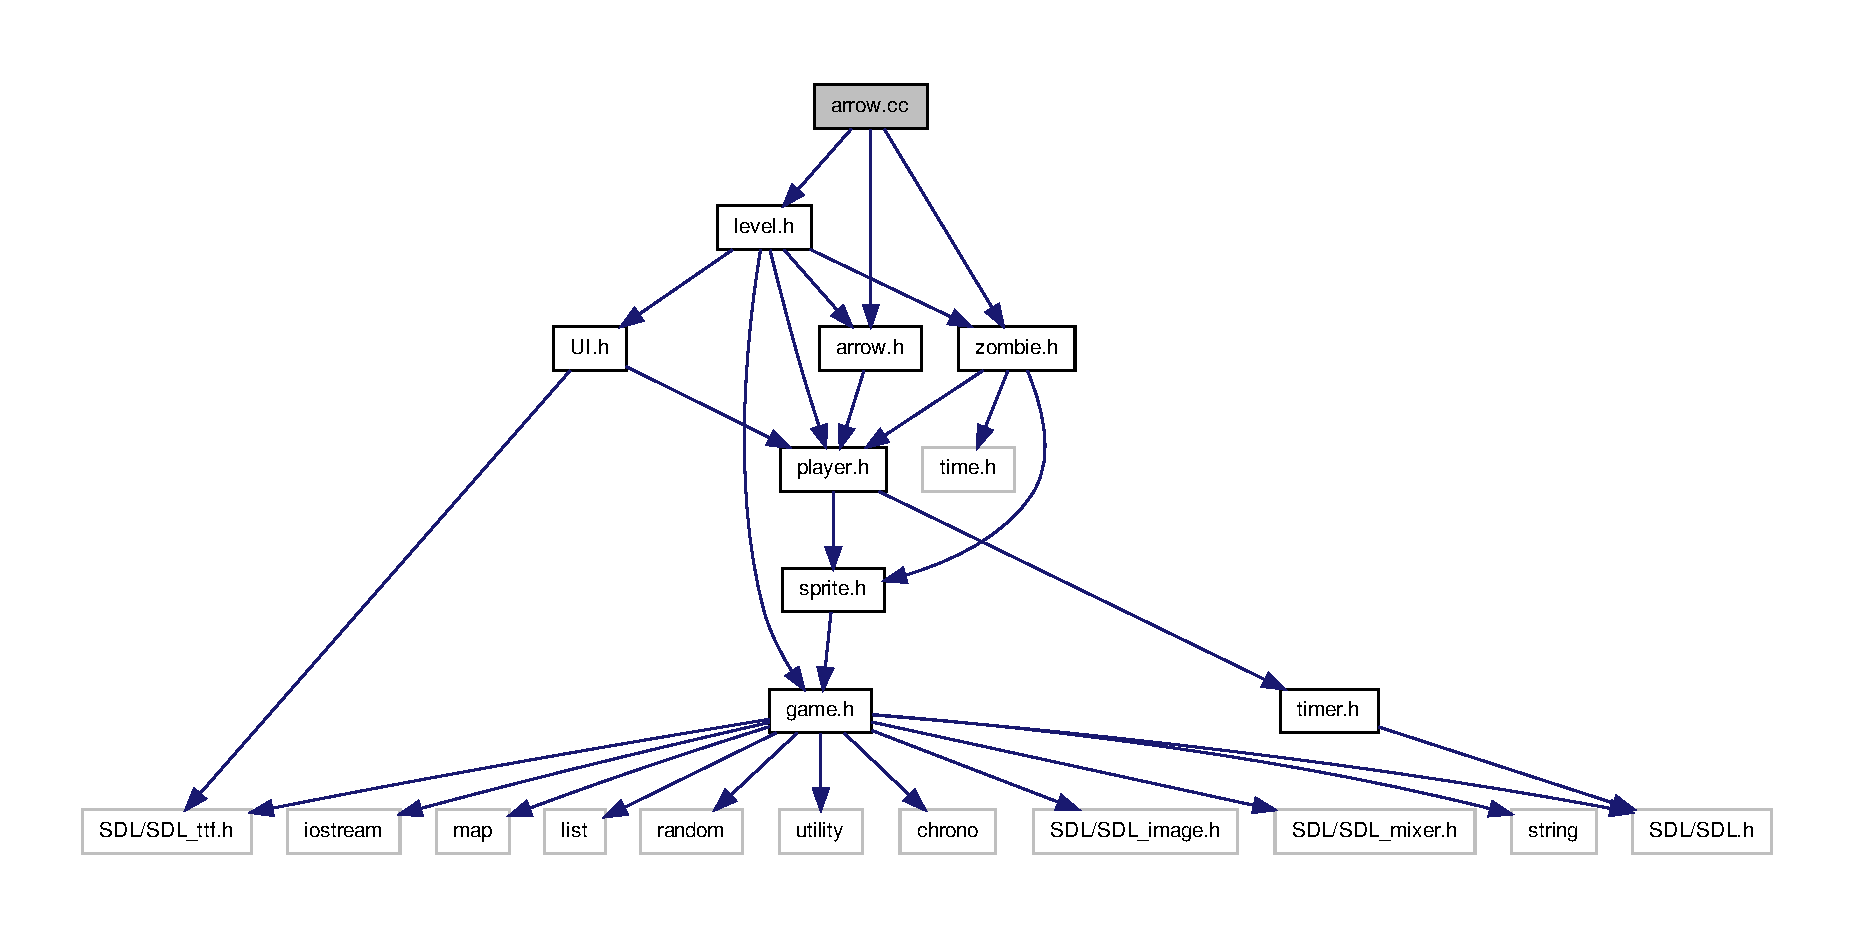
\includegraphics[width=350pt]{arrow_8cc__incl}
\end{center}
\end{figure}

\hypertarget{arrow_8h}{\section{arrow.\-h File Reference}
\label{arrow_8h}\index{arrow.\-h@{arrow.\-h}}
}
{\ttfamily \#include \char`\"{}player.\-h\char`\"{}}\\*
Include dependency graph for arrow.\-h\-:\nopagebreak
\begin{figure}[H]
\begin{center}
\leavevmode
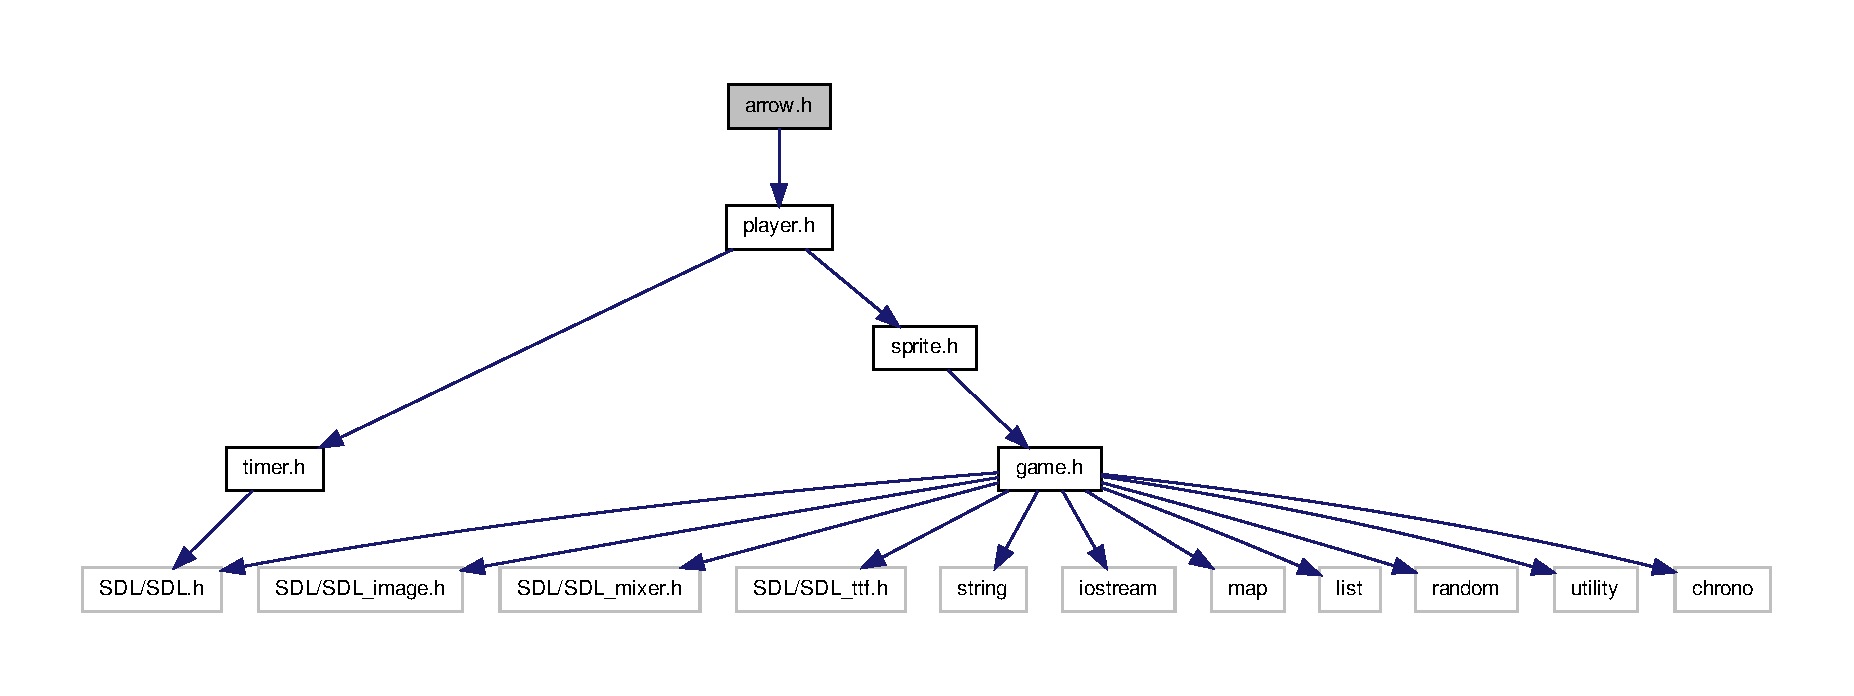
\includegraphics[width=350pt]{arrow_8h__incl}
\end{center}
\end{figure}
This graph shows which files directly or indirectly include this file\-:\nopagebreak
\begin{figure}[H]
\begin{center}
\leavevmode
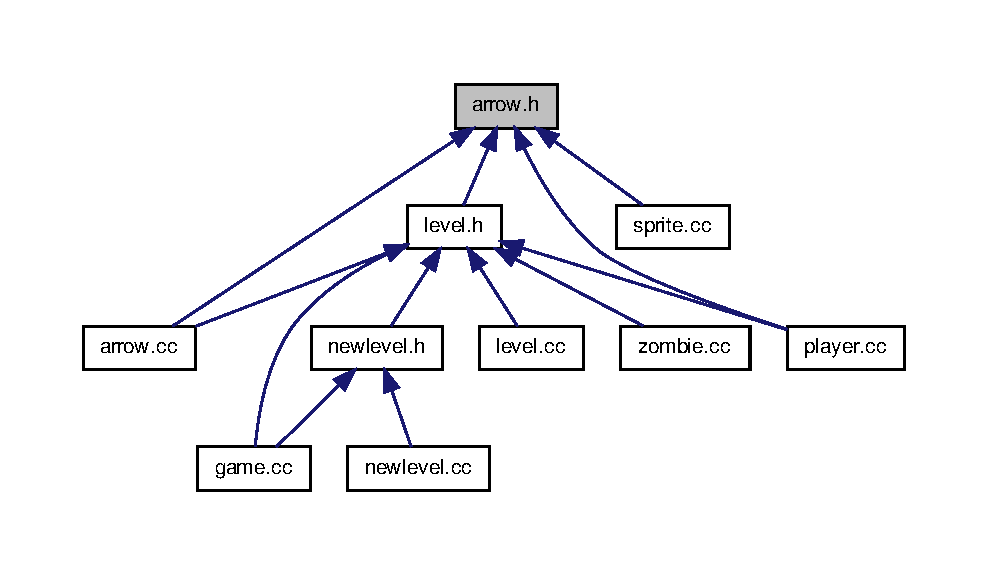
\includegraphics[width=350pt]{arrow_8h__dep__incl}
\end{center}
\end{figure}
\subsection*{Classes}
\begin{DoxyCompactItemize}
\item 
class \hyperlink{classArrow}{Arrow}
\end{DoxyCompactItemize}

\hypertarget{game_8cc}{\section{game.\-cc File Reference}
\label{game_8cc}\index{game.\-cc@{game.\-cc}}
}
{\ttfamily \#include \char`\"{}game.\-h\char`\"{}}\\*
{\ttfamily \#include \char`\"{}timer.\-h\char`\"{}}\\*
{\ttfamily \#include \char`\"{}menu.\-h\char`\"{}}\\*
{\ttfamily \#include \char`\"{}level.\-h\char`\"{}}\\*
{\ttfamily \#include \char`\"{}newlevel.\-h\char`\"{}}\\*
Include dependency graph for game.\-cc\-:\nopagebreak
\begin{figure}[H]
\begin{center}
\leavevmode
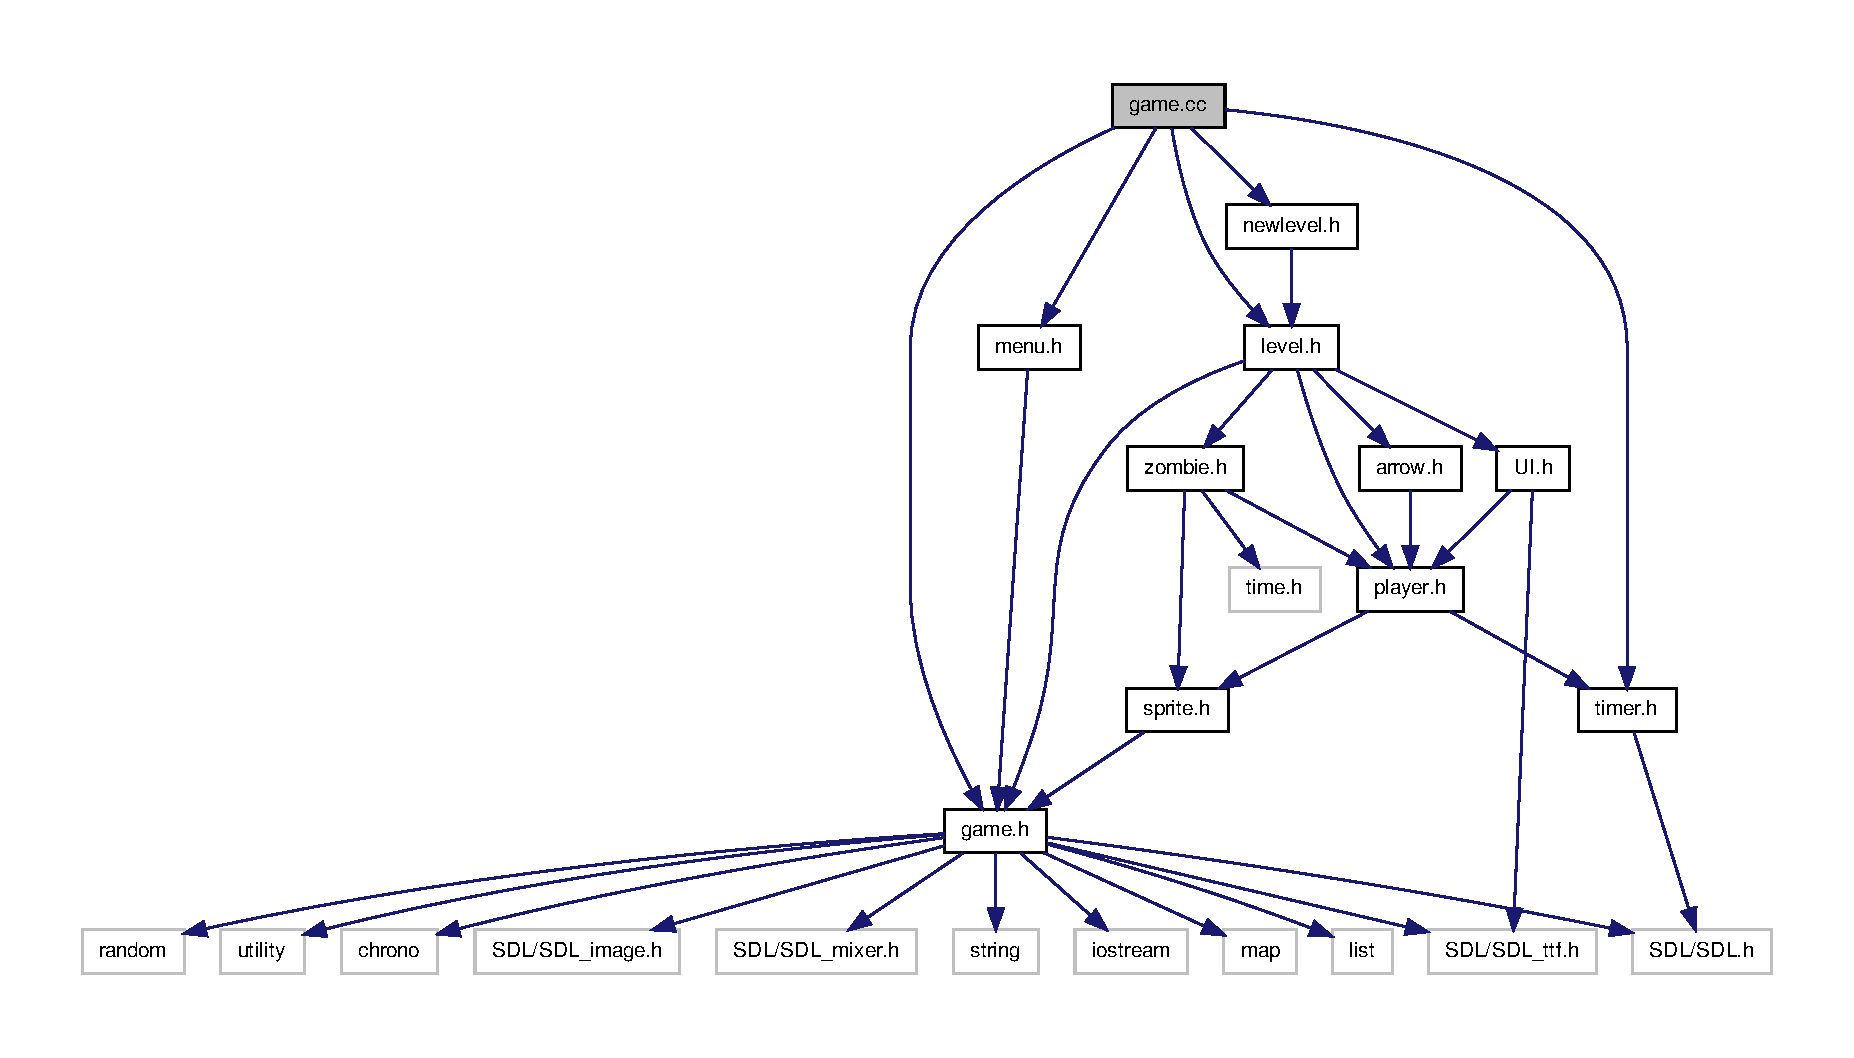
\includegraphics[width=350pt]{game_8cc__incl}
\end{center}
\end{figure}

\hypertarget{game_8h}{\section{game.\-h File Reference}
\label{game_8h}\index{game.\-h@{game.\-h}}
}
{\ttfamily \#include $<$S\-D\-L/\-S\-D\-L.\-h$>$}\\*
{\ttfamily \#include $<$S\-D\-L/\-S\-D\-L\-\_\-image.\-h$>$}\\*
{\ttfamily \#include $<$S\-D\-L/\-S\-D\-L\-\_\-mixer.\-h$>$}\\*
{\ttfamily \#include $<$S\-D\-L/\-S\-D\-L\-\_\-ttf.\-h$>$}\\*
{\ttfamily \#include $<$string$>$}\\*
{\ttfamily \#include $<$iostream$>$}\\*
{\ttfamily \#include $<$map$>$}\\*
{\ttfamily \#include $<$list$>$}\\*
{\ttfamily \#include $<$random$>$}\\*
{\ttfamily \#include $<$utility$>$}\\*
{\ttfamily \#include $<$chrono$>$}\\*
Include dependency graph for game.\-h\-:\nopagebreak
\begin{figure}[H]
\begin{center}
\leavevmode
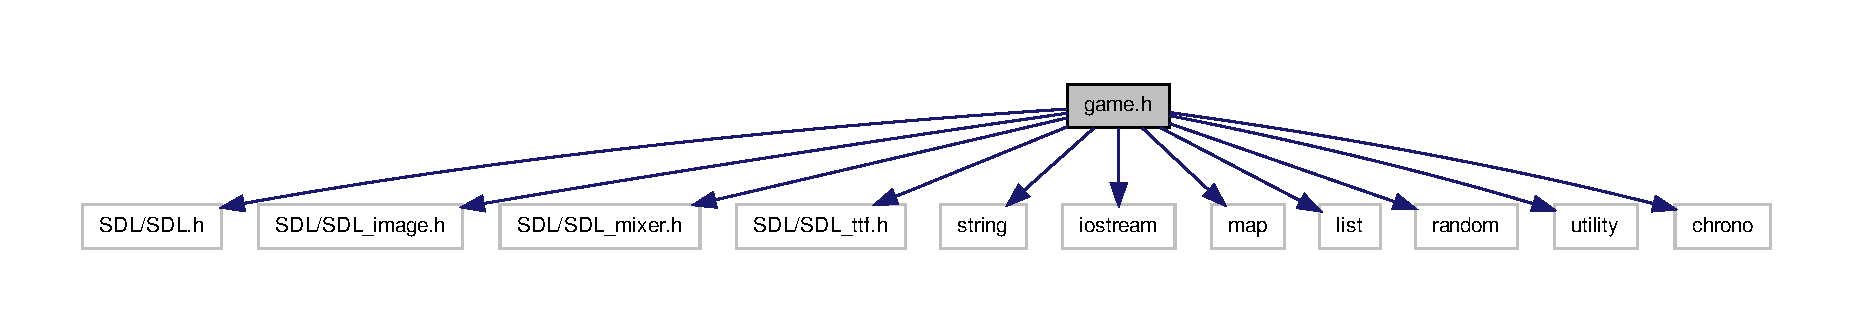
\includegraphics[width=350pt]{game_8h__incl}
\end{center}
\end{figure}
This graph shows which files directly or indirectly include this file\-:\nopagebreak
\begin{figure}[H]
\begin{center}
\leavevmode
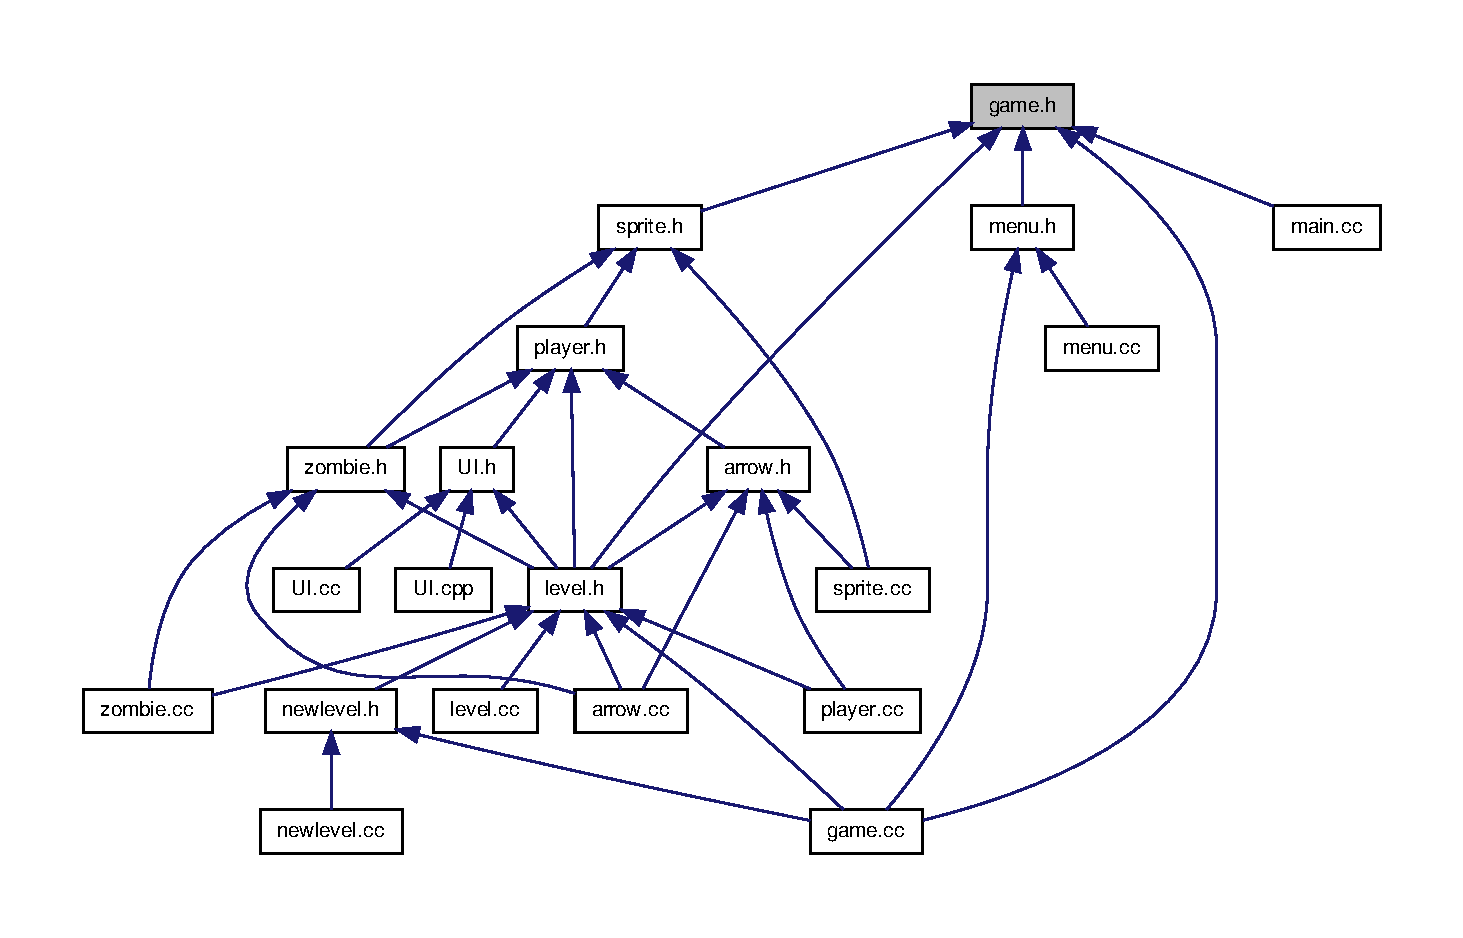
\includegraphics[width=350pt]{game_8h__dep__incl}
\end{center}
\end{figure}
\subsection*{Classes}
\begin{DoxyCompactItemize}
\item 
class \hyperlink{classGame}{Game}
\end{DoxyCompactItemize}

\hypertarget{level_8cc}{\section{level.\-cc File Reference}
\label{level_8cc}\index{level.\-cc@{level.\-cc}}
}
{\ttfamily \#include \char`\"{}level.\-h\char`\"{}}\\*
Include dependency graph for level.\-cc\-:\nopagebreak
\begin{figure}[H]
\begin{center}
\leavevmode
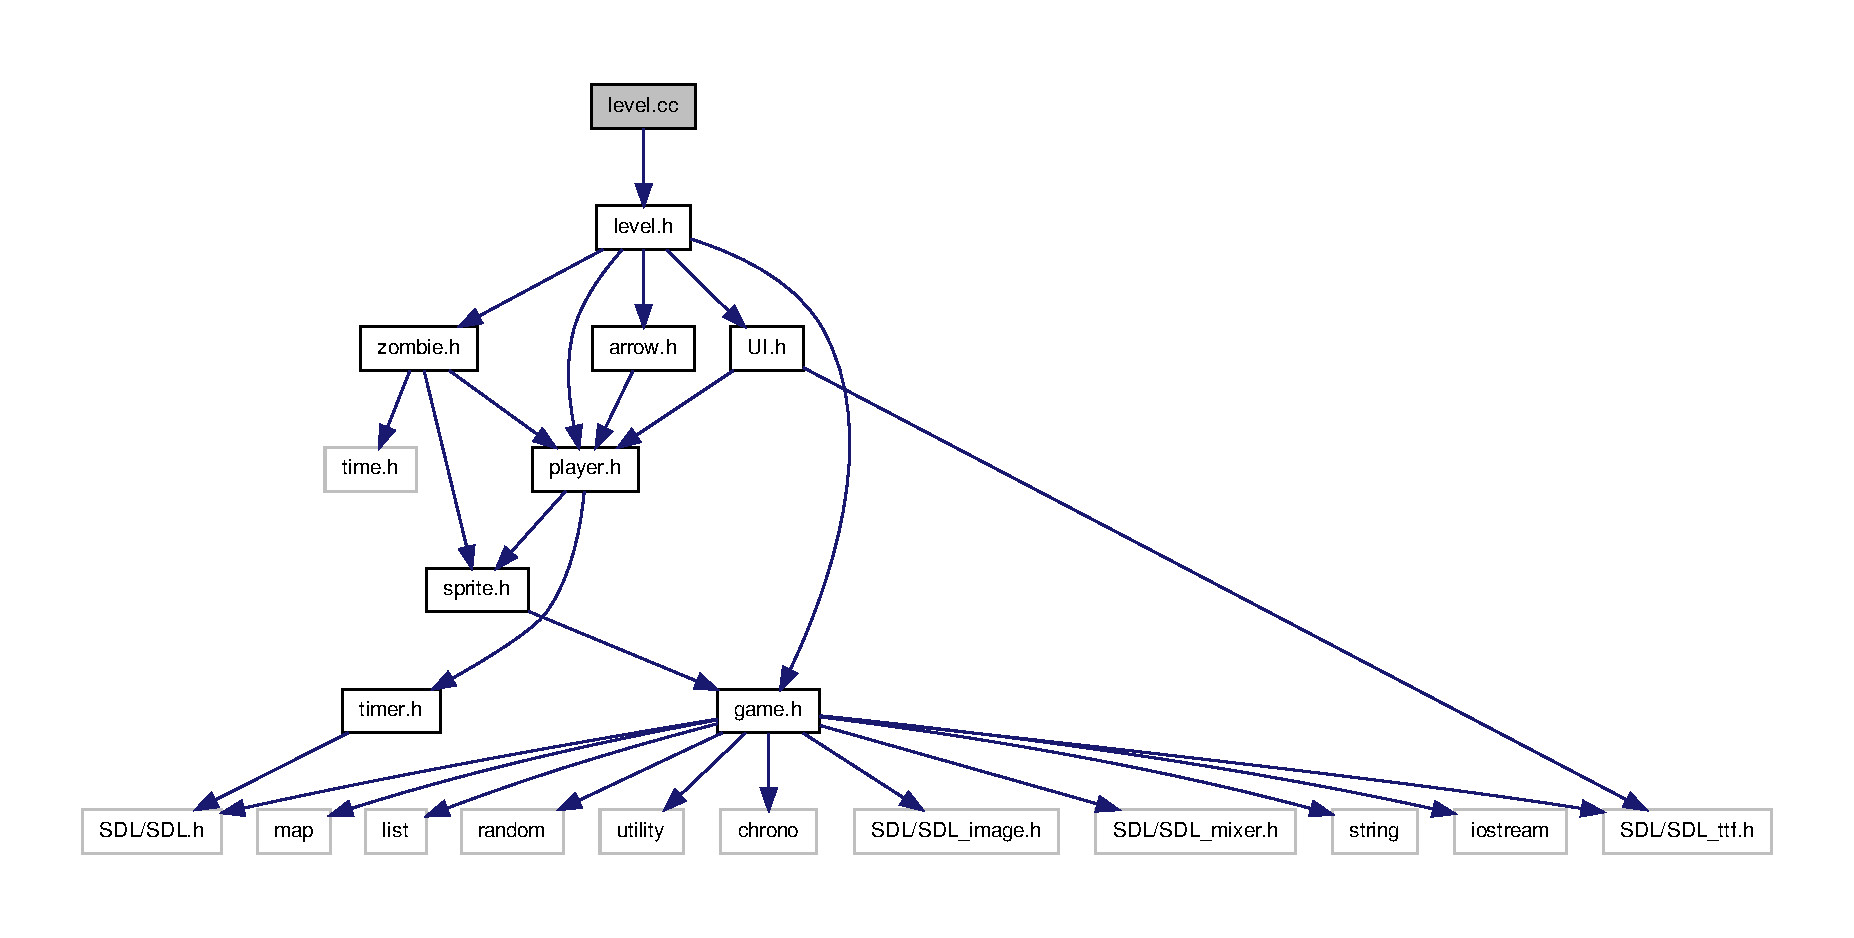
\includegraphics[width=350pt]{level_8cc__incl}
\end{center}
\end{figure}

\hypertarget{level_8h}{\section{level.\-h File Reference}
\label{level_8h}\index{level.\-h@{level.\-h}}
}
{\ttfamily \#include \char`\"{}game.\-h\char`\"{}}\\*
{\ttfamily \#include \char`\"{}player.\-h\char`\"{}}\\*
{\ttfamily \#include \char`\"{}zombie.\-h\char`\"{}}\\*
{\ttfamily \#include \char`\"{}arrow.\-h\char`\"{}}\\*
{\ttfamily \#include \char`\"{}U\-I.\-h\char`\"{}}\\*
Include dependency graph for level.\-h\-:\nopagebreak
\begin{figure}[H]
\begin{center}
\leavevmode
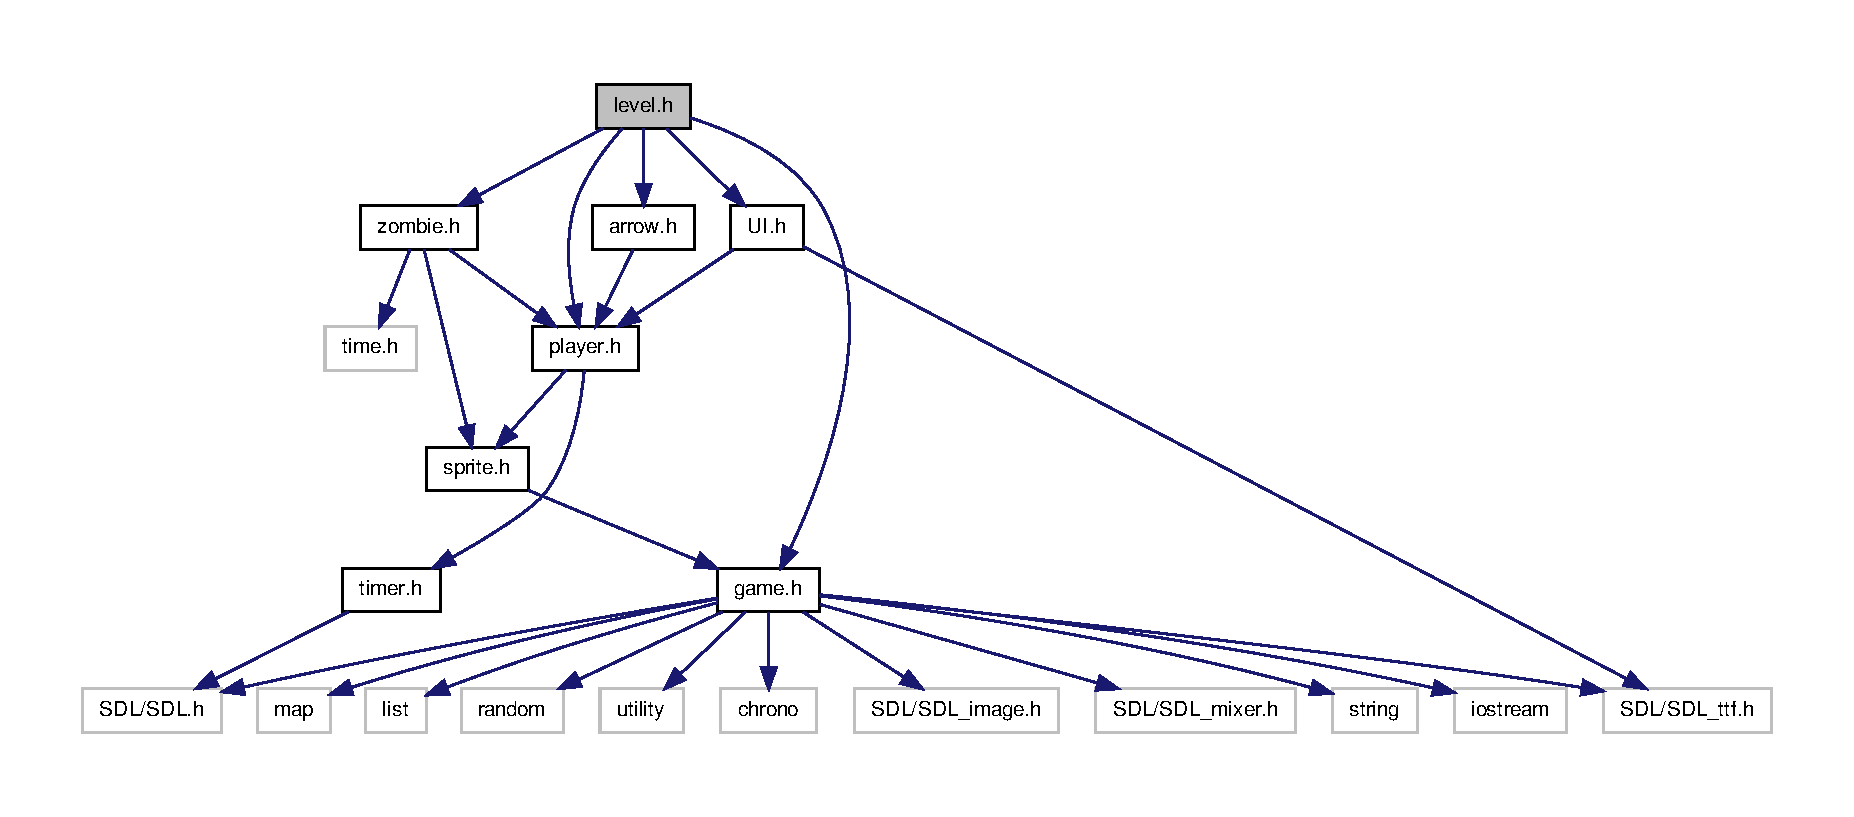
\includegraphics[width=350pt]{level_8h__incl}
\end{center}
\end{figure}
This graph shows which files directly or indirectly include this file\-:\nopagebreak
\begin{figure}[H]
\begin{center}
\leavevmode
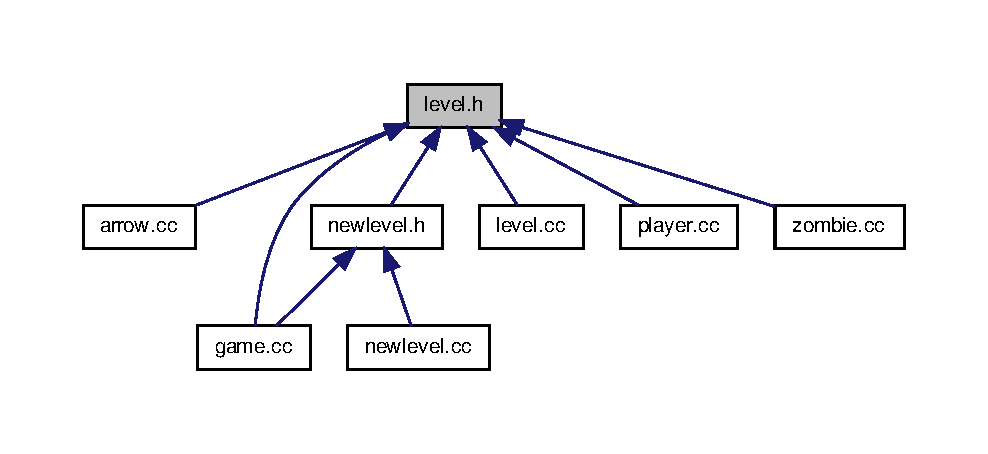
\includegraphics[width=350pt]{level_8h__dep__incl}
\end{center}
\end{figure}
\subsection*{Classes}
\begin{DoxyCompactItemize}
\item 
class \hyperlink{classLevel}{Level}
\item 
struct \hyperlink{structLevel_1_1Difficulty}{Level\-::\-Difficulty}
\end{DoxyCompactItemize}

\hypertarget{main_8cc}{\section{main.\-cc File Reference}
\label{main_8cc}\index{main.\-cc@{main.\-cc}}
}
{\ttfamily \#include $<$iostream$>$}\\*
{\ttfamily \#include \char`\"{}game.\-h\char`\"{}}\\*
Include dependency graph for main.\-cc\-:\nopagebreak
\begin{figure}[H]
\begin{center}
\leavevmode
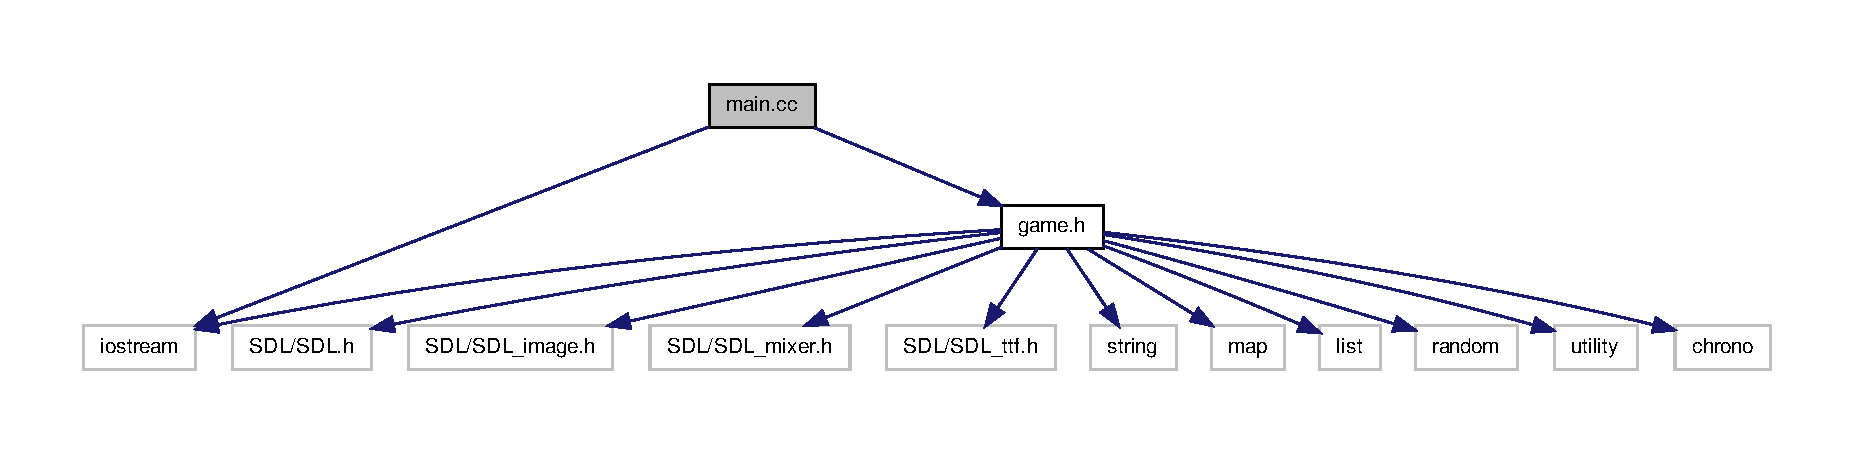
\includegraphics[width=350pt]{main_8cc__incl}
\end{center}
\end{figure}
\subsection*{Functions}
\begin{DoxyCompactItemize}
\item 
int \hyperlink{main_8cc_a0ddf1224851353fc92bfbff6f499fa97}{main} (int argc, char $\ast$argv\mbox{[}$\,$\mbox{]})
\end{DoxyCompactItemize}


\subsection{Function Documentation}
\hypertarget{main_8cc_a0ddf1224851353fc92bfbff6f499fa97}{\index{main.\-cc@{main.\-cc}!main@{main}}
\index{main@{main}!main.cc@{main.\-cc}}
\subsubsection[{main}]{\setlength{\rightskip}{0pt plus 5cm}int main (
\begin{DoxyParamCaption}
\item[{int}]{argc, }
\item[{char $\ast$}]{argv\mbox{[}$\,$\mbox{]}}
\end{DoxyParamCaption}
)}}\label{main_8cc_a0ddf1224851353fc92bfbff6f499fa97}

\hypertarget{menu_8cc}{\section{menu.\-cc File Reference}
\label{menu_8cc}\index{menu.\-cc@{menu.\-cc}}
}
{\ttfamily \#include \char`\"{}menu.\-h\char`\"{}}\\*
Include dependency graph for menu.\-cc\-:\nopagebreak
\begin{figure}[H]
\begin{center}
\leavevmode
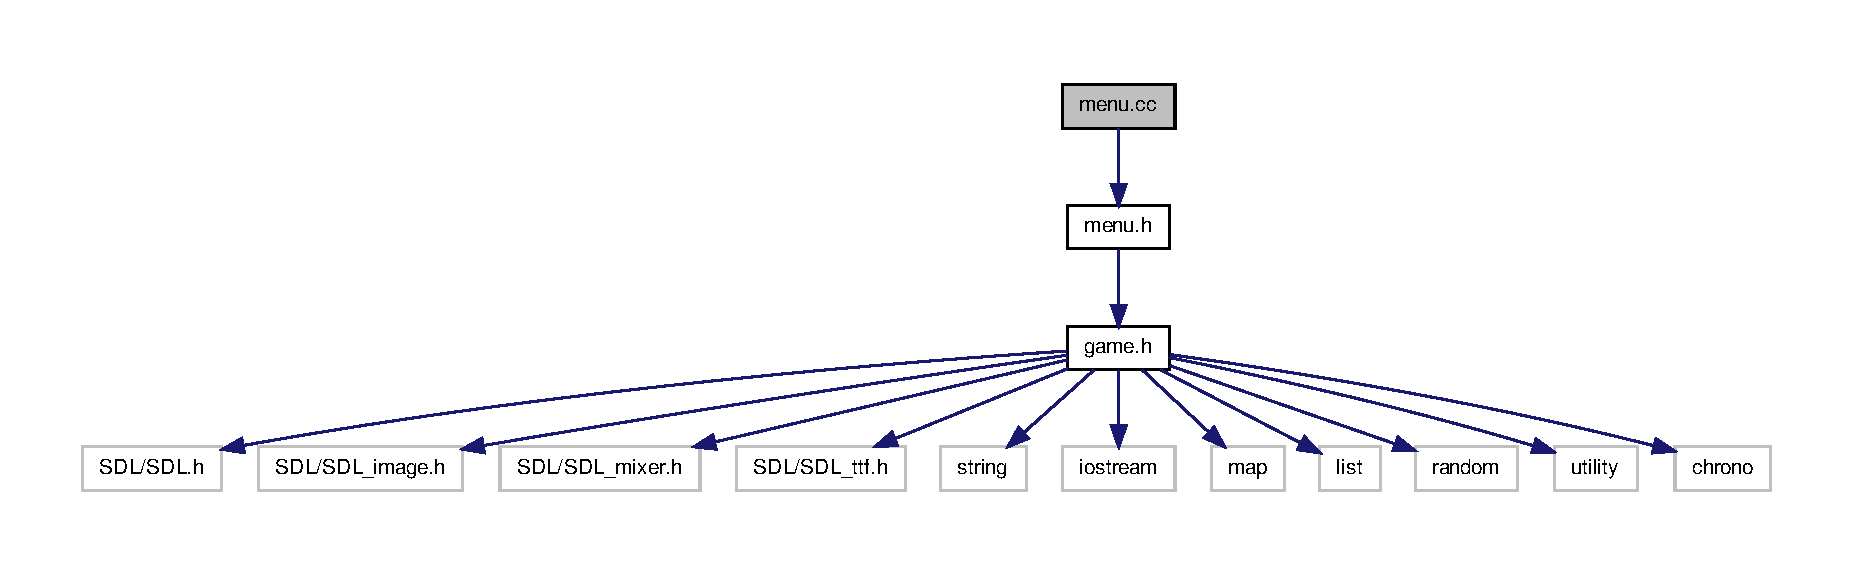
\includegraphics[width=350pt]{menu_8cc__incl}
\end{center}
\end{figure}

\hypertarget{menu_8h}{\section{menu.\-h File Reference}
\label{menu_8h}\index{menu.\-h@{menu.\-h}}
}
{\ttfamily \#include \char`\"{}game.\-h\char`\"{}}\\*
Include dependency graph for menu.\-h\-:\nopagebreak
\begin{figure}[H]
\begin{center}
\leavevmode
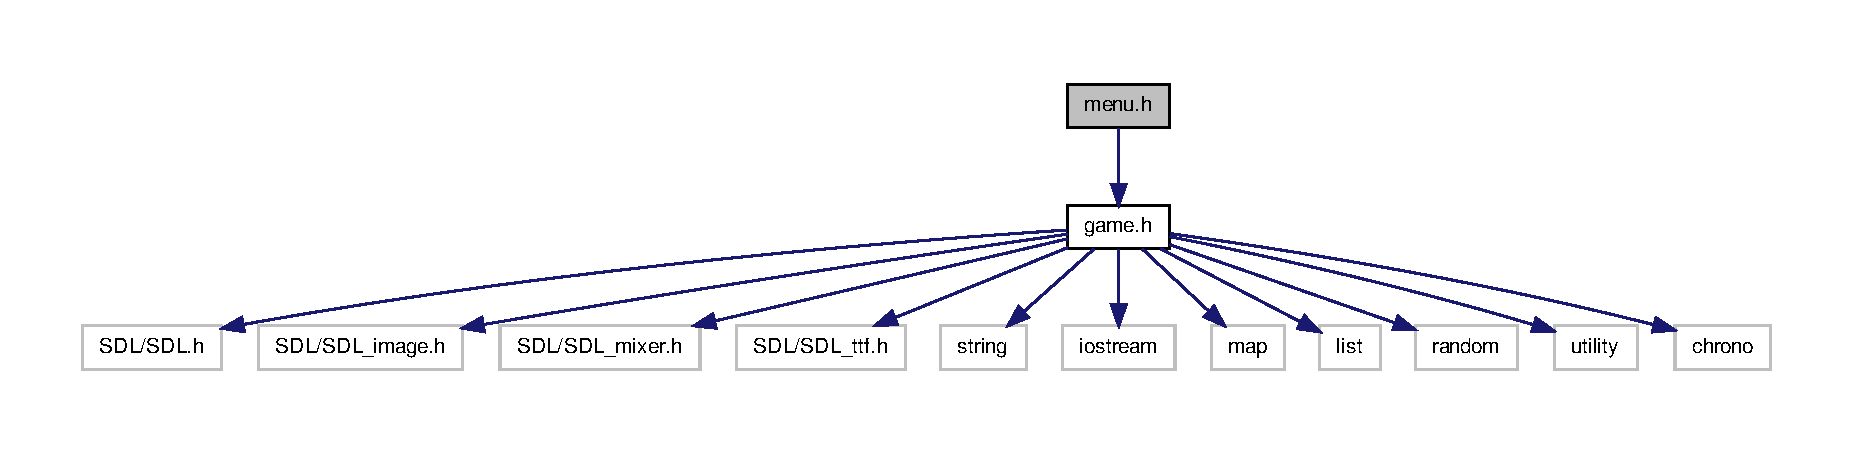
\includegraphics[width=350pt]{menu_8h__incl}
\end{center}
\end{figure}
This graph shows which files directly or indirectly include this file\-:\nopagebreak
\begin{figure}[H]
\begin{center}
\leavevmode
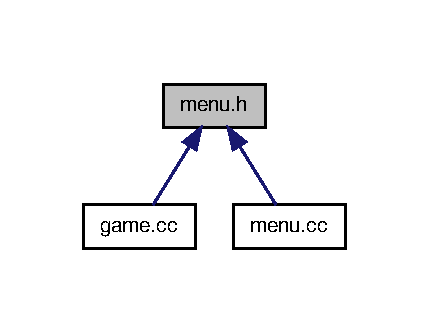
\includegraphics[width=206pt]{menu_8h__dep__incl}
\end{center}
\end{figure}
\subsection*{Classes}
\begin{DoxyCompactItemize}
\item 
class \hyperlink{classMenu}{Menu}
\end{DoxyCompactItemize}

\hypertarget{newlevel_8cc}{\section{newlevel.\-cc File Reference}
\label{newlevel_8cc}\index{newlevel.\-cc@{newlevel.\-cc}}
}
{\ttfamily \#include \char`\"{}newlevel.\-h\char`\"{}}\\*
{\ttfamily \#include $<$string$>$}\\*
{\ttfamily \#include $<$sstream$>$}\\*
{\ttfamily \#include $<$cctype$>$}\\*
Include dependency graph for newlevel.\-cc\-:\nopagebreak
\begin{figure}[H]
\begin{center}
\leavevmode
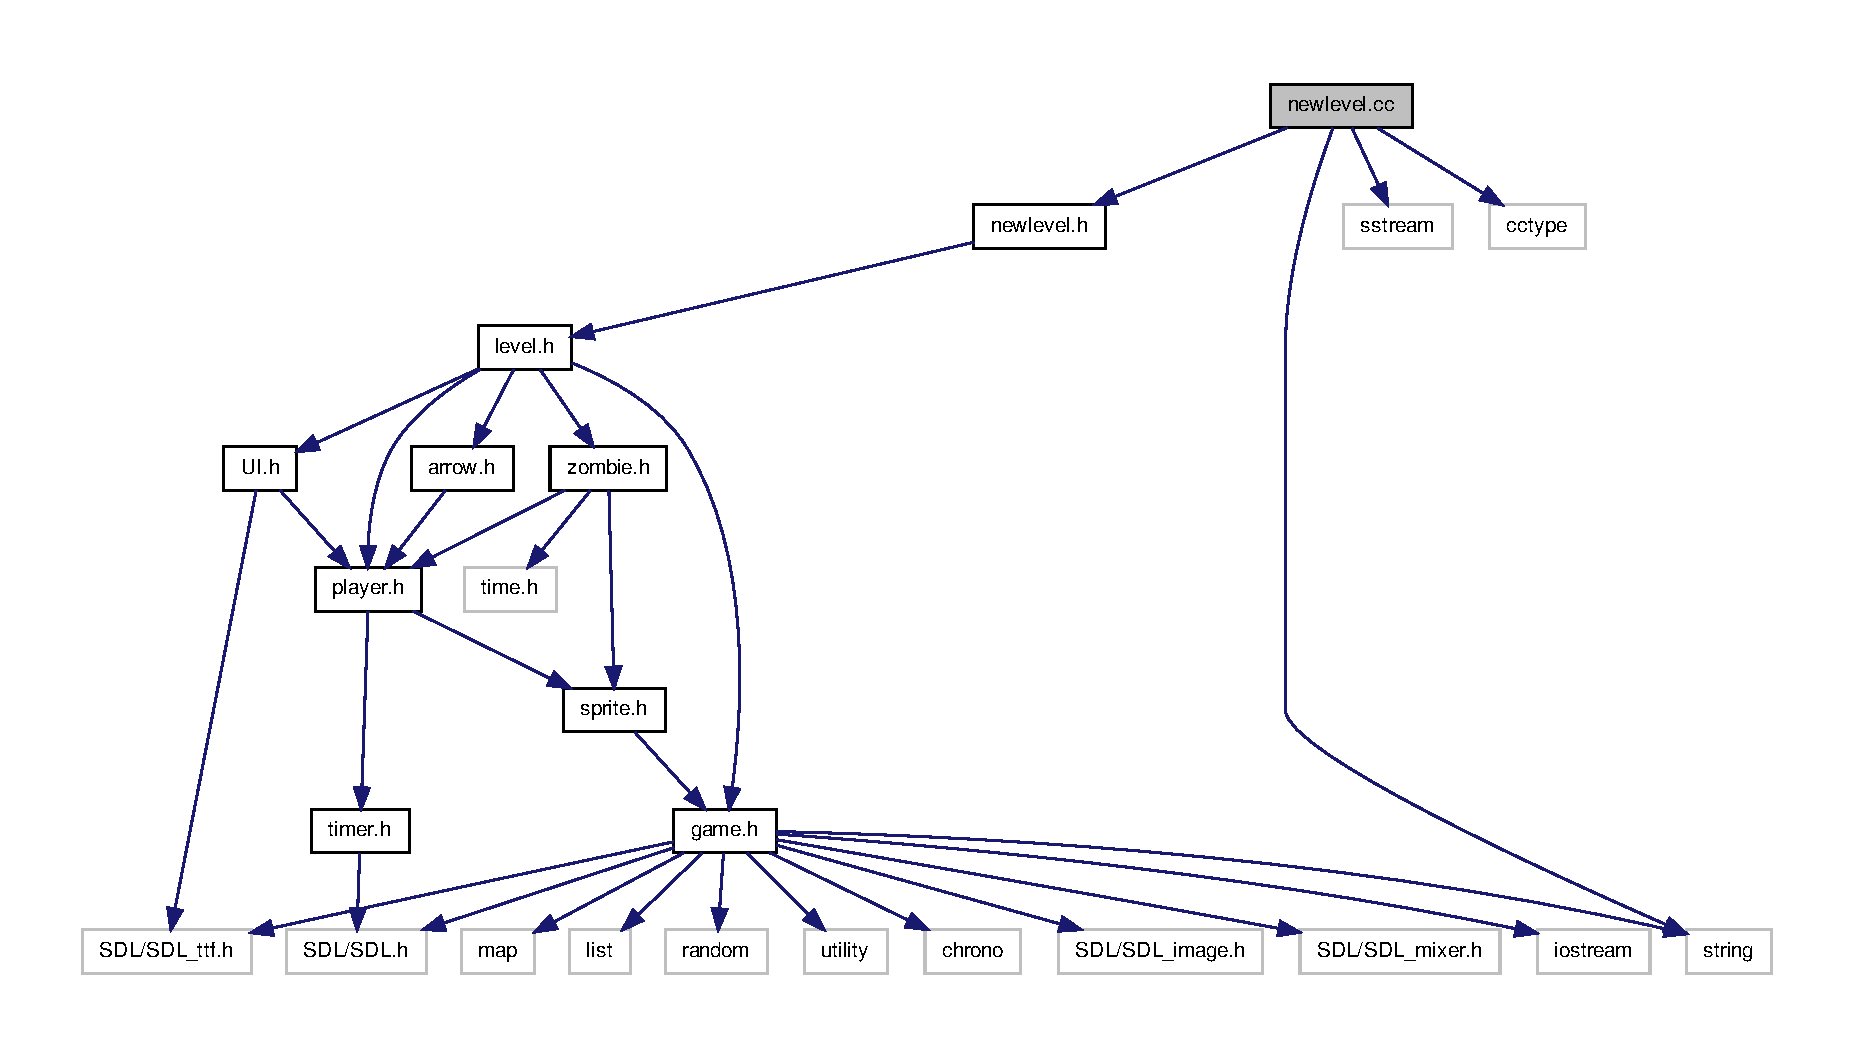
\includegraphics[width=350pt]{newlevel_8cc__incl}
\end{center}
\end{figure}

\hypertarget{newlevel_8h}{\section{newlevel.\-h File Reference}
\label{newlevel_8h}\index{newlevel.\-h@{newlevel.\-h}}
}
{\ttfamily \#include \char`\"{}level.\-h\char`\"{}}\\*
Include dependency graph for newlevel.\-h\-:\nopagebreak
\begin{figure}[H]
\begin{center}
\leavevmode
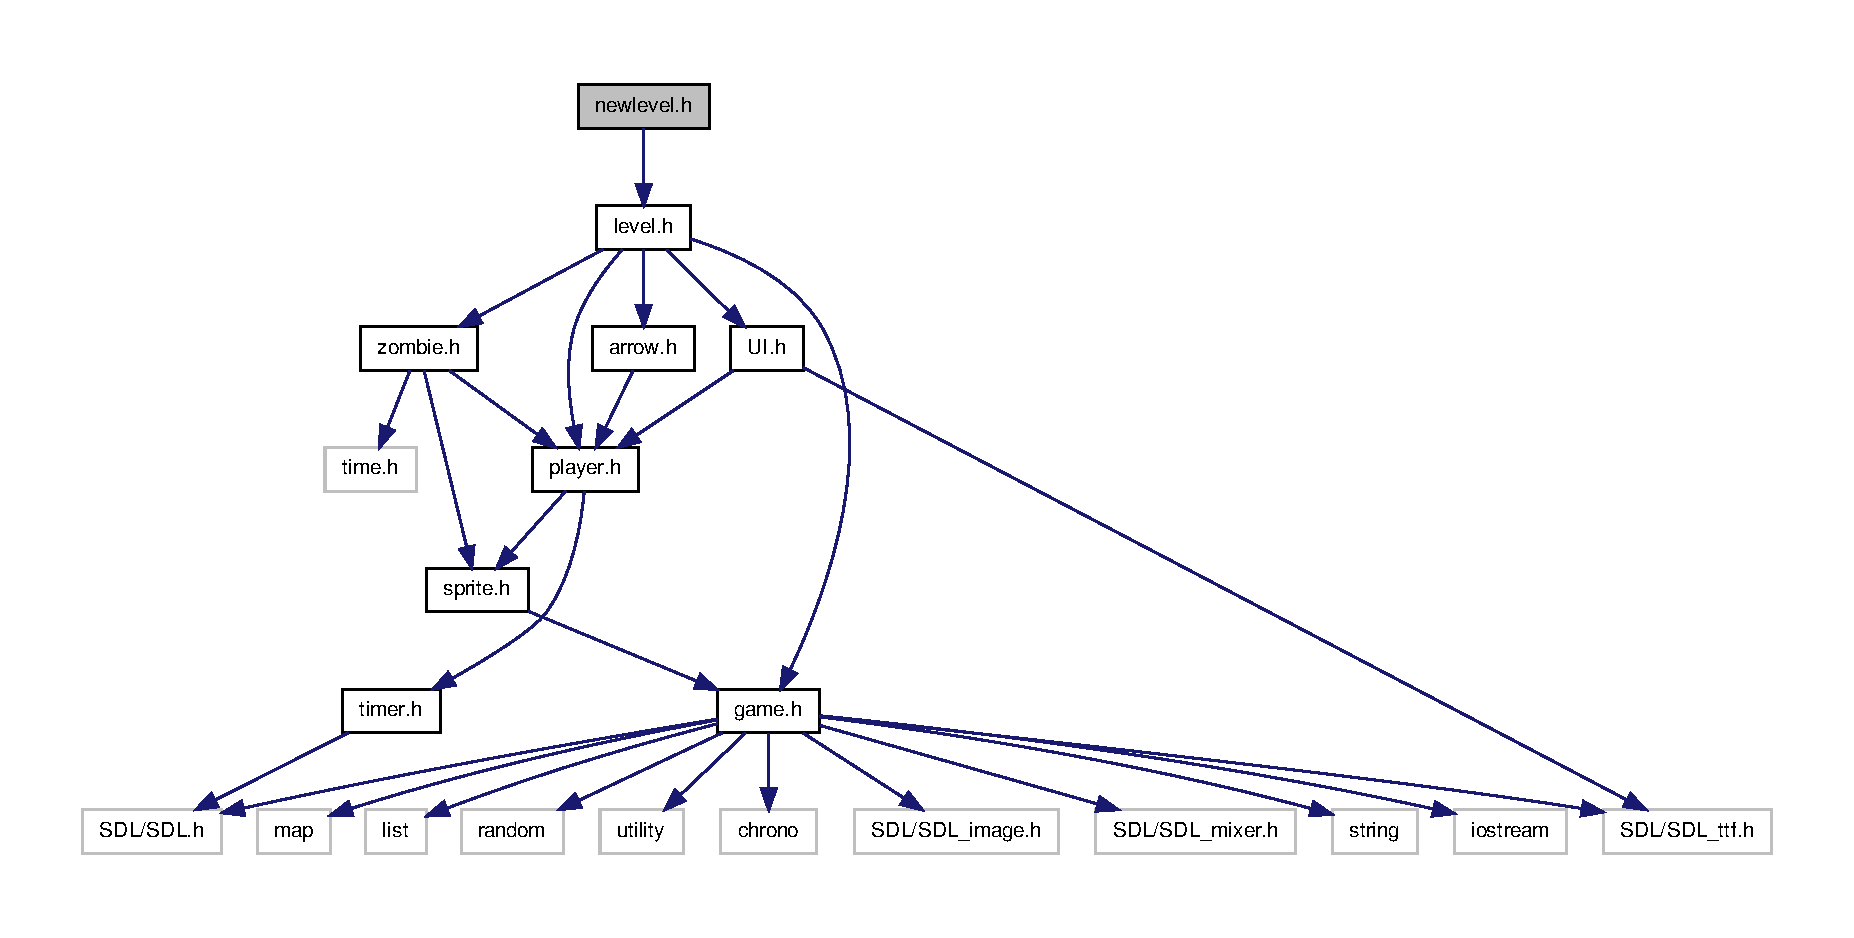
\includegraphics[width=350pt]{newlevel_8h__incl}
\end{center}
\end{figure}
This graph shows which files directly or indirectly include this file\-:\nopagebreak
\begin{figure}[H]
\begin{center}
\leavevmode
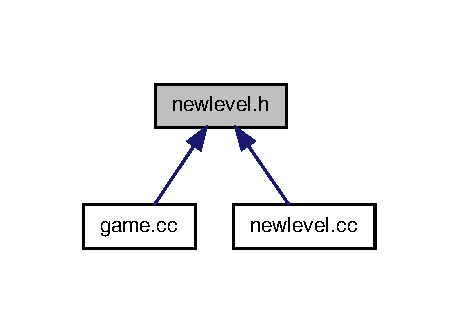
\includegraphics[width=220pt]{newlevel_8h__dep__incl}
\end{center}
\end{figure}
\subsection*{Classes}
\begin{DoxyCompactItemize}
\item 
class \hyperlink{classNewlevel}{Newlevel}
\end{DoxyCompactItemize}

\hypertarget{player_8cc}{\section{player.\-cc File Reference}
\label{player_8cc}\index{player.\-cc@{player.\-cc}}
}
{\ttfamily \#include \char`\"{}level.\-h\char`\"{}}\\*
{\ttfamily \#include \char`\"{}arrow.\-h\char`\"{}}\\*
Include dependency graph for player.\-cc\-:\nopagebreak
\begin{figure}[H]
\begin{center}
\leavevmode
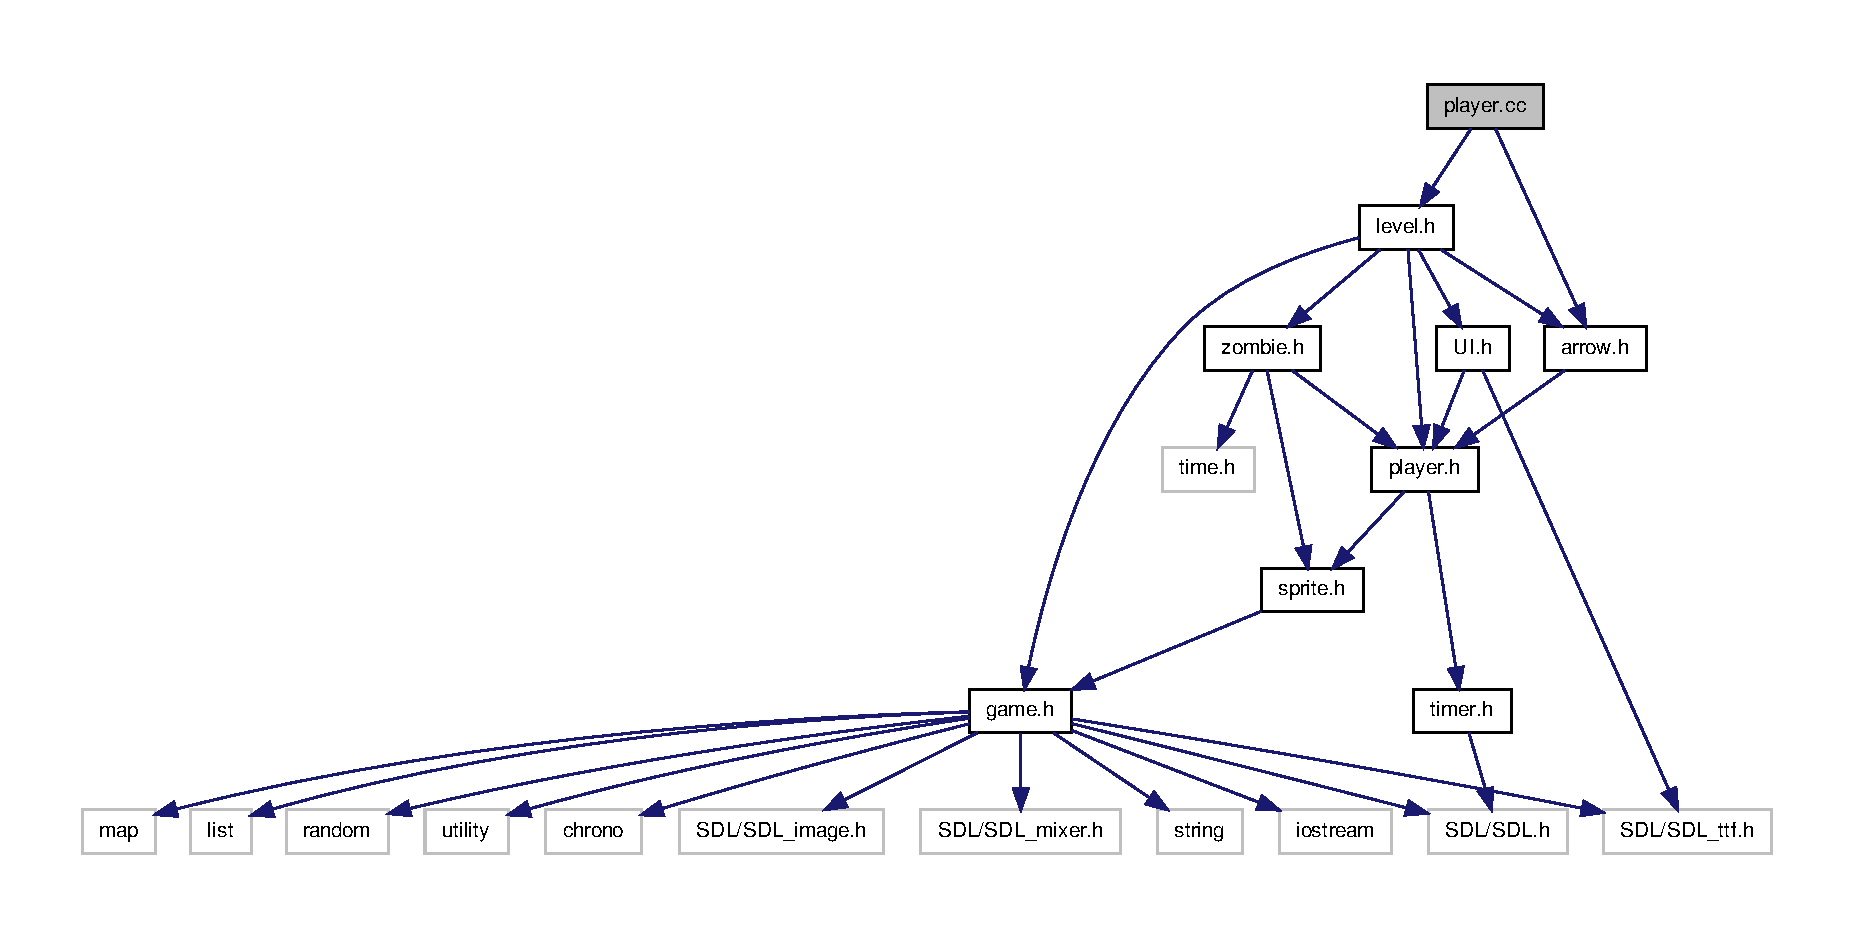
\includegraphics[width=350pt]{player_8cc__incl}
\end{center}
\end{figure}

\hypertarget{player_8h}{\section{player.\-h File Reference}
\label{player_8h}\index{player.\-h@{player.\-h}}
}
{\ttfamily \#include \char`\"{}sprite.\-h\char`\"{}}\\*
{\ttfamily \#include \char`\"{}timer.\-h\char`\"{}}\\*
Include dependency graph for player.\-h\-:\nopagebreak
\begin{figure}[H]
\begin{center}
\leavevmode
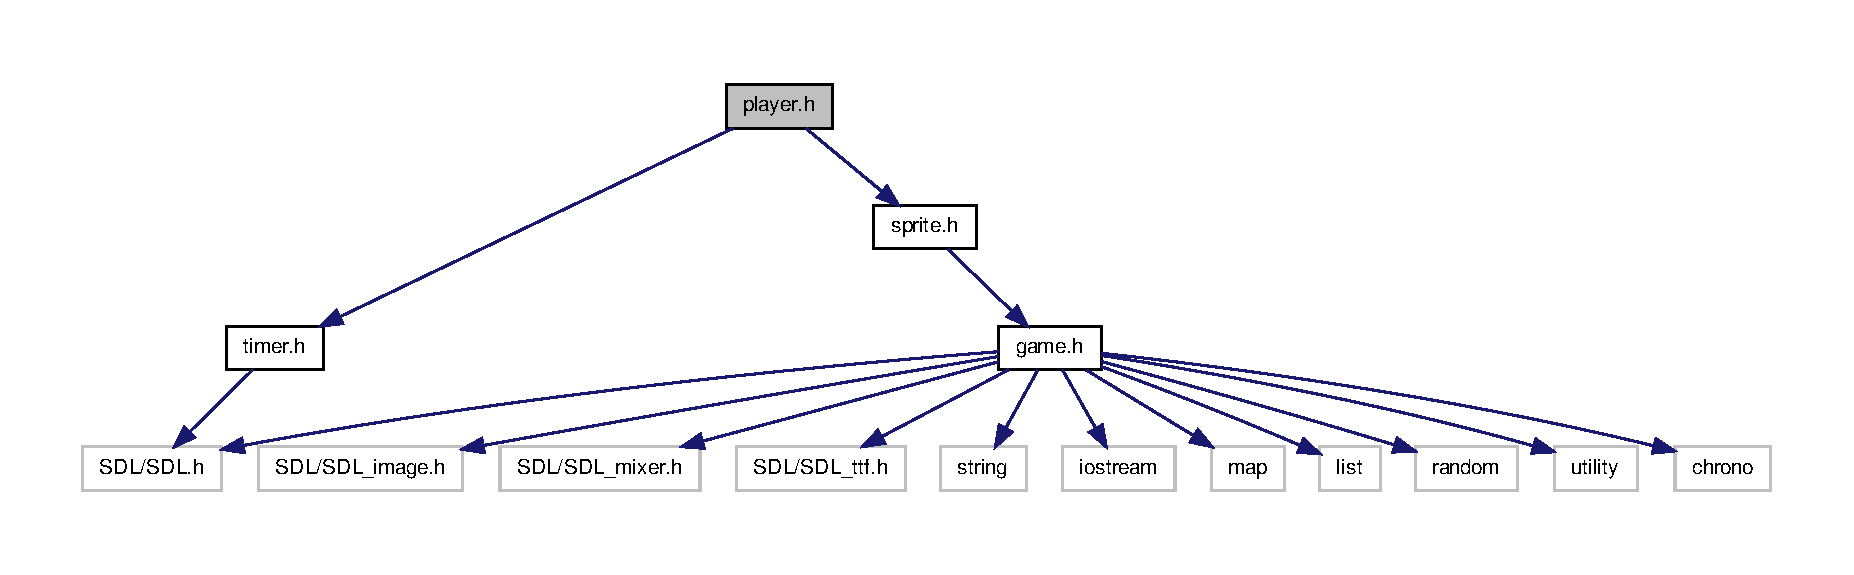
\includegraphics[width=350pt]{player_8h__incl}
\end{center}
\end{figure}
This graph shows which files directly or indirectly include this file\-:\nopagebreak
\begin{figure}[H]
\begin{center}
\leavevmode
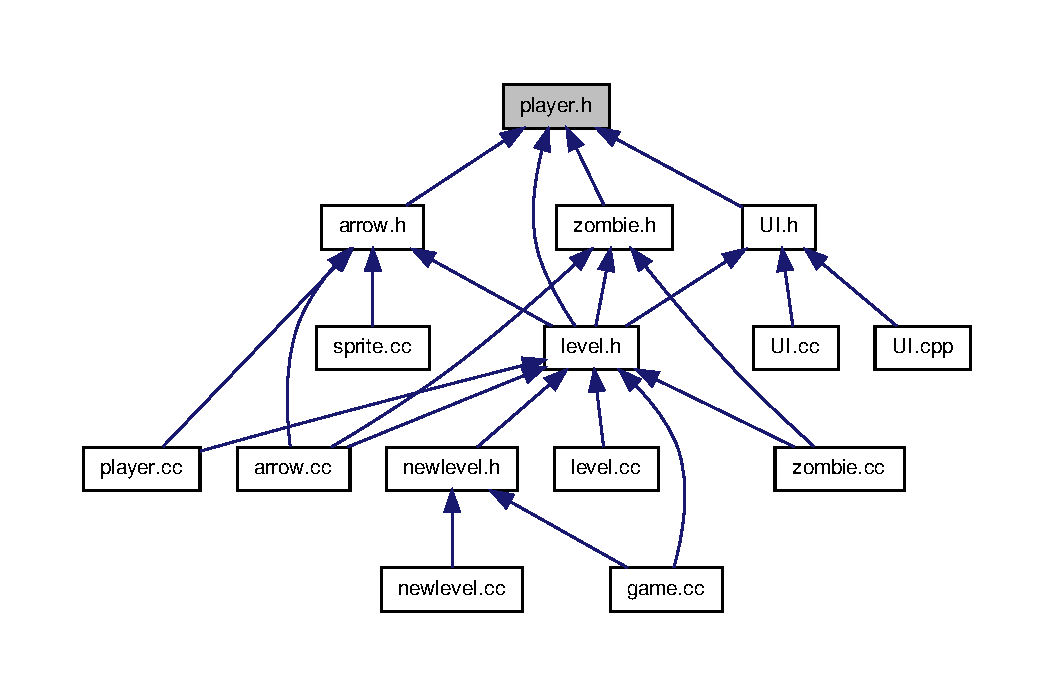
\includegraphics[width=350pt]{player_8h__dep__incl}
\end{center}
\end{figure}
\subsection*{Classes}
\begin{DoxyCompactItemize}
\item 
class \hyperlink{classPlayer}{Player}
\end{DoxyCompactItemize}

\hypertarget{sprite_8cc}{\section{sprite.\-cc File Reference}
\label{sprite_8cc}\index{sprite.\-cc@{sprite.\-cc}}
}
{\ttfamily \#include \char`\"{}arrow.\-h\char`\"{}}\\*
{\ttfamily \#include \char`\"{}sprite.\-h\char`\"{}}\\*
Include dependency graph for sprite.\-cc\-:\nopagebreak
\begin{figure}[H]
\begin{center}
\leavevmode
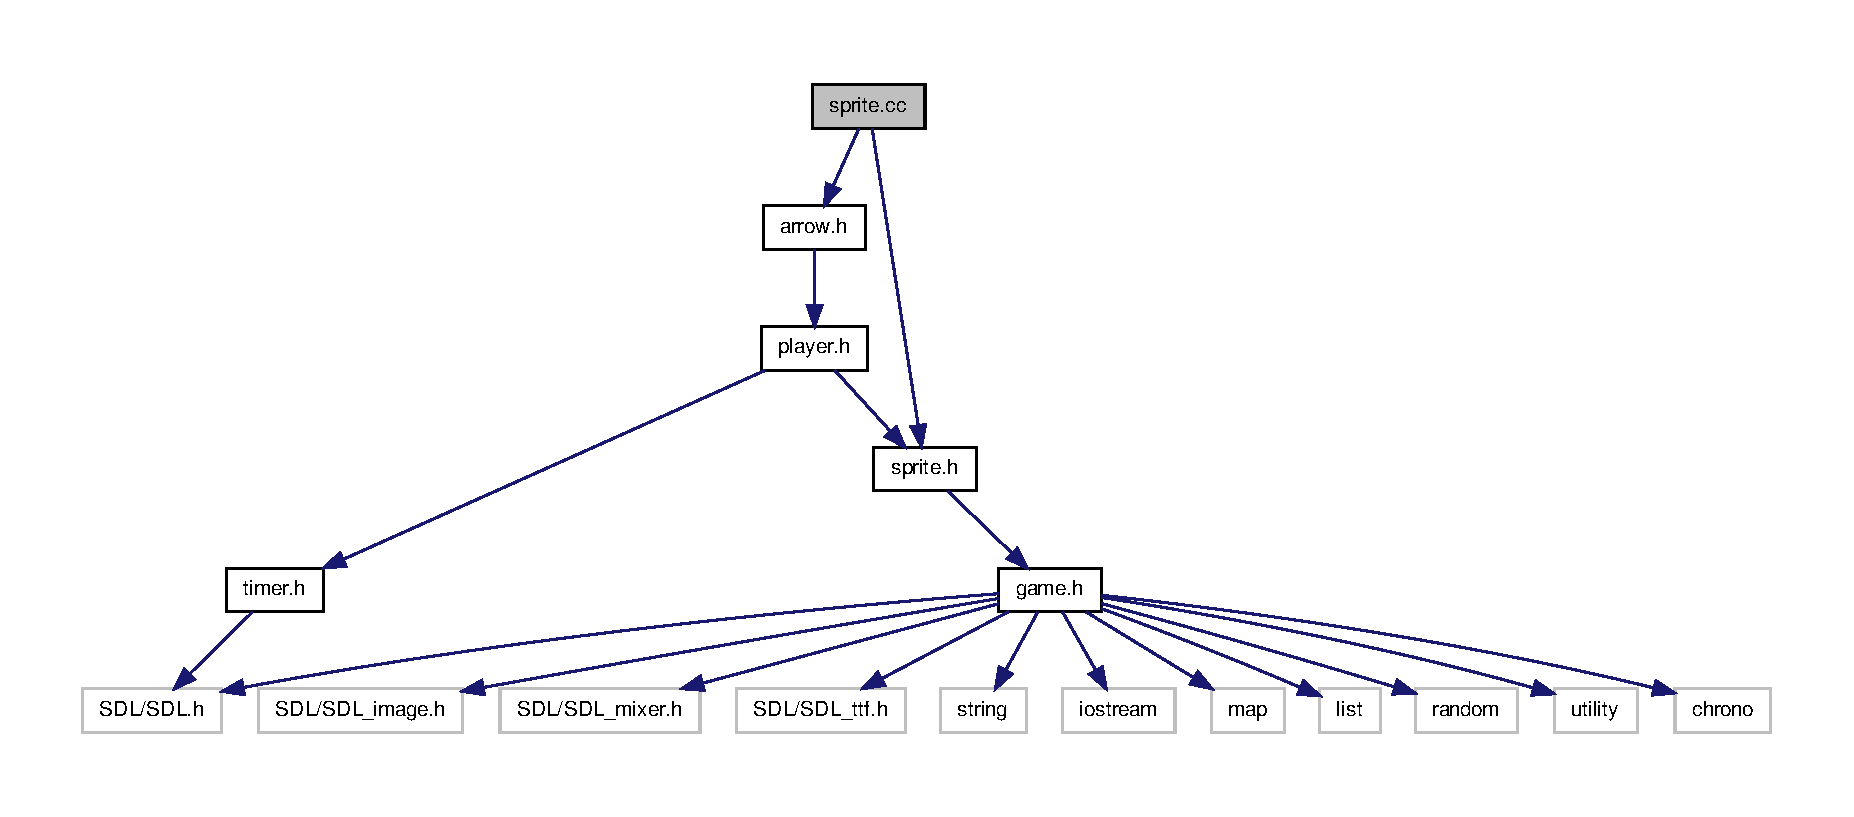
\includegraphics[width=350pt]{sprite_8cc__incl}
\end{center}
\end{figure}

\hypertarget{sprite_8h}{\section{sprite.\-h File Reference}
\label{sprite_8h}\index{sprite.\-h@{sprite.\-h}}
}
{\ttfamily \#include \char`\"{}game.\-h\char`\"{}}\\*
Include dependency graph for sprite.\-h\-:\nopagebreak
\begin{figure}[H]
\begin{center}
\leavevmode
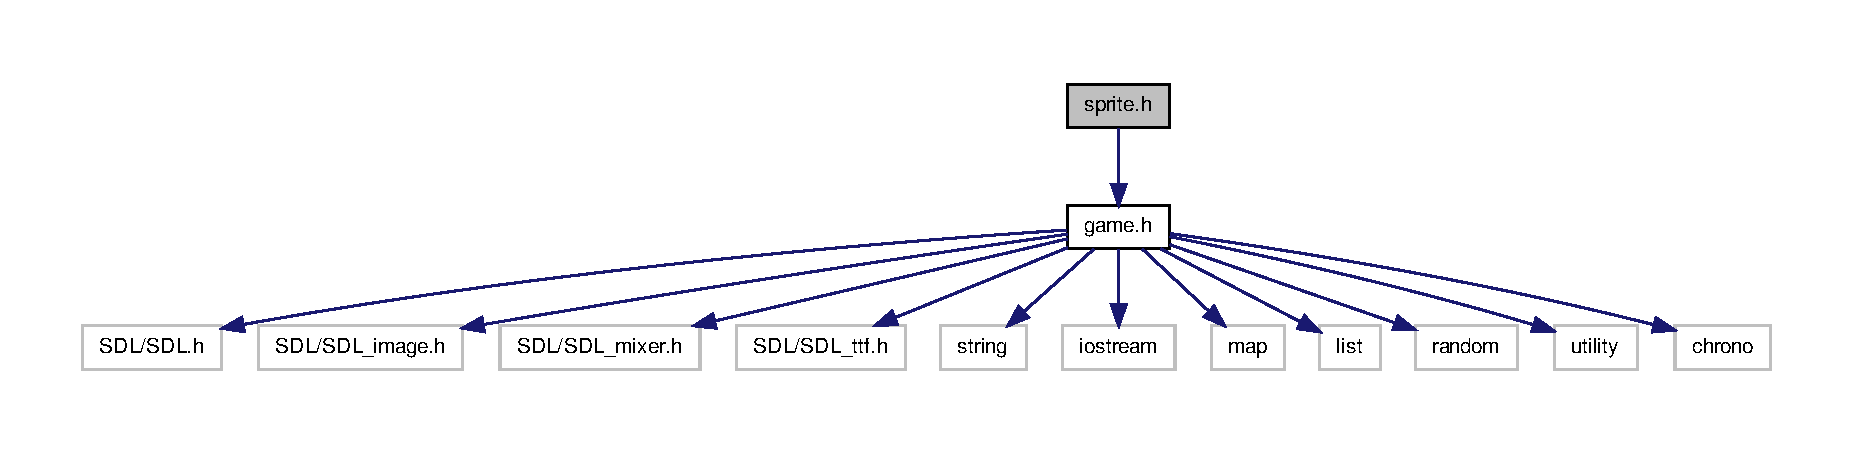
\includegraphics[width=350pt]{sprite_8h__incl}
\end{center}
\end{figure}
This graph shows which files directly or indirectly include this file\-:\nopagebreak
\begin{figure}[H]
\begin{center}
\leavevmode
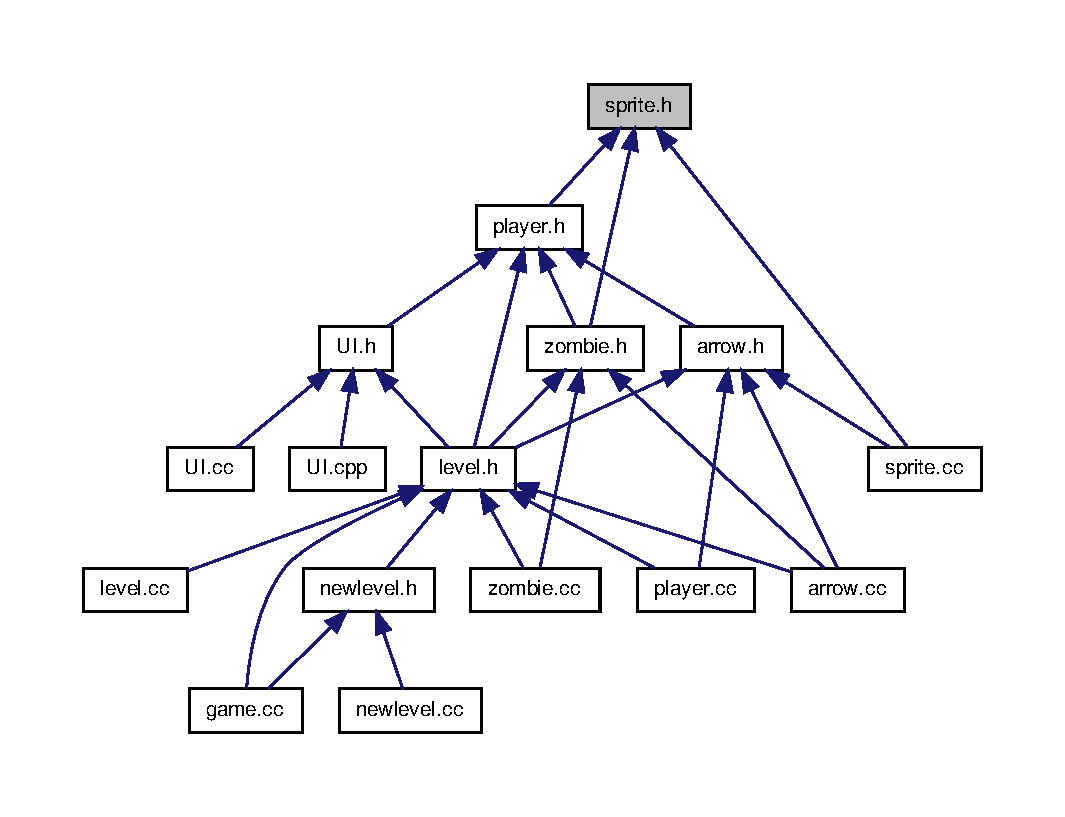
\includegraphics[width=350pt]{sprite_8h__dep__incl}
\end{center}
\end{figure}
\subsection*{Classes}
\begin{DoxyCompactItemize}
\item 
class \hyperlink{classSprite}{Sprite}
\end{DoxyCompactItemize}
\subsection*{Typedefs}
\begin{DoxyCompactItemize}
\item 
using \hyperlink{sprite_8h_a4e660753b3d87694743ccaf2bbc9150a}{animation\-Table} = std\-::map$<$ std\-::string, std\-::pair$<$ int, int $>$$>$
\end{DoxyCompactItemize}


\subsection{Typedef Documentation}
\hypertarget{sprite_8h_a4e660753b3d87694743ccaf2bbc9150a}{\index{sprite.\-h@{sprite.\-h}!animation\-Table@{animation\-Table}}
\index{animation\-Table@{animation\-Table}!sprite.h@{sprite.\-h}}
\subsubsection[{animation\-Table}]{\setlength{\rightskip}{0pt plus 5cm}using {\bf animation\-Table} =  std\-::map$<$std\-::string, std\-::pair$<$int, int$>$$>$}}\label{sprite_8h_a4e660753b3d87694743ccaf2bbc9150a}

\hypertarget{timer_8cc}{\section{timer.\-cc File Reference}
\label{timer_8cc}\index{timer.\-cc@{timer.\-cc}}
}
{\ttfamily \#include \char`\"{}timer.\-h\char`\"{}}\\*
Include dependency graph for timer.\-cc\-:\nopagebreak
\begin{figure}[H]
\begin{center}
\leavevmode
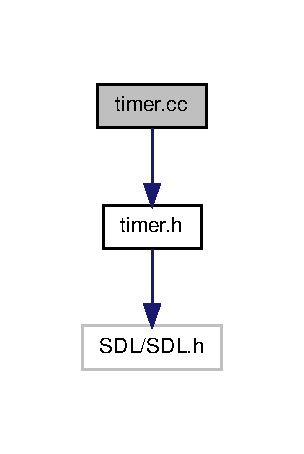
\includegraphics[width=146pt]{timer_8cc__incl}
\end{center}
\end{figure}

\hypertarget{timer_8h}{\section{timer.\-h File Reference}
\label{timer_8h}\index{timer.\-h@{timer.\-h}}
}
{\ttfamily \#include $<$S\-D\-L/\-S\-D\-L.\-h$>$}\\*
Include dependency graph for timer.\-h\-:\nopagebreak
\begin{figure}[H]
\begin{center}
\leavevmode
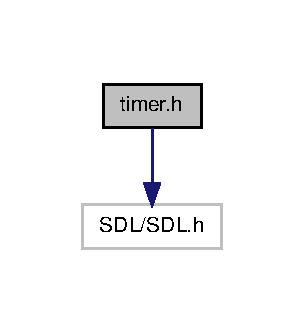
\includegraphics[width=146pt]{timer_8h__incl}
\end{center}
\end{figure}
This graph shows which files directly or indirectly include this file\-:\nopagebreak
\begin{figure}[H]
\begin{center}
\leavevmode
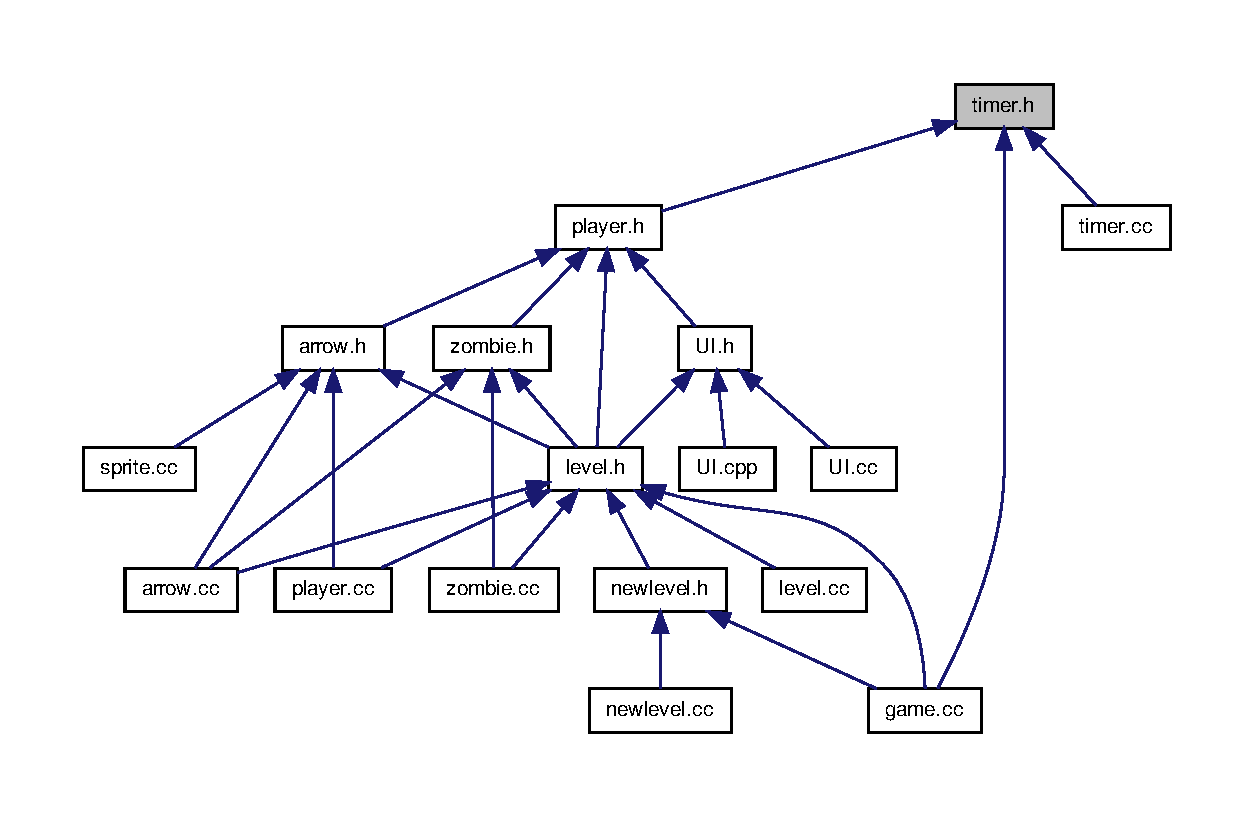
\includegraphics[width=350pt]{timer_8h__dep__incl}
\end{center}
\end{figure}
\subsection*{Classes}
\begin{DoxyCompactItemize}
\item 
class \hyperlink{classTimer}{Timer}
\end{DoxyCompactItemize}

\hypertarget{UI_8cc}{\section{U\-I.\-cc File Reference}
\label{UI_8cc}\index{U\-I.\-cc@{U\-I.\-cc}}
}
{\ttfamily \#include \char`\"{}U\-I.\-h\char`\"{}}\\*
Include dependency graph for U\-I.\-cc\-:\nopagebreak
\begin{figure}[H]
\begin{center}
\leavevmode
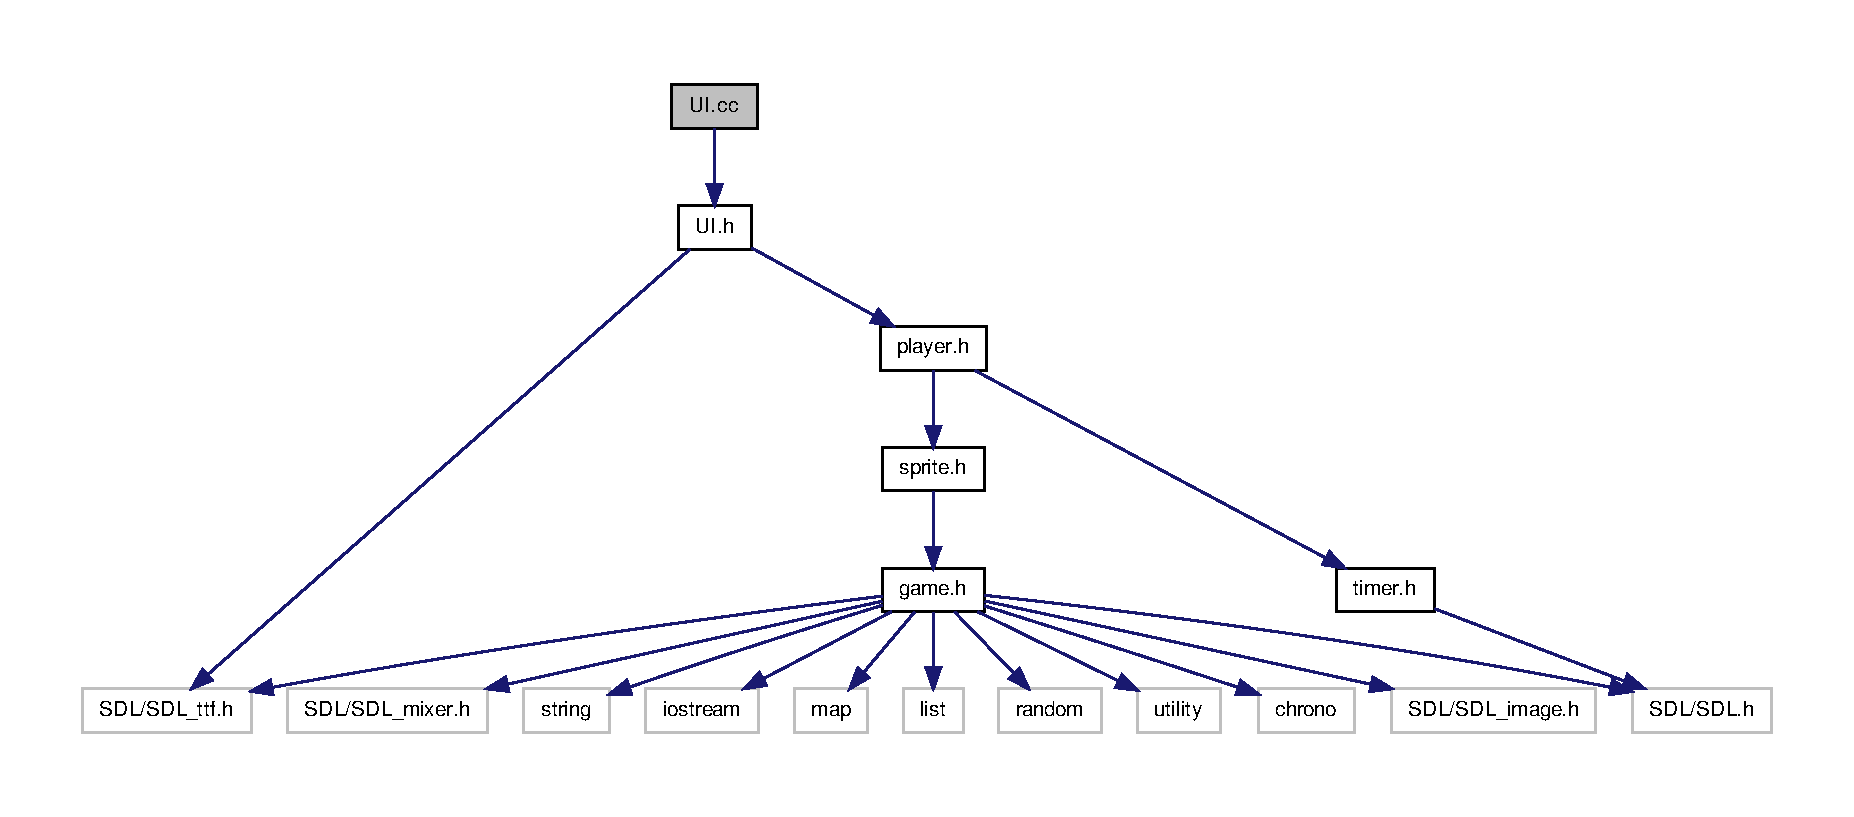
\includegraphics[width=350pt]{UI_8cc__incl}
\end{center}
\end{figure}

\hypertarget{UI_8cpp}{\section{U\-I.\-cpp File Reference}
\label{UI_8cpp}\index{U\-I.\-cpp@{U\-I.\-cpp}}
}
{\ttfamily \#include \char`\"{}U\-I.\-h\char`\"{}}\\*
Include dependency graph for U\-I.\-cpp\-:\nopagebreak
\begin{figure}[H]
\begin{center}
\leavevmode
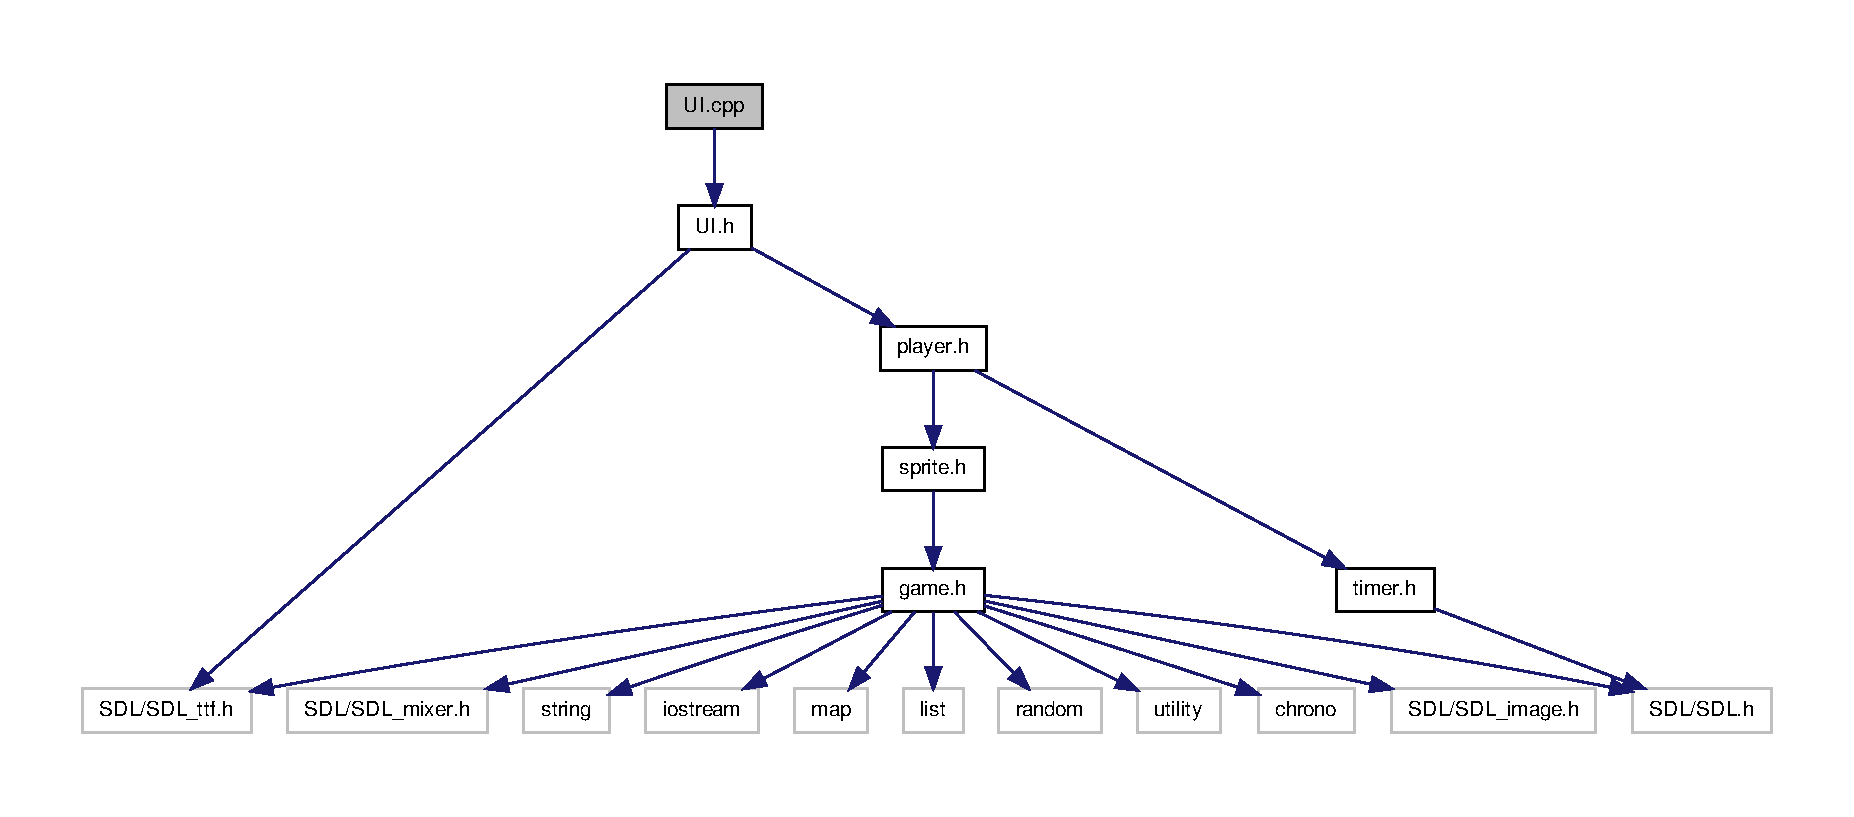
\includegraphics[width=350pt]{UI_8cpp__incl}
\end{center}
\end{figure}

\hypertarget{UI_8h}{\section{U\-I.\-h File Reference}
\label{UI_8h}\index{U\-I.\-h@{U\-I.\-h}}
}
{\ttfamily \#include $<$S\-D\-L/\-S\-D\-L\-\_\-ttf.\-h$>$}\\*
{\ttfamily \#include \char`\"{}player.\-h\char`\"{}}\\*
Include dependency graph for U\-I.\-h\-:\nopagebreak
\begin{figure}[H]
\begin{center}
\leavevmode
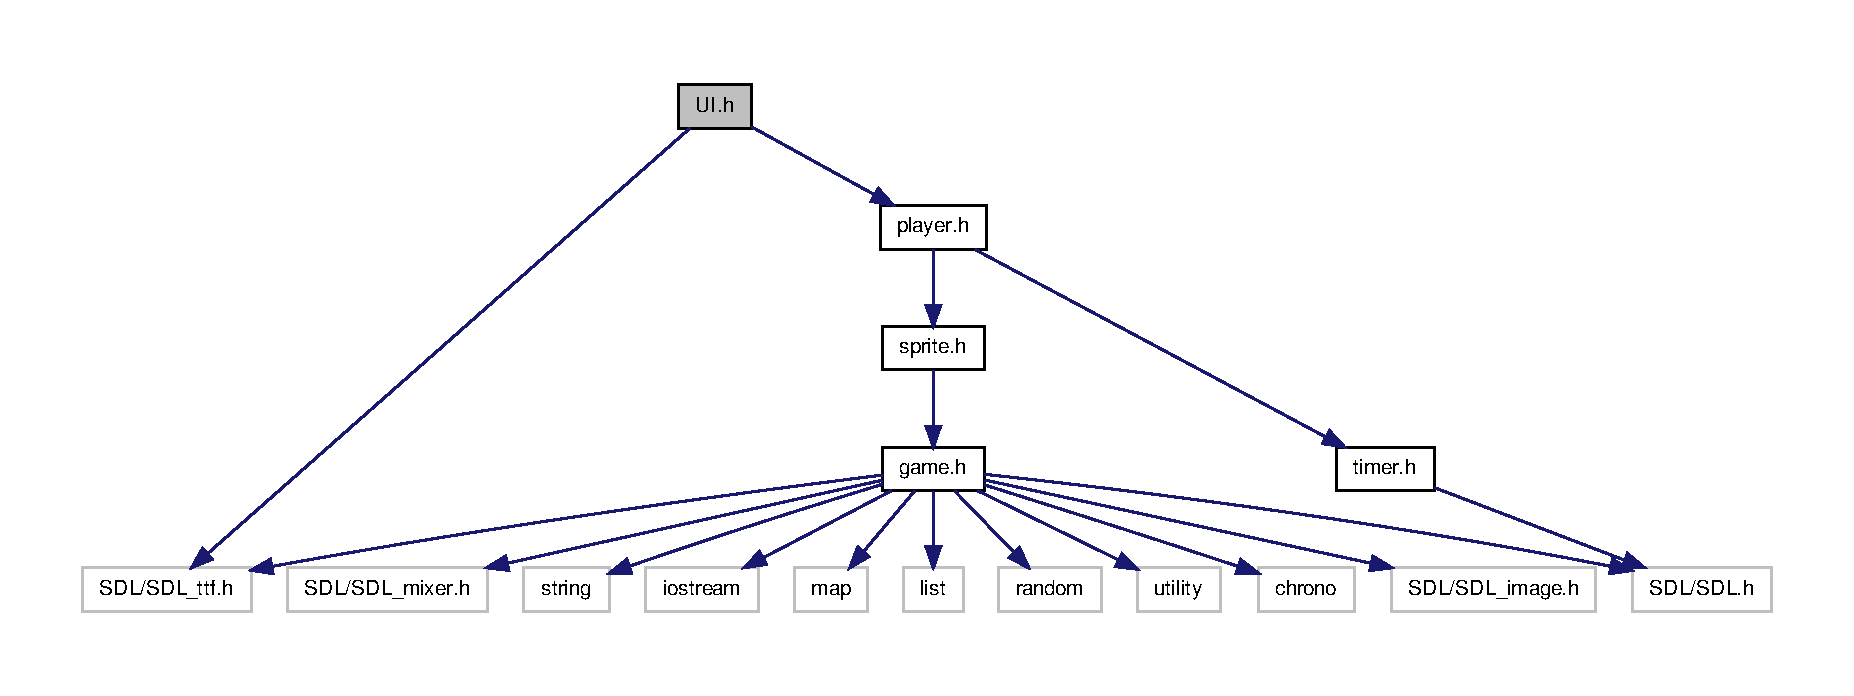
\includegraphics[width=350pt]{UI_8h__incl}
\end{center}
\end{figure}
This graph shows which files directly or indirectly include this file\-:\nopagebreak
\begin{figure}[H]
\begin{center}
\leavevmode
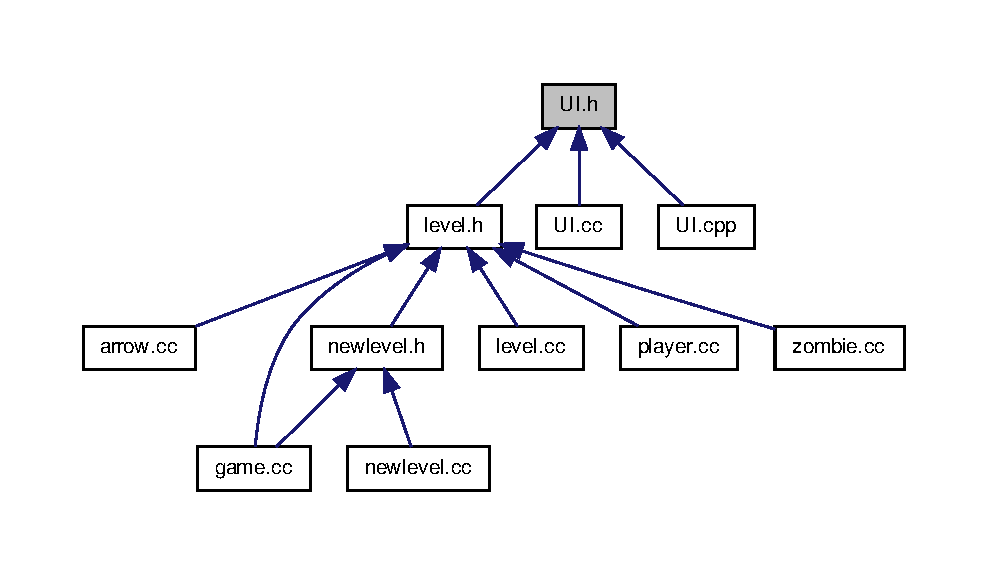
\includegraphics[width=350pt]{UI_8h__dep__incl}
\end{center}
\end{figure}
\subsection*{Classes}
\begin{DoxyCompactItemize}
\item 
class \hyperlink{classUi}{Ui}
\end{DoxyCompactItemize}
\subsection*{Macros}
\begin{DoxyCompactItemize}
\item 
\#define \hyperlink{UI_8h_a87b537f5fa5c109d3c05c13d6b18f382}{W\-H\-I\-T\-E}~\{255,255,255\}
\end{DoxyCompactItemize}


\subsection{Macro Definition Documentation}
\hypertarget{UI_8h_a87b537f5fa5c109d3c05c13d6b18f382}{\index{U\-I.\-h@{U\-I.\-h}!W\-H\-I\-T\-E@{W\-H\-I\-T\-E}}
\index{W\-H\-I\-T\-E@{W\-H\-I\-T\-E}!UI.h@{U\-I.\-h}}
\subsubsection[{W\-H\-I\-T\-E}]{\setlength{\rightskip}{0pt plus 5cm}\#define W\-H\-I\-T\-E~\{255,255,255\}}}\label{UI_8h_a87b537f5fa5c109d3c05c13d6b18f382}

\hypertarget{zombie_8cc}{\section{zombie.\-cc File Reference}
\label{zombie_8cc}\index{zombie.\-cc@{zombie.\-cc}}
}
{\ttfamily \#include \char`\"{}zombie.\-h\char`\"{}}\\*
{\ttfamily \#include \char`\"{}level.\-h\char`\"{}}\\*
Include dependency graph for zombie.\-cc\-:\nopagebreak
\begin{figure}[H]
\begin{center}
\leavevmode
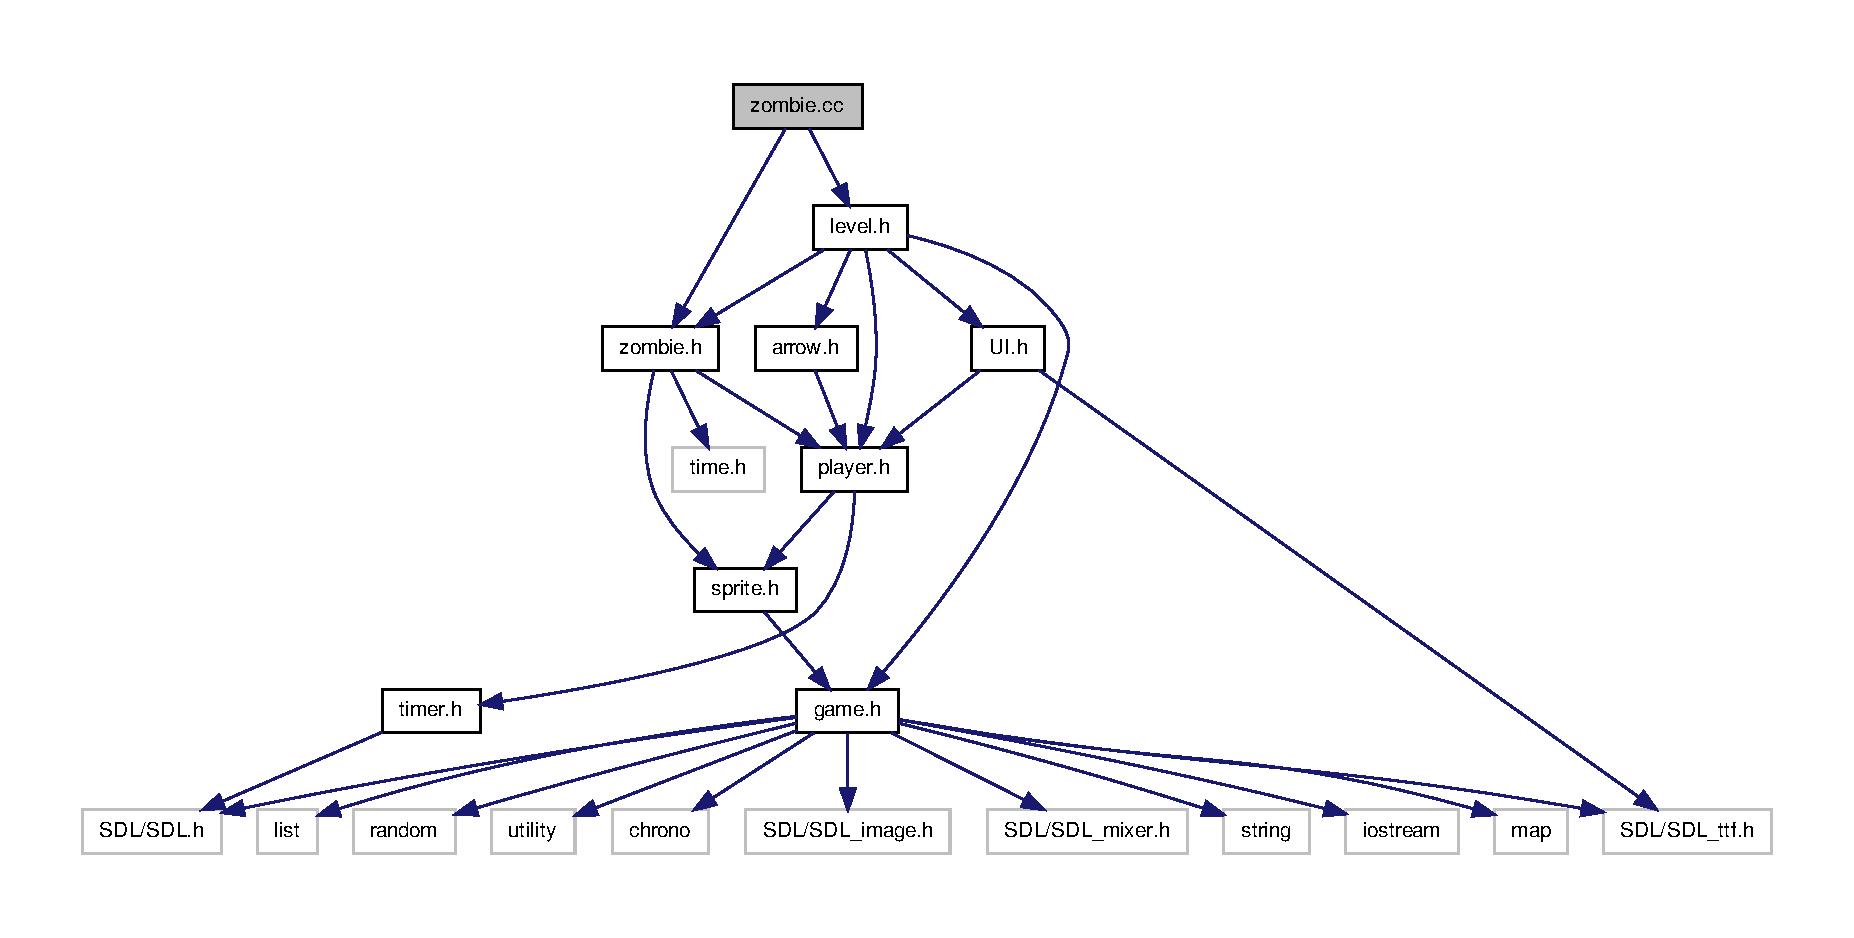
\includegraphics[width=350pt]{zombie_8cc__incl}
\end{center}
\end{figure}

\hypertarget{zombie_8h}{\section{zombie.\-h File Reference}
\label{zombie_8h}\index{zombie.\-h@{zombie.\-h}}
}
{\ttfamily \#include \char`\"{}sprite.\-h\char`\"{}}\\*
{\ttfamily \#include \char`\"{}player.\-h\char`\"{}}\\*
{\ttfamily \#include $<$time.\-h$>$}\\*
Include dependency graph for zombie.\-h\-:\nopagebreak
\begin{figure}[H]
\begin{center}
\leavevmode
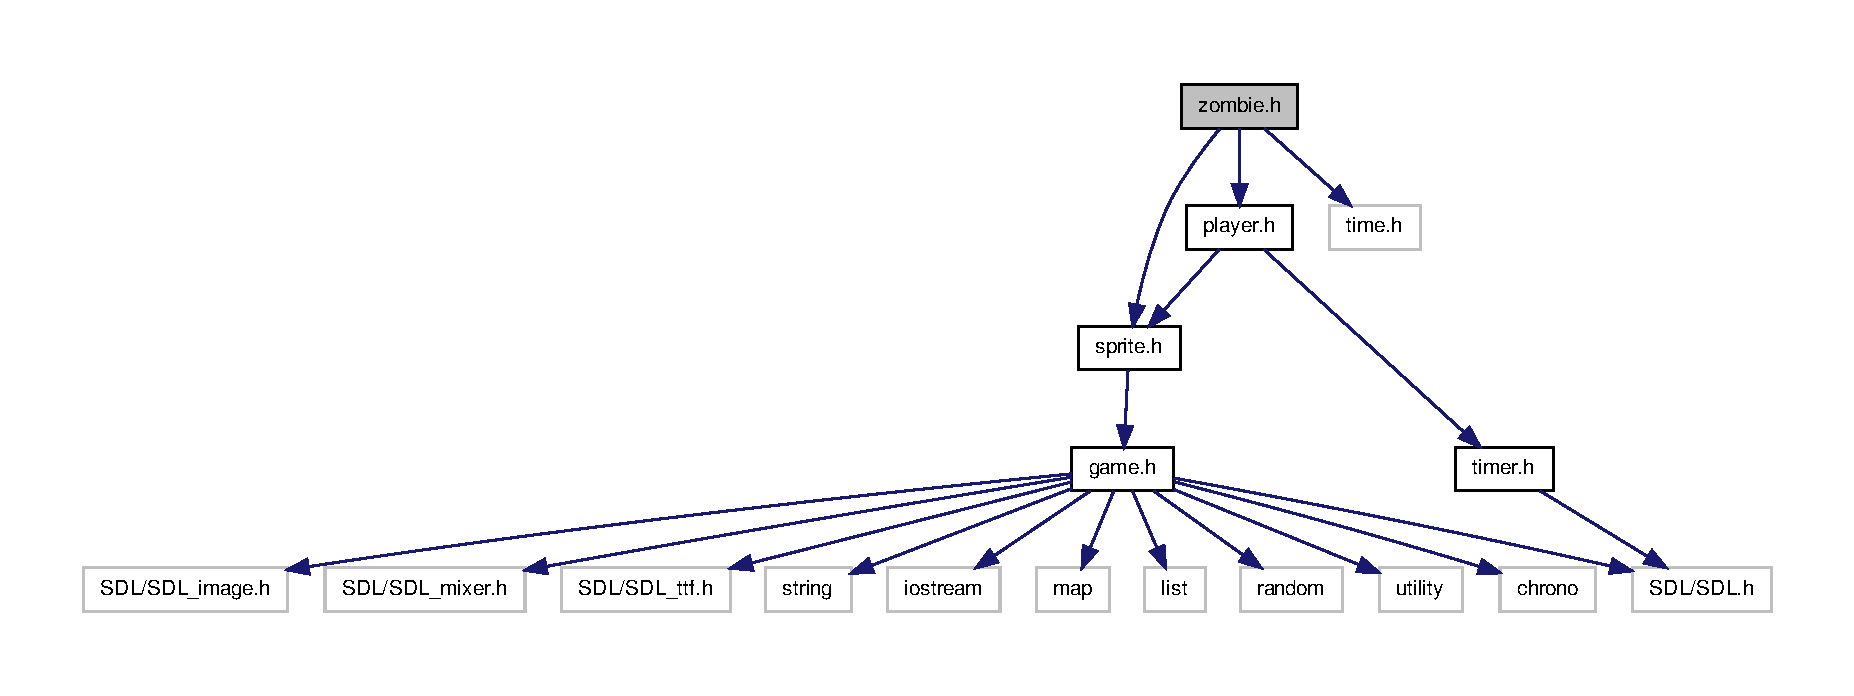
\includegraphics[width=350pt]{zombie_8h__incl}
\end{center}
\end{figure}
This graph shows which files directly or indirectly include this file\-:\nopagebreak
\begin{figure}[H]
\begin{center}
\leavevmode
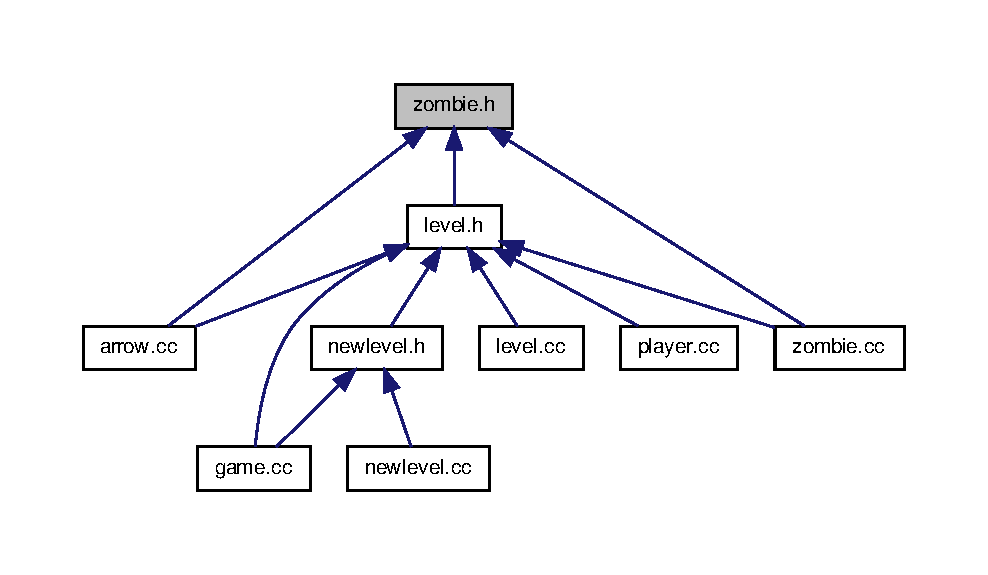
\includegraphics[width=350pt]{zombie_8h__dep__incl}
\end{center}
\end{figure}
\subsection*{Classes}
\begin{DoxyCompactItemize}
\item 
class \hyperlink{classZombie}{Zombie}
\end{DoxyCompactItemize}
\subsection*{Typedefs}
\begin{DoxyCompactItemize}
\item 
using \hyperlink{zombie_8h_a5d0af493672013a634b074e23582c518}{random\-Spawn\-Positions} = std\-::map$<$ std\-::string, std\-::pair$<$ int, int $>$ $>$
\end{DoxyCompactItemize}


\subsection{Typedef Documentation}
\hypertarget{zombie_8h_a5d0af493672013a634b074e23582c518}{\index{zombie.\-h@{zombie.\-h}!random\-Spawn\-Positions@{random\-Spawn\-Positions}}
\index{random\-Spawn\-Positions@{random\-Spawn\-Positions}!zombie.h@{zombie.\-h}}
\subsubsection[{random\-Spawn\-Positions}]{\setlength{\rightskip}{0pt plus 5cm}using {\bf random\-Spawn\-Positions} =  std\-::map$<$std\-::string, std\-::pair$<$int, int$>$ $>$}}\label{zombie_8h_a5d0af493672013a634b074e23582c518}

%--- End generated contents ---

% Index
\newpage
\phantomsection
\addcontentsline{toc}{chapter}{Index}
\printindex

\end{document}
